% !BIB program = biber
% !TeX root = main.tex

\documentclass[a4paper,12pt]{report}

\usepackage[english]{babel}
\usepackage[T1]{fontenc}
\usepackage[utf8]{inputenc}
\usepackage{newtxtext,newtxmath}
\usepackage{amsmath,amsfonts}
\usepackage{graphicx}
\usepackage{booktabs}
\usepackage{array}
\usepackage{tabularx}
\usepackage{caption}
\usepackage{subcaption}
\usepackage{float}
\usepackage{setspace}
\usepackage{csquotes}
\usepackage{vmargin}
\usepackage{titlesec}
\usepackage{listings}
\usepackage{xcolor}
\usepackage{algorithm}
\usepackage{algpseudocode}
\usepackage{mathtools}
\usepackage{tikz}
\usepackage{xurl}
\usepackage{hyperref}
\usepackage[style=ieee,sorting=none,backend=biber,defernumbers=true]{biblatex}
\addbibresource{bibliography.bib}
\setcounter{biburllcpenalty}{7000}
\setcounter{biburlucpenalty}{8000}
\setcounter{biburlnumpenalty}{9000}

\setmarginsrb{35mm}{30mm}{30mm}{30mm}{0mm}{10mm}{0mm}{10mm}
\hypersetup{
  colorlinks=true,
  linkcolor=black,
  citecolor=black,
  urlcolor=black,
  linktoc=all,
  bookmarksopen=true,
  plainpages=false
}

\setlength{\parindent}{1cm}
\setlength{\parskip}{0pt}
\onehalfspacing
\setlength{\emergencystretch}{2em}
\hfuzz=10pt
\hbadness=10000

\titleformat{\chapter}[display]
  {\bfseries\fontsize{16pt}{18pt}\selectfont}
  {\chaptertitlename\ \thechapter}
  {1ex}
  {}
\titleformat{\section}
  {\bfseries\fontsize{14pt}{16pt}\selectfont}
  {\thesection}
  {1em}
  {}
\titleformat{\subsection}
  {\bfseries\fontsize{12pt}{14pt}\selectfont}
  {\thesubsection}
  {1em}
  {}

\captionsetup{justification=centering}
\captionsetup[table]{position=top,font=small,labelfont=bf,justification=centering,singlelinecheck=false,skip=6pt}
\AtBeginEnvironment{figure}{\centering\captionsetup{position=bottom}}
\AtBeginEnvironment{table}{\centering\small}
\AtBeginEnvironment{algorithm}{\captionsetup{position=top,font=small,labelfont=bf,textfont=it}}
\floatname{algorithm}{Algorithm}
\floatstyle{ruled}
\restylefloat{algorithm}
\setlength{\textfloatsep}{16pt plus 2pt minus 2pt}
\setlength{\tabcolsep}{6pt}
\renewcommand{\arraystretch}{1.12}
\usetikzlibrary{arrows.meta,positioning,shapes.geometric,fit}

\lstdefinestyle{thesiscode}{
  basicstyle=\ttfamily\fontsize{10.5pt}{12pt}\selectfont,
  backgroundcolor=\color{gray!10},
  frame=single,
  rulecolor=\color{gray!40},
  xleftmargin=0pt,
  xrightmargin=0pt,
  showstringspaces=false,
  keepspaces=true,
  breaklines=true,
  tabsize=2,
  numbers=left,
  numberstyle=\tiny\color{gray!70},
  stepnumber=1,
  numbersep=8pt,
  captionpos=b
}
\lstset{style=thesiscode}

\definecolor{codebg}{RGB}{248,248,248}
\definecolor{codeframe}{RGB}{200,200,200}
\definecolor{codekw}{RGB}{0,112,32}
\definecolor{codecomment}{RGB}{96,96,96}
\definecolor{codestr}{RGB}{186,33,33}

\lstdefinestyle{pipeline}{
  language=Python,
  basicstyle=\ttfamily\footnotesize,
  keywordstyle=\color{codekw}\bfseries,
  commentstyle=\color{codecomment}\itshape,
  stringstyle=\color{codestr},
  backgroundcolor=\color{codebg},
  frame=single,
  rulecolor=\color{codeframe},
  breaklines=true,
  breakatwhitespace=false,
  showstringspaces=false,
  tabsize=4,
  xleftmargin=1.5em,
  framexleftmargin=1em,
  numbers=left,
  numberstyle=\tiny\color{gray},
  numbersep=8pt,
  captionpos=b,
  aboveskip=1em,
  belowskip=0.5em,
  morekeywords={as,with,None,True,False,self},
}

\algrenewcommand\algorithmicrequire{\textbf{Input:}}
\algrenewcommand\algorithmicensure{\textbf{Output:}}
\algrenewcommand\algorithmiccomment[1]{\hfill\footnotesize\upshape\color{black}(#1)}
\algrenewcommand\algorithmicindent{1.35em}
\algrenewcommand\algorithmicprocedure{\textbf{Procedure}}
\algrenewcommand\algorithmicend{\textbf{end}}
\algrenewcommand\alglinenumber[1]{\footnotesize\color{black!85}#1}
\AtBeginEnvironment{algorithmic}{\small}

\makeatletter
\renewcommand\footnotesize{\@setfontsize\footnotesize{10pt}{12pt}}
\makeatother

\begin{document}
\hypersetup{pageanchor=false}
\pagestyle{empty}

% Master thesis title page
{\thispagestyle{empty}

\vskip 1cm \large \centerline{\textsc{University of Naples Parthenope}}
\centerline{\textsc{Department of Science and Technologies}}
\centerline{\small\textsc{Master's Degree in Applied Computer Science in Machine Learning \& Big Data}}

\vskip 1.0cm
\begin{center}

\includegraphics[scale=0.20]{assets/logo_uniparthenope.png}
\end{center}

\vskip 0.5cm
\large \centerline{\textsc{Master's Thesis}}

\vskip 1.5cm
\Large \centerline{Feature-Driven Bias Detection}
\vskip 0.4cm
\large \centerline{An Association Rule Mining Approach to Analyze Feature Importance}

\vskip 2.0cm
\large
\begin{minipage}[t]{7cm}
\raggedright
\textsc{Supervisor}

\textbf{Prof. Antonio Maratea}
\vskip 0.6em
\textsc{Examiner}

\textbf{Prof. Francesco Camastra}
\end{minipage}
\hfill
\begin{minipage}[t]{5.8cm}
\textsc{Candidate}

\textbf{Alfredo Mungari}\\
\textbf{Student ID 0120000287}
\end{minipage}

\vskip 2em \Large \centerline{Academic Year 2024/2025}
\vskip 0.2em
\noindent\makebox[\textwidth][c]{\rule{0.55\textwidth}{0.5pt}}\par
\newpage}

\chapter*{Abstract}
\addcontentsline{toc}{chapter}{Abstract}
Modern tabular classifiers achieve strong predictive performance but remain opaque to inspection, particularly when their decisions involve demographic attributes. This thesis proposes a pipeline that combines counterfactual-based feature importance with hierarchical Association Rule Mining to produce a global, human-readable interpretation of a classifier's decision logic. The pipeline adapts the BoCSoR method from continuous to fully categorical data through a hybrid encoding and a Manhattan distance formulation, replacing continuous interpolation with the union of relevant feature-category pairs across $k$ observed opposite-class neighbors. The resulting local explanations are aggregated by a two-level mining procedure: a macroscopic level identifies structural dependencies at the feature-name level, and a microscopic level instantiates each surviving dependency with specific category values. A conservative semantic classification separates \emph{actionable} rules, involving only modifiable attributes, from \emph{biased} rules, involving protected demographic features. The pipeline is validated on five geographical benchmarks built from the 2024 American Community Survey (approximately 1.75 million records), using two structurally different classifiers (CatBoost and MLP) and a systematic grid search over support and confidence. The empirical study reveals a consistent geographic asymmetry: more affluent benchmarks (Northeast, New York) are dominated by actionable rules, while benchmarks with higher poverty concentration (Texas, South) are dominated by biased rules, with bias-to-actionable ratios ranging from $1.3\times$ to $11.8\times$. Race-occupation entanglement is the dominant biased signature in four of the five scopes, while the South uniquely exhibits a race-geography pattern. Rules at the higher-income boundary emerge only in New York. The main contributions are the adaptation of BoCSoR to categorical data, the hierarchical mining design, the semantic classification of rules, and the empirical characterization across U.S.\ census benchmarks.

\newpage
\tableofcontents
\listoffigures
\listoftables

\clearpage
\pagenumbering{arabic}
\setcounter{page}{1}
\pagestyle{plain}
\hypersetup{pageanchor=true}

\chapter{Introduction}
\label{cap:introduction}
% !TEX root = ../main.tex

\section{Context and Motivation}
\label{sec:intro-context}

Machine learning systems are increasingly deployed in consequential domains such as credit scoring, employment screening, healthcare triage, and public resource allocation. Their widespread use has exposed a growing tension between two intertwined requirements: on one side, the demand for predictive accuracy in large, heterogeneous datasets; on the other, the need for transparency and fairness in how decisions are made. Explainable Artificial Intelligence (XAI) has emerged as the research area tasked with addressing this tension, aiming to make the internal logic of black-box models intelligible to humans without compromising their predictive performance.

Within XAI, a distinction is often drawn between \emph{local} and \emph{global} explanation methods. Local explanations describe why a particular instance received a particular prediction, typically by perturbing features or examining nearby counterfactuals. Global explanations, by contrast, aim to characterize the overall behavior of the classifier, summarizing the recurring patterns that drive its predictions across the entire data distribution. Counterfactual-based methods have become a central tool in the local setting because they express importance in an operational form: a feature is relevant when modifying its value flips the prediction. However, aggregating many local counterfactual explanations into a coherent global picture remains an open problem, particularly in the presence of categorical attributes and protected demographic variables.

The present thesis addresses this problem by proposing a pipeline that combines counterfactual-based feature importance with Association Rule Mining (ARM) to extract a structured, global interpretation of a classifier's decision logic. The motivating application domain is income prediction on U.S.\ census data, where concerns about demographic bias intersect with the interpretability challenges of modern tabular classifiers. The goal is not to build a new predictor, nor to claim legal-grade evidence of discrimination, but to expose the patterns through which the classifier organizes its decisions and to distinguish, in a principled way, patterns that reflect modifiable attributes from patterns that rely on protected demographic features.

\section{Thesis Objectives}
\label{sec:intro-objectives}

The thesis pursues four objectives. The first is to adapt an existing boundary-based counterfactual method for feature importance, originally defined for continuous features, to the fully categorical setting obtained after preprocessing the ACS Income dataset. The second is to design a hierarchical Association Rule Mining procedure that operates on the local explanations produced by the adapted method, distinguishing structural dependencies (which features interact) from semantic content (which specific category values materialize those interactions). The third is to propose a semantic classification of the extracted rules that separates \emph{actionable} rules, involving only modifiable attributes, from \emph{biased} rules, involving protected demographic features. The fourth is to validate the pipeline empirically across multiple geographical benchmarks and classifier families, assessing whether the patterns it surfaces are consistent with the socio-economic structure of the underlying populations.

These objectives are motivated by the observation that macroscopic patterns alone do not provide sufficient explanatory depth (they indicate \emph{which} features matter but not \emph{how}), while microscopic patterns alone are too fragmented to yield a global picture. A hierarchical approach can combine the two levels, using macroscopic rules as a structural anchor for a more targeted microscopic analysis.

\section{Main Contributions}
\label{sec:intro-contributions}

The main contributions of this thesis are the following.

\begin{enumerate}
  \item \textbf{Adaptation of BoCSoR to categorical data.} The BoCSoR method, originally defined for continuous features, is adapted to the fully categorical setting obtained after preprocessing. The adaptation introduces a hybrid encoding (one-hot for nominal features, ordinal rank for ordered ones) and a Manhattan distance formulation that recovers the Hamming distance on the nominal component while preserving an ordered notion of similarity on the ordinal component. Interpolation, which is central in the original method but meaningless in a discrete space, is replaced by the use of $k$ observed opposite-class neighbors, aggregated through a union of per-neighbor relevant feature-category pairs.

  \item \textbf{Hierarchical macroscopic-to-microscopic Association Rule Mining.} A two-level ARM procedure is proposed. The macroscopic level operates on feature names only, identifying structural dependencies such as $\texttt{COW} \Rightarrow \texttt{OCCP}$. For each surviving macroscopic rule, the microscopic level examines the subset of transactions that instantiate it and mines value-level rules such as \texttt{COW=Local-Government-Employee} $\Rightarrow$ \texttt{OCCP=Educational-Instruction-And-Library}. The hierarchy reduces combinatorial explosion and provides a coarse-to-fine reading of the classifier's decision logic.

  \item \textbf{Semantic classification of rules (actionable, biased, other).} A conservative, mutually exclusive classification is introduced. Rules involving only features that an individual can in principle modify (education, class of worker, working hours, occupation) are labeled actionable; rules involving at least one protected demographic feature (sex, race) are labeled biased; all remaining rules are labeled other. This classification does not adjudicate the normative or legal status of the rules; it provides an operational lens for interpreting the pipeline's output.

  \item \textbf{Classifier-agnostic framework with systematic grid search.} The pipeline is validated using two structurally different classifiers, CatBoost and MLP, to separate model-specific artifacts from properties of the underlying data. To avoid dependence on a single pair of thresholds, the ARM stage performs a grid search over support and confidence, producing a full landscape of rule counts.

  \item \textbf{Large-scale empirical study on ACS 2024.} The pipeline is applied to five geographical benchmarks constructed from the 2024 American Community Survey via the Folktables framework: New York, Texas, the U.S.\ Northeast, the U.S.\ South, and the set of all U.S.\ states except Alaska (approximately 1.75 million records in total). The empirical study uncovers a systematic geographic asymmetry: more affluent and urbanized benchmarks (Northeast, New York) are dominated by actionable rules, whereas benchmarks with higher poverty concentration (Texas, South) are dominated by biased rules. The South additionally exhibits a unique bias pattern, $\texttt{RAC1P} \Rightarrow \texttt{POBP}$, that does not emerge as dominant elsewhere. Rules on the higher-income boundary are observed only in New York, and only for broad counterfactual neighborhoods.
\end{enumerate}

\section{Thesis Structure}
\label{sec:intro-structure}

The rest of the thesis is organized as follows. Chapter~\ref{cap:state-of-the-art} situates the contribution in the existing literature on counterfactual explanations, feature importance, Association Rule Mining, and fairness in tabular machine learning. Chapter~\ref{cap:data} describes the construction of the five benchmark datasets, the preprocessing pipeline, and the categorical schema adopted for all downstream analyses. Chapter~\ref{cap:method} formalizes the adapted BoCSoR procedure and the two-level hierarchical ARM, including the semantic classification of rules and the pseudocode of the three algorithms that constitute the pipeline. Chapter~\ref{cap:results} reports the experimental setup, the macroscopic results at three support thresholds, the decay analysis, the class asymmetry, the dominant macroscopic patterns, and the microscopic findings for each geographical scope. Chapter~\ref{cap:conclusions} summarizes the main findings, discusses the limitations of the approach, and outlines directions for future work. The appendices report implementation details, configuration and execution information, output artifacts, the software stack, and supplementary experimental data including classifier accuracy and dataset composition.

\chapter{State of the Art and Related Work}
\label{cap:state-of-the-art}
% !TEX root = ../main.tex

This chapter reviews the main strands of literature on which the thesis is grounded and shows how they converge within the proposed methodological framework. Rather than offering a generic overview of related work, it reconstructs the conceptual trajectory that motivates the thesis. The discussion begins with Explainable Artificial Intelligence (XAI), which provides the broader interpretive context in which this work is situated. It then turns to counterfactual explanations, which constitute the central explanatory perspective adopted in the thesis. From there, the chapter moves to feature selection and association-rule mining, two areas treated here not as isolated topics, but as essential components for the structured aggregation and analysis of counterfactual evidence.

This organization directly reflects the specific contribution of the thesis. The aim of the review is not merely to catalogue prior methods, but to show why the combination of local counterfactual evidence, feature-level relevance, and pattern-level synthesis helps address a gap that remains only partially covered in the existing literature. Accordingly, the chapter alternates between general survey material and explicit thesis positioning, so that each section contributes both to the state of the art and to the rationale underlying the proposed approach.

\section{Explainable Artificial Intelligence (XAI)}
Explainable Artificial Intelligence (XAI) is a field of research devoted to making machine-learning models and their predictions intelligible to human users. According to \textcite{adadi2018peeking}, \textcite{arrieta2020explainable}, and \textcite{molnar2022iml}, XAI seeks to clarify which factors influence a decision and how they contribute to the final output. The need for such methods has grown rapidly with the adoption of high-performing yet inherently opaque models, especially complex ensembles and deep neural networks, whose predictive accuracy is often achieved at the expense of interpretability. In the survey literature, \textcite{adadi2018peeking} and \textcite{arrieta2020explainable} describe this trade-off between predictive power and transparency as one of the central challenges of modern AI.

Within this context, XAI aims to make model behavior understandable and verifiable, enabling practitioners to validate learned patterns and detect potential failure modes. Explanations also support human decision-makers in high-stakes settings, where automated predictions must be interpreted critically rather than accepted passively. More broadly, explainability serves an important governance function by supporting accountability, trust, fairness assessment, and compliance-oriented reporting. As emphasized by \textcite{adadi2018peeking} and \textcite{arrieta2020explainable}, these needs arise across a wide range of application domains, although the concrete purpose of explanation varies with the decision context. In healthcare and biomedicine, explanations support clinical interpretation and make risk predictions more transparent. In finance and credit-risk analysis, they help justify automated assessments to analysts, auditors, and affected individuals. In industrial predictive-maintenance settings, they assist engineers in diagnosing failure patterns, distinguishing causal signals from noise, and prioritizing interventions. Similar demands arise in transportation and public-sector decision-support systems. For these reasons, XAI is now widely regarded as a foundational component of responsible AI pipelines rather than as a purely optional post-processing step.

\subsection{Bias, Fairness, and Their Connection with XAI}
The widespread deployment of machine-learning systems in socially relevant domains has made it clear that predictive performance alone is not sufficient to assess the quality of an AI system. Models often inherit and reproduce biases already present in historical data, data-collection procedures, labeling practices, or broader modeling choices. When these distortions disproportionately affect particular individuals or demographic groups, they raise serious fairness concerns. As discussed by Barocas and Selbst \cite{barocas2016big}, Mehrabi et al. \cite{mehrabi2021}, and, more broadly, Arrieta et al. \cite{arrieta2020explainable}, this issue is especially critical in domains such as credit scoring, hiring, insurance, healthcare, and public decision-support, where automated outputs can directly influence access to resources, opportunities, and rights.

In the machine-learning literature, \emph{bias} is a broad notion that refers to multiple sources of systematic distortion. A dataset may be biased because some populations are underrepresented, because labels reflect past discriminatory practices, or because some variables act as direct or indirect proxies for sensitive attributes. \emph{Fairness}, by contrast, concerns the extent to which a model and its decisions satisfy normative requirements of equitable treatment across individuals or groups. For this reason, fairness is typically studied through families of formal criteria, such as demographic parity, equal opportunity, equalized odds, calibration, and counterfactual fairness. As reviewed by Mehrabi et al. \cite{mehrabi2021}, discussed by Barocas and Selbst \cite{barocas2016big}, and extended in the counterfactual setting by Kusner et al. \cite{kusner2017counterfactual}, each criterion captures a different intuition of what a fair automated decision process should look like. Because these criteria are often mutually incompatible, fairness analysis is inherently contextual and requires explicit choices about which harms should be monitored and mitigated.

This close relationship is one of the main reasons fairness is so strongly connected to XAI. When a model produces systematically different outcomes across subpopulations, explanation methods are needed to determine whether such disparities arise from valid predictive structure, spurious correlations, or the undue influence of proxy variables. As emphasized by Arrieta et al. \cite{arrieta2020explainable} and Adadi and Berrada \cite{adadi2018peeking}, XAI methods support this diagnostic process by revealing which features drive predictions, highlighting whether local decisions depend on problematic variables, and helping assess whether the model relies on stable and plausible patterns rather than data artifacts. In this sense, explainability does not by itself guarantee fairness, but it does provide the analytical tools needed to inspect, contest, and document potentially unfair behavior.

The relationship is also bidirectional, because fairness requirements influence which explanations are considered useful in practice. In high-stakes settings, stakeholders want to know not only \emph{why} a prediction was made, but also whether similar individuals are treated consistently, whether sensitive information has implicitly influenced the output, and whether actionable changes can be suggested without reproducing discriminatory assumptions. From this perspective, XAI and fairness should be understood as complementary dimensions of responsible AI: fairness defines part of the evaluative objective, while XAI provides the interpretive mechanisms through which that objective can be examined and operationalized. This connection is particularly strong in the case of counterfactual explanations. Wachter et al. \cite{wachter2017counterfactual} show how such explanations reveal the role of modifiable attributes, Ustun et al. \cite{ustun2019actionable} highlight their relevance for actionable recourse, and Kusner et al. \cite{kusner2017counterfactual} connect them to asymmetric treatment patterns and fairness-sensitive forms of reasoning.

\subsection{XAI Methods: Classification and Taxonomy from Survey Literature}
Survey papers generally avoid forcing XAI methods into a single, mutually exclusive taxonomy. Instead, as shown by Guidotti et al. \cite{guidotti2018survey}, Adadi and Berrada \cite{adadi2018peeking}, and Arrieta et al. \cite{arrieta2020explainable}, they classify explanation methods along multiple complementary axes. In other words, XAI methods are not assigned to a rigid class, but are described through a combination of dimensions such as scope, access to the predictive model, and the form of the explanation.

A first major distinction separates \emph{intrinsic} from \emph{post-hoc} explainability. Intrinsic models, such as decision trees, sparse linear models, generalized additive models, and rule-based classifiers, are transparent by design and can therefore be inspected directly \cite{molnar2022iml,arrieta2020explainable}. Post-hoc methods, by contrast, are applied after training to explain the behavior of an otherwise opaque predictor. Representative examples include LIME \cite{ribeiro2016lime}, SHAP \cite{lundberg2017shap}, counterfactual explanations \cite{wachter2017counterfactual}, partial dependence plots \cite{friedman2001pdp}, and surrogate-rule extraction approaches \cite{guidotti2018survey,adadi2018peeking}.

A second major dimension concerns the scope of the explanation. Global explanations aim to reconstruct the model's overall behavior across a dataset. Classic examples include partial dependence analysis introduced by Friedman \cite{friedman2001pdp} and the broader global-explanation perspective reviewed by Arrieta et al. \cite{arrieta2020explainable}. Local explanations, by contrast, justify individual predictions and are especially useful when specific decisions must be defended. This local perspective is exemplified by LIME \cite{ribeiro2016lime}, SHAP \cite{lundberg2017shap}, counterfactual explanations \cite{wachter2017counterfactual}, and the wider taxonomy summarized by Guidotti et al. \cite{guidotti2018survey}.

Methods are also classified according to their relationship with the predictive model. \emph{Model-specific} approaches exploit architectural properties internal to the model, such as gradient-based saliency for neural networks or split-based importance measures for tree ensembles, a distinction emphasized by Arrieta et al. \cite{arrieta2020explainable}. \emph{Model-agnostic} approaches, instead, rely only on input--output behavior, which makes them applicable across heterogeneous predictive systems. Representative examples include LIME \cite{ribeiro2016lime}, SHAP \cite{lundberg2017shap}, and counterfactual explanations \cite{wachter2017counterfactual}; broader survey discussions by Guidotti et al. \cite{guidotti2018survey} and Adadi and Berrada \cite{adadi2018peeking} place these methods within the general model-agnostic family.

Finally, the literature distinguishes methods by the form of explanation they produce. Feature-attribution methods, such as SHAP \cite{lundberg2017shap} and saliency-based approaches discussed by Arrieta et al. \cite{arrieta2020explainable}, quantify the contribution of individual variables. Example-based methods instead use representative instances, including prototypes, that is, typical examples of a class; criticisms, that is, cases poorly represented by those prototypes; and counterfactuals, following the perspective of Wachter et al. \cite{wachter2017counterfactual} and Guidotti et al. \cite{guidotti2018survey}. Surrogate approaches approximate black-box behavior through simpler models, as in Ribeiro et al. \cite{ribeiro2016lime} and Molnar \cite{molnar2022iml}, whereas rule-based explanations express predictive logic through human-readable rules, a family discussed by both Guidotti et al. \cite{guidotti2018survey} and Arrieta et al. \cite{arrieta2020explainable}. Within this broad taxonomy, counterfactual explanation is the XAI method most central to this thesis because it provides the primary explanatory perspective through which feature relevance is analyzed.


\begin{table}[H]
\centering
\renewcommand{\arraystretch}{1.18}
\caption{Summary of the main taxonomy dimensions used to classify XAI methods.}
\label{tab:xai-taxonomy-summary}
\begin{tabular}{>{\raggedright\arraybackslash}p{0.22\textwidth} >{\raggedright\arraybackslash}p{0.24\textwidth} >{\raggedright\arraybackslash}p{0.39\textwidth}}
  \toprule
  \textbf{Dimension} & \textbf{Categories} & \textbf{Representative methods and models} \\
  \midrule
  Explainability design & Intrinsic; post-hoc & Decision trees, sparse linear models,\newline generalized additive models;\newline LIME, SHAP, counterfactual explanations,\newline partial dependence plots \\
  Explanation scope & Global; local & Global surrogate models,\newline partial dependence analysis,\newline aggregated feature-importance measures;\newline LIME, SHAP, counterfactual explanations \\
  Relation to predictive model & Model-specific; model-agnostic & Saliency-based methods for neural networks,\newline gain- or split-based importance measures for tree ensembles;\newline LIME, SHAP, permutation-based explanations,\newline counterfactual explanations \\
  Explanation form & Feature-attribution; example-based; surrogate; rule-based & SHAP and saliency-based methods;\newline prototypes, criticisms, and counterfactuals;\newline local linear surrogates and global interpretable proxies;\newline rule-extraction methods \\
  \bottomrule
\end{tabular}
\renewcommand{\arraystretch}{1.0}
\end{table}

\section{Counterfactual Explanations}
Counterfactual explanations answer explicit \enquote{what-if} questions by identifying the minimal changes to an input required to alter a model's prediction toward a desired outcome \cite{wachter2017counterfactual}. Intuitively, they describe how an instance must cross a decision boundary. In a lending scenario, for example, a counterfactual explanation can clarify why an application was rejected and which realistic changes could lead to approval. As highlighted by Chou et al. \cite{chou2022counterfactuals}, this contrastive structure is especially effective because it addresses the question of why one outcome occurred \emph{instead of} another plausible alternative. Their practical appeal lies in the fact that they express explanations within the same feature space as the original decision, thereby translating abstract model behavior into concrete feature-level variations.

Viewed through the taxonomy outlined above, the position of counterfactuals is relatively clear. Guidotti et al. \cite{guidotti2018survey} and Arrieta et al. \cite{arrieta2020explainable} generally classify them as post-hoc and local methods, while Wachter et al. \cite{wachter2017counterfactual} and Chou et al. \cite{chou2022counterfactuals} emphasize their model-agnostic and contrastive character. They are also typically interpreted as example-based explanations because they justify a decision by presenting a nearby alternative instance associated with a different outcome. This positioning is especially important for the present thesis: counterfactuals are not used here as global surrogates or as intrinsically interpretable models, but as local explanatory objects from which systematic information about feature relevance can be extracted. They occupy a particularly useful position within the XAI landscape because they preserve decision-specific detail while still allowing structured aggregation across many cases.

To be informative and practically useful, counterfactual explanations are typically evaluated against a set of core quality criteria. A well-constructed counterfactual should satisfy \emph{proximity} to the original instance while maintaining \emph{sparsity}, so that as few features as possible are changed and the explanation remains understandable. Moreover, the suggested changes cannot be purely mathematical artifacts: \emph{plausibility} requires the counterfactual to remain consistent with the underlying data distribution, while \emph{actionability} requires modified features to correspond to realistic and implementable interventions. Finally, when multiple recourse paths exist, \emph{diversity} becomes important because it gives users alternative ways of achieving a favorable outcome. Here, \emph{recourse} refers to the set of feasible changes through which an individual may obtain a desired decision outcome. This requirement is emphasized, from different perspectives, by Russell \cite{russell2019efficient}, Mothilal et al. \cite{mothilal2020explaining}, Poyiadzi et al. \cite{poyiadzi2020face}, and Karimi et al. \cite{karimi2022survey}.

These design principles make counterfactuals valuable not only for communicating individual predictions, but also for diagnosing local decision boundaries and identifying non-actionable dependencies, that is, cases in which the model relies on variables that the subject cannot realistically change. Counterfactuals are also useful for comparing alternative recourse paths and testing the coherence of a predictor under small perturbations, as shown in the foundational formulation of Wachter et al. \cite{wachter2017counterfactual}, the actionable-recourse perspective of Ustun et al. \cite{ustun2019actionable}, and the diversity-oriented framework of Mothilal et al. \cite{mothilal2020explaining}.

In the context of fairness, counterfactual reasoning plays a particularly important role. As explored by Kusner et al. \cite{kusner2017counterfactual} through the notion of \emph{counterfactual fairness}, these methods test whether a prediction remains stable when a sensitive attribute is hypothetically changed while all other relevant factors are held fixed. They are therefore highly informative for fairness auditing, because they can expose asymmetric recourse burdens, reveal when some demographic groups must undergo substantially larger changes to obtain a favorable outcome, and highlight decision patterns shaped by socially correlated variables. This function emerges clearly in the work of Kusner et al. \cite{kusner2017counterfactual}, Ustun et al. \cite{ustun2019actionable}, and Karimi et al. \cite{karimi2022survey}. Although counterfactuals do not replace formal fairness criteria, they provide a particularly concrete mechanism for inspecting unfair behavior.

For this thesis, the most important aspect of counterfactual explanations is their relationship with feature importance. In general, \emph{feature importance} refers to the extent to which an input variable contributes to a model's prediction, while \emph{relevant features} are those variables that carry decision-useful information for the task under study. Depending on the explanatory framework, relevance may refer to statistical contribution, predictive utility, or a more causal and decision-oriented notion of influence on the output. In the perspective adopted here, counterfactual analysis gives these notions an operational interpretation: a feature is considered especially relevant when modifying it is repeatedly necessary to flip the prediction, and its importance increases when it recurs across many valid and minimal counterfactuals. This yields a notion of \emph{decision-relevant feature importance} that is based not on variance decomposition alone, but on necessity for altering the prediction. In particular, Alfeo et al. \cite{alfeo2023bocsor} show that although counterfactuals are inherently local, aggregating them can yield stable global relevance signals. Closely related work by Mothilal et al. \cite{mothilal2021explaining} and Chou et al. \cite{chou2022counterfactuals} further shows that counterfactual explanations and feature-attribution methods should be viewed as complementary perspectives. This insight directly motivates the methodological approach of the thesis: local counterfactual structure is used as a bridge toward global, feature-level interpretation, and the resulting recurring patterns are subsequently summarized through association-based analysis.

\section{Feature Selection}
Feature selection aims to identify a subset of relevant variables that preserves or improves predictive utility while reducing redundancy and noise, as classically defined by Guyon and Elisseeff \cite{guyon2003introduction}. Beyond computational efficiency, it is also used to improve model interpretability, stability, and robustness. In the survey literature, Chandrashekar and Sahin \cite{chandrashekar2014survey} and Li et al. \cite{li2017feature} generally organize feature-selection methods into three broad families: \emph{filter} methods, which score features independently of the predictive model; \emph{wrapper} methods, which evaluate subsets through model performance; and \emph{embedded} methods, which integrate selection into the training process itself. Li et al. \cite{li2017feature} further extend this taxonomy to include distinctions such as supervised versus unsupervised selection, single-feature versus group selection, and optimization-based criteria.

Filter methods typically rely on mutual information, statistical tests, or correlation-based criteria. Wrapper methods search directly over subsets and often achieve strong predictive performance at a higher computational cost. Embedded methods include sparsity-inducing regularization and tree-based importance mechanisms, as discussed by Chandrashekar and Sahin \cite{chandrashekar2014survey} and by Li et al. \cite{li2017feature}. The same surveys also emphasize that no single family is uniformly superior; each embodies a different trade-off among predictive performance, computational cost, and interpretability.

Here, feature selection is approached through feature importance derived from counterfactual explanations. The underlying intuition is straightforward: if certain variables repeatedly appear in minimal counterfactual changes, they can be interpreted as especially relevant to crossing the decision boundary and revising the prediction. In this sense, counterfactual evidence does not merely accompany feature selection; it provides the explanatory basis on which variables are prioritized and constrained subsets are identified, especially when the objective is to emphasize actionable variables rather than simple predictive compression. This interpretation is consistent with the counterfactual relevance perspective developed by Alfeo et al. \cite{alfeo2023bocsor} and with the broader conceptual framing discussed by Chou et al. \cite{chou2022counterfactuals}. Recent work also investigates how instance-level counterfactual evidence can isolate features that are crucial for changing decisions in local neighborhoods, thereby complementing more classical feature-selection criteria, as discussed by Chen et al. \cite{chen2022causalfs} and Li et al. \cite{li2017feature}.

A related line of research explores association-rule-based feature selection. In this case, frequent rules identify variables that recur in discriminative combinations, so that importance emerges from interaction patterns rather than from marginal relevance alone. As noted by Hullermeier \cite{hullermeier2006association} and Ramírez-Gallego et al. \cite{ramirezgallego2014association}, rule-based methods are particularly useful when the goal is to preserve interpretability while still capturing multivariate structure. For the purposes of this thesis, this creates a natural complementarity: counterfactual explanations isolate the variables involved in a decision change, whereas association-oriented analysis summarizes how those variables interact across many explanations. Therefore, rather than proposing a new predictive feature-selection algorithm, this work uses counterfactual evidence to rank decision-relevant variables and to generate structured evidence that can support feature-selection reasoning.


\begin{table}[H]
\centering
\renewcommand{\arraystretch}{1.18}
\caption{Summary of the main taxonomy dimensions used to classify feature-selection methods.}
\label{tab:feature-selection-taxonomy-summary}
\begin{tabular}{>{\raggedright\arraybackslash}p{0.22\textwidth} >{\raggedright\arraybackslash}p{0.24\textwidth} >{\raggedright\arraybackslash}p{0.39\textwidth}}
  \toprule
  \textbf{Dimension} & \textbf{Categories} & \textbf{Representative criteria or methods} \\
  \midrule
  Selection family & Filter; wrapper; embedded & Mutual information, statistical tests; subset search with predictive models; L1 regularization, tree-based selection \\
  Learning setting & Supervised; unsupervised & Label-dependent relevance criteria; variance, similarity, or redundancy criteria \\
  Selection granularity & Single-feature; group-based & Ranking individual variables; selecting blocks or structured feature groups \\
  Optimization view & Ranking; subset search; regularized optimization & Score-based ordering; heuristic or exhaustive subset evaluation; sparsity-constrained training \\
  \bottomrule
\end{tabular}
\renewcommand{\arraystretch}{1.0}
\end{table}

\section{Association-Rule Mining: Taxonomy, Survey Perspective, and Relevance for This Thesis}
Association-rule mining (ARM) is a descriptive data-mining framework devoted to discovering recurring co-occurrence patterns. In its standard notation, a rule is written as $A \Rightarrow B$, where $A$ and $B$ are sets of items, usually called \emph{itemsets}. Intuitively, the rule states that when the items in $A$ appear together, the items in $B$ also tend to appear. In market-basket analysis, an item may literally be a purchased product; in more general analytical contexts, such as the one considered in this thesis, an item can instead represent a feature or a discretized feature-value condition. The classical foundations of ARM lie in the work of Agrawal and Srikant \cite{agrawal1994fast} and in the later pattern-growth perspective developed by Han et al. \cite{han2000mining}. Although originally introduced for market-basket analysis, ARM has since been applied to many other domains, including bioinformatics, fraud detection, and medical decision support, as discussed by Hullermeier \cite{hullermeier2006association} and Fournier-Viger et al. \cite{fournierviger2017survey}. Of particular relevance to this thesis is the work of Pedreschi, Ruggieri, and Turini \cite{pedreschi2008discriminationaware}, who proposed the use of association rules specifically for discrimination detection in automated decision systems. Their framework defines discriminatory classification rules as those whose confidence changes significantly when conditioned on a protected attribute, and it demonstrates that ARM can serve as a principled tool for identifying and quantifying bias in data-driven decisions. This line of research provides direct precedent for the interpretive use of association rules adopted in the present thesis, where extracted rules are examined for the presence of sensitive attributes as an indicator of potential bias in the classifier's decision logic. More broadly, the relevance of ARM lies in its ability to reveal structural interactions that often remain hidden in univariate analyses.

From a methodological standpoint, ARM proceeds in two main stages. First, it identifies recurrent feature combinations that satisfy a minimum \emph{support} threshold, that is, a minimum frequency of occurrence in the dataset. These combinations are usually called \emph{frequent itemsets}: an itemset is frequent when it appears in at least a user-defined proportion or count of transactions. Second, rules are derived from these frequent itemsets subject to additional interestingness constraints. In the rule $A \Rightarrow B$, $A$ is called the \emph{antecedent} and $B$ the \emph{consequent}. Among the most common evaluation measures are \emph{confidence}, which quantifies how reliably the consequent follows from the antecedent, and \emph{lift}, which compares the observed co-occurrence with what would be expected under statistical independence. These measures are central both in the classical presentations of Agrawal and Srikant \cite{agrawal1994fast} and Han et al. \cite{han2000mining}, and in later discussions of interestingness criteria such as that of McNicholas and Murphy \cite{mcnicholas2008lift}. As Hullermeier \cite{hullermeier2006association} emphasizes, they are essential for distinguishing trivial frequency from genuinely informative patterns.

The computation of frequent itemsets has historically been dominated by two major algorithmic paradigms. The first is candidate generation, exemplified by Apriori \cite{agrawal1994fast}, which builds larger itemsets level by level from smaller frequent ones and prunes the search space through the anti-monotonicity of support. The second is pattern growth, exemplified by FP-Growth \cite{han2000mining}, which avoids generating large numbers of explicit candidates by compressing the database into a prefix tree and recursively extracting frequent patterns from it. This distinction is especially important for the present thesis because the implementation adopted in the project relies specifically on FP-Growth. The choice is motivated by its practical efficiency when many recurring combinations must be explored and explicit candidate generation would become unnecessarily expensive.

Survey literature commonly organizes ARM along several complementary taxonomic dimensions. Hullermeier \cite{hullermeier2006association} and Fournier-Viger et al. \cite{fournierviger2017survey} both emphasize this multidimensional view. One dimension concerns the \emph{pattern type}, which ranges from classical frequent itemsets to sequential and high-utility patterns, moving from the foundational framework of Han et al. \cite{han2000mining} to the broader survey synthesis of Fournier-Viger et al. \cite{fournierviger2017survey}. A second dimension concerns the \emph{rule type}, which may be Boolean, quantitative, or fuzzy. Boolean rules express simple presence-or-absence conditions, quantitative rules involve numerical intervals or thresholds, and fuzzy rules allow gradual membership rather than sharp boundaries. This distinction is useful for positioning ARM within the broader literature; however, in the present thesis ARM is used only in its Boolean form, that is, by encoding whether an item is present or absent, and no fuzzy logic is adopted. A third dimension concerns the \emph{constraint setting}, including support thresholds, rule-length limits, and redundancy filters, all of which are essential because unconstrained mining often produces extremely large rule sets. A fourth dimension concerns the \emph{interestingness criterion}, which extends beyond support to include lift, leverage, and certainty factors. Finally, the \emph{algorithmic family} dimension contrasts candidate-generation methods such as Apriori \cite{agrawal1994fast} with pattern-growth approaches such as FP-Growth \cite{han2000mining}, directly reflecting the scalability issues discussed in the survey literature \cite{fournierviger2017survey}.

\begin{table}[H]
\centering
\renewcommand{\arraystretch}{1.18}
\caption{Summary of the main taxonomy dimensions used to classify association-rule mining methods.}
\label{tab:arm-taxonomy-summary}
\begin{tabular}{>{\raggedright\arraybackslash}p{0.22\textwidth} >{\raggedright\arraybackslash}p{0.24\textwidth} >{\raggedright\arraybackslash}p{0.39\textwidth}}
  \toprule
  \textbf{Dimension} & \textbf{Categories} & \textbf{Representative interpretation} \\
  \midrule
  Pattern type & Frequent; sequential; high-utility & Co-occurring itemsets; ordered patterns; quantity/value-aware patterns \\
  Rule type & Boolean; quantitative; fuzzy & Presence/absence rules; interval-based rules; gradual-membership rules \\
  Interestingness criteria & Support; confidence; lift & Frequency; conditional reliability; deviation from independence \\
  Algorithm family & Candidate generation; pattern growth & Apriori-style search; FP-Growth-style compressed mining \\
  Thesis setting & Boolean ARM; FP-Growth & Presence/absence encoding; efficient mining of frequent explanatory patterns \\
  \bottomrule
\end{tabular}
\renewcommand{\arraystretch}{1.0}
\end{table}

A crucial methodological issue concerns the treatment of multiplicities or quantities.
In classical ARM, each item is encoded in Boolean form: it is either present or absent in a transaction. This representation is not merely a simplifying assumption; it is the foundation that makes the anti-monotonicity of support operationally useful.
The anti-monotonicity property states that if an itemset is frequent, then all of its subsets must also be frequent; equivalently, if an itemset is infrequent, then all of its supersets must also be infrequent. This property allows classical frequent-itemset mining algorithms to efficiently prune large portions of the search space \cite{agrawal1994fast,han2000mining}.

When multiplicities are treated explicitly (e.g., distinguishing between one occurrence and multiple occurrences of the same item), this clean subset--superset ordering breaks, and the search space can no longer be reduced through the same anti-monotonic logic.
For this reason, multiplicities are not considered here: items are encoded strictly through presence or absence. This methodologically motivated choice allows the analysis to remain within the classical Boolean ARM framework, preserving the pruning structure required for efficient frequent-itemset mining, and aligns fully with the use of FP-Growth adopted in the implementation. In other words, neither fuzzy logic nor explicit item multiplicities are used in the thesis, precisely because the objective is to mine frequent explanatory patterns efficiently while preserving the anti-monotonic support structure on which the mining process depends.

Association rules offer several important advantages. They are inherently interpretable, because they can be read directly by domain experts without requiring access to a complex predictive model. They also capture multivariate interactions and support exploratory analysis and subgroup characterization, as highlighted by Hullermeier \cite{hullermeier2006association} and Fournier-Viger et al. \cite{fournierviger2017survey}. At the same time, the literature recognizes important limitations: ARM can generate very large and redundant rule sets, it is sensitive to preprocessing decisions, and naive reliance on confidence alone can be misleading. For this reason, modern ARM depends heavily on post-processing procedures and on multiple interestingness criteria, again in line with the discussions of Hullermeier \cite{hullermeier2006association} and McNicholas and Murphy \cite{mcnicholas2008lift}.

In the proposed pipeline, ARM is not treated as a standalone predictive technique, but as the mechanism through which explanation-derived evidence is synthesized at a global level. Counterfactual analysis provides local evidence about which features must change in order to alter the prediction; ARM then summarizes how these relevant features systematically co-occur across many explanations. In this setting, the extracted rules describe recurring structures in the explanations themselves rather than simple co-occurrence patterns in the raw data. More specifically, the approach leverages Boolean ARM with FP-Growth to efficiently extract frequent explanatory patterns while preserving the anti-monotonic support structure required by classical frequent-itemset mining. This role aligns closely with the objective of the thesis: to exploit the interpretability, multivariate expressive power, and filtering mechanisms of ARM in order to transform local counterfactual instances into a compact and human-readable global description of feature interactions and potential bias regularities.

\section{Literature Gap and Positioning of This Thesis}
The literature reviewed in this chapter provides a solid foundation for each component of the thesis, but it only partially addresses their integration within a unified explanatory pipeline. XAI research offers mature conceptual taxonomies and well-established interpretive objectives; counterfactual-explanation research provides effective local tools for analyzing decision changes; feature-selection literature clarifies how relevance can be formalized; and ARM literature offers efficient mechanisms for extracting recurrent patterns from structured data. What remains less explicitly developed is a framework that starts from local explanations, derives classifier-independent feature relevance from them, and then organizes that relevance into interpretable global patterns.

More specifically, the literature only partially covers the joint connection among:
\begin{itemize}
  \item local counterfactual explanations,
  \item feature relevance assessed independently of the specific classifier and inferred from decision-changing evidence,
  \item global pattern extraction through Boolean association-rule mining,
  \item and the subsequent analysis of rules that are actionable or potentially biased.
\end{itemize}

This is the precise point at which the thesis is positioned. The central idea is not merely to explain a classifier at the local level, but to use counterfactual explanations to identify which features most strongly influence the decision, independently of the particular predictive model adopted. In this sense, feature relevance is derived from the variables that repeatedly emerge in counterfactual changes, and these relevant features become the items used to build the ARM transactions. On top of this representation, the thesis applies Boolean ARM with FP-Growth and evaluates the extracted rules through support, confidence, and lift in order to identify stable global patterns, feature correlations, and explanatory regularities that would remain difficult to observe from isolated local explanations alone.

A second element that characterizes the thesis is the interpretive use of the extracted rules. The objective is not merely to mine frequent associations, but to examine which rules are actionable and which may reveal biased or otherwise problematic regularities. In this way, the framework connects local explanation, global feature relevance, rule-based pattern extraction, and bias-sensitive interpretation within a single methodological chain.

Finally, the thesis is also motivated by the practical difficulties associated with real-world datasets, including outdated information, incompleteness, inconsistent usage, and insufficient normalization. These data-related issues are not discussed in detail in this chapter because they are addressed in the following one, but they are already relevant for understanding the methodological choices made here. The need for robust local explanations, structured feature relevance, and interpretable rule extraction emerges precisely in settings where data quality cannot be taken for granted.

Overall, the state of the art supports the core methodological choice of the thesis: starting from local counterfactual explanations, deriving classifier-independent feature relevance, transforming those relevant features into Boolean ARM transactions, and using FP-Growth to extract frequent patterns that can then be interpreted through actionable and bias-related rules. The following chapters build directly on this rationale by describing the dataset and its criticalities, formalizing the method, and evaluating it empirically.

\chapter{Data and Dataset Construction}
\label{cap:data}
% !TEX root = ../main.tex

\section{Dataset Construction Overview}
This chapter describes how the reference dataset is constructed, including data sources, integration steps, and quality-control choices. The goal is to provide a transparent and reproducible description of the data pipeline used in this thesis.

\section{Limitations of Common Tabular Benchmarks}
\label{sec:benchmark-limitations}

This work focuses on the analysis of \emph{tabular} datasets, that is, datasets organized as rows of instances and columns of structured variables. In the fairness and explainability literature, empirical evaluation on tabular data has often relied on a relatively small set of reference benchmarks, most notably Adult and COMPAS, together with a few other recurring resources such as German Credit. Their popularity has made them useful as common points of comparison, but the literature increasingly stresses that they should not be treated as neutral or universally representative benchmarks.

A first issue concerns \emph{dataset size and empirical coverage}. By empirical coverage we mean the extent to which a dataset captures the diversity of cases, populations, and decision contexts that a method may encounter in practice. A benchmark has limited empirical coverage when it represents only a narrow slice of the relevant reality, for example because it is small, historically dated, geographically restricted, or based on a reduced set of variables. The methodological problem is that results obtained in such a setting can appear stronger and more stable than they actually are: a model may perform well only because the benchmark excludes many of the variations, edge cases, and structural heterogeneities present in real applications. In the specific case of Adult, the dataset is derived from a 1994 U.S. Census extract and contains fewer than fifty thousand instances, with only fourteen input features and a small set of protected attributes. As discussed by \textcite{ding2021retiring}, this historical and structural narrowness contributes to limited external validity, especially when modern fairness claims are generalized beyond the specific benchmark setting. The official UCI documentation also makes clear that Adult is a reasonably clean extract built from a much older census source and includes missing values in multiple categorical fields, which further highlights its constrained and partially incomplete nature \cite{kohavi1996adult}.

A second issue concerns \emph{anonymization, proxy structure, and limited semantic richness}. These concepts are related but distinct. By anonymization we mean the removal, aggregation, or masking of information that could identify individuals or institutions. Although this is necessary for privacy protection, it also removes context that may be crucial for understanding how the data were produced. By proxy structure we mean the presence of variables that, even if not explicitly sensitive themselves, may indirectly encode information about protected characteristics; for example, occupation, education, place of residence, or prior institutional contact may function as correlates of race, gender, or socioeconomic status. By limited semantic richness we mean that the variables and accompanying documentation are too sparse to reconstruct the substantive meaning of the observed attributes, labels, and exclusions. The practical consequence is that the analyst may not know what a variable truly measures, how a target label was generated, whether a feature acts as a hidden proxy for a sensitive attribute, or which social processes are missing from the dataset representation. As argued by \textcite{fabris2022story}, this is a broader problem in algorithmic-fairness datasets: anonymization, limited transparency, and weak documentation can obscure how sensitive attributes are encoded, how labels are produced, and what kinds of population exclusions or distortions are embedded in the data. In practice, this means that a benchmark may remain convenient for methodological comparison while still being poorly suited for substantive claims about fairness in realistic socio-technical settings.

A third issue concerns \emph{missing data, coding artifacts, and preprocessing errors}. While interconnected, these operational issues manifest differently in practice. Missing data are absent values in the table; the problem is not only the loss of information, but also the possibility that missingness is systematic and therefore introduces distortion. Coding artifacts are distortions produced by the way variables are encoded, discretized, cleaned, or exported, rather than by the underlying phenomenon itself. Preprocessing errors arise when undocumented transformations, merge decisions, label constructions, or cleaning steps alter the meaning of the data before analysis. These issues matter because downstream model performance and fairness assessments may then reflect properties of the benchmark construction rather than genuine methodological robustness. For Adult, missing categorical entries are part of the original resource \cite{kohavi1996adult}. For COMPAS, the critique is stronger: \textcite{bao2021compaslicated} argue that the benchmark abstraction hides substantial measurement bias and contextual complexity, making the dataset a poor fit for fairness benchmarking under assumptions of clean ground truth. More broadly, \textcite{fabris2022story} note that several widely used fairness benchmarks suffer from noisy data, severe coding mistakes, aging, and contrived prediction tasks, all of which call into question their role as general-purpose reference datasets.

These limitations do not imply that benchmark datasets such as Adult or COMPAS are useless. Rather, they indicate that results obtained on them must be interpreted cautiously and should not be overextended as evidence of robustness in realistic operational settings. This observation supports the motivation of the present thesis. Instead of relying only on small and highly reused benchmark datasets, the thesis is developed around a larger real-world tabular setting, where issues such as incompleteness, heterogeneity, semantic ordering, and data quality are treated as part of the methodological problem rather than abstracted away. In this sense, the choice of a large-scale census-based tabular dataset is not merely an application choice, but also a response to the limitations documented in the benchmark literature.

\section{From UCI Adult to Folktables: A Modern Census Alternative}
\label{sec:adult-to-folktables}
Since the empirical focus of this thesis is grounded in census data, it is necessary to examine the specific shortcomings of the UCI Adult dataset, which has long served as the \emph{de facto} standard for tabular machine learning and fairness evaluation. Derived from the 1994 Current Population Survey, Adult formulates a binary classification task asking whether an individual's income exceeds \$50,000. However, as comprehensively detailed by \textcite{ding2021retiring}, this specific formulation presents severe structural weaknesses for modern evaluation. First, the 1994 income threshold is highly outdated and no longer reflects meaningful socioeconomic boundaries without adjusting for inflation. Second, the dataset includes obscure coding artifacts, most notably the \texttt{fnlwgt} (final weight) feature. This variable was originally designed by the Census Bureau as a demographic multiplier to align the sample with aggregate population estimates, yet it is frequently and erroneously treated as a standard predictive feature in the machine learning literature. Finally, its fixed, single-year snapshot prevents any localized analysis, forcing researchers to evaluate fairness and explainability on a static and geographically monolithic population.

To overcome these criticalities, this thesis adopts the \emph{Folktables} framework introduced by \textcite{ding2021retiring} and available through the official Folktables repository \cite{folktablesrepo}. Folktables is not a single static dataset, but rather an open-source algorithmic interface that provides direct, reproducible access to the American Community Survey (ACS) Public Use Microdata Sample (PUMS) data made available by the US Census Bureau through its official ACS PUMS portal \cite{acspumsportal}. Instead of relying on a single, outdated historical threshold, Folktables allows researchers to synthesize datasets based on recent years and defines multiple standardized prediction tasks such as predicting employment status, medical coverage, or specific income percentiles. Furthermore, it supports state-level geographical stratification, meaning that data can be tailored to capture localized demographic distributions rather than relying on a generalized national average.

The transition from Adult to Folktables represents a methodological upgrade that closely aligns with the objectives of this work. By building the reference dataset through the Folktables API, the data-construction pipeline gains access to a significantly larger pool of instances, a more semantically rich set of contemporary features, and a transparent data-generation process. This transparent, large-scale environment is particularly well-suited for the proposed Association-Rule Mining (ARM) approach: the clarity, diversity, and reliability of the ACS features ensure that the extracted rules whether they capture global feature importance or potential algorithmic bias are grounded in meaningful socio-demographic realities rather than historical artifacts.

\section{The Folktables Framework}
\label{sec:folktables-framework}
The reference dataset used in this thesis is constructed through the \texttt{folktables} API, which operationalizes supervised-learning tasks from ACS PUMS microdata in a reproducible and standardized way \cite{ding2021retiring,folktablesrepo,acspumsportal}. These underlying ACS PUMS data are distributed by the US Census Bureau in an already anonymized public-use form, so that the \texttt{folktables} framework works on data that have already undergone disclosure-limitation procedures before entering the present pipeline. This does not eliminate the interpretive limitations associated with anonymization discussed in Section~\ref{sec:benchmark-limitations}, but it makes the provenance and institutional status of the anonymization process explicit from the outset. The main advantage of \texttt{folktables} is that it does not provide a single fixed table, but rather a configurable interface through which the researcher can choose the task, the filtering rule, the geographic scope, and the survey release used to instantiate the final analytical dataset.

The framework exposes multiple predefined ACS tasks that have become common reference points in the recent fairness literature. Each task corresponds to a distinct prediction problem built from ACS variables and labels. In the specific case of \texttt{ACSIncome}, the task is formulated as a binary classification problem in which the target indicates whether individual personal income lies below or above a given threshold. Table~\ref{tab:folktables-topics} summarizes the main topics provided by the framework together with their corresponding prediction targets.

\begin{table}[htbp]
\centering
\small
\renewcommand{\arraystretch}{1.15}
\caption{Summary of the main \texttt{folktables} topics and their associated prediction tasks.}
\label{tab:folktables-topics}
\begin{tabular}{>{\raggedright\arraybackslash}p{0.30\textwidth} p{0.26\textwidth} p{0.30\textwidth}}
  \toprule
  \textbf{Topic} & \textbf{Prediction target} & \textbf{Task meaning} \\
  \midrule
  \texttt{ACSIncome} & Personal income threshold & Predict whether annual personal income exceeds a specified threshold. \\
  \texttt{ACSPublicCoverage} & Public health coverage & Predict whether a person is covered by public insurance. \\
  \texttt{ACSMobility} & Residential mobility & Predict whether a person changed residence within the last year. \\
  \texttt{ACSEmployment} & Employment status & Predict whether a person is employed. \\
  \texttt{ACSTravelTime} & Commute-time threshold & Predict whether travel time to work exceeds a threshold. \\
  \bottomrule
\end{tabular}
\renewcommand{\arraystretch}{1.0}
\end{table}

In addition to task choice, \texttt{folktables} also makes explicit the sample restrictions associated with each problem formulation. This is an important advantage over many benchmark datasets, because it clarifies which observations are retained, which are excluded, and under which assumptions the learning problem is defined. Table~\ref{tab:folktables-filters} summarizes the main filters associated with the best-known \texttt{folktables} topics.

\begin{table}[htbp]
\centering
\renewcommand{\arraystretch}{1.2}
\caption{Main \texttt{folktables} topics and associated preprocessing filters.}
\label{tab:folktables-filters}
\begin{tabular}{>{\raggedright\arraybackslash}p{0.30\textwidth} p{0.60\textwidth}}
  \toprule
  \textbf{Topic} & \textbf{Filter conditions} \\
  \midrule
  \texttt{ACSIncome} (\texttt{adult\_filter}) & Individuals older than 16, with positive usual working hours and personal income above a minimum threshold. \\
  \texttt{ACSPublicCoverage} & Individuals selected according to the public-coverage task definition implemented by \texttt{folktables}. \\
  \texttt{ACSMobility} & Individuals retained according to the mobility-task filter defined in the framework. \\
  \texttt{ACSEmployment} & Working-age individuals retained by the employment-task filter. \\
  \texttt{ACSTravelTime} & Employed individuals retained by the travel-time task filter. \\
  \bottomrule
\end{tabular}
\renewcommand{\arraystretch}{1.0}
\end{table}

Taken together, these options make \texttt{folktables} more transparent and configurable than traditional fixed benchmarks. The researcher can specify not only the target problem, but also the population slice on which that problem is instantiated, thereby making the data-construction logic an explicit part of the documented methodology rather than an implicit preprocessing detail.

\section{Sources and Downloaded Data}
\label{sec:dataset-preparation}

Within this broader framework, the analytical dataset is instantiated by selecting the \texttt{ACSIncome} task. In \texttt{folktables}, \texttt{ACSIncome} is the task that formulates income prediction as a binary classification problem derived from ACS variables, where the target indicates whether an individual's personal income exceeds the threshold defined by the task specification. This choice preserves continuity with the income-prediction setting historically associated with Adult while replacing the older benchmark with a more recent and better documented census source. The dataset is generated by applying the standard \texttt{adult\_filter} used by \texttt{folktables}, which retains individuals older than 16 with positive weekly working hours and personal income above a minimum reporting threshold. In addition, records with null values are excluded from the analytical table, and duplicate observations are removed during raw-data acquisition and assembly. Using this predefined filter improves comparability with prior work while avoiding ad hoc sample restrictions at the data-construction stage.

The data-construction pipeline relies entirely on the 2024 ACS release. This year was selected because it is the most recent ACS release for which the required data are available in a sufficiently complete form for the present study. Starting from this common source, the pipeline generates five dataset instances corresponding to the five geographical benchmark groups considered in the thesis: the New York metropolitan area, Texas, the U.S. Northeast, the U.S. South, and the set of all U.S. states except Alaska. The two regional benchmarks follow the standard Census geography. More precisely, the Northeast comprises Maine, New Hampshire, Vermont, Massachusetts, Rhode Island, Connecticut, New Jersey, New York, and Pennsylvania, whereas the South comprises Delaware, Maryland, the District of Columbia, Virginia, West Virginia, North Carolina, South Carolina, Georgia, Florida, Kentucky, Tennessee, Alabama, Mississippi, Arkansas, Louisiana, Oklahoma, and Texas \cite{censusregions}.

For this analysis, the New York metropolitan area and Texas are treated as small-scale benchmarks, while the Northeast and the South are used as medium-scale benchmarks. This choice is motivated not only by dataset size, but also by the intention to compare the proposed pipeline across socio-economically contrasting settings. The New York benchmark is intended to capture a dense metropolitan context; this interpretation is coherent with the Census definition of a metropolitan statistical area as a territorially integrated area organized around a large urban core and its commuting ties \cite{censusmetroglossary}. Within this comparative design, New York is used as the more affluent and urbanized pole of the small-scale comparison, while Texas is used as the contrasting benchmark. This characterization is supported, at the state level, by Census indicators reporting higher median household income and lower poverty in New York than in Texas \cite{quickfactsny,quickfactstx}. The same logic guides the regional comparison: the Northeast is used as the more affluent benchmark, whereas the South is used as the contrasting benchmark. This choice is consistent with Census regional profile data for the Northeast and with recent Census evidence showing that sustained high-poverty counties are concentrated disproportionately in the South \cite{censusnortheastprofile,censussouthpoverty}.

Finally, the benchmark including all U.S. states except Alaska serves as the large-scale reference dataset. In the 2024 instantiation used in this thesis, the five benchmark datasets contain between 106,877 and 1,753,049 records after applying the \texttt{ACSIncome} task filter and then selecting the corresponding geographic benchmark. By contrast, the corresponding ACS 2024 extraction used in the project contains 2,956,351 records in total before benchmark-specific geographic selection. Table~\ref{tab:dataset-cardinality} summarizes the cardinality of each dataset.

\begin{table}[htbp]
\centering
\renewcommand{\arraystretch}{1.2}
\caption{Number of records in the five benchmark datasets and in the full ACS 2024 extraction.}
\label{tab:dataset-cardinality}
\begin{tabular}{>{\raggedright\arraybackslash}p{0.42\textwidth} p{0.24\textwidth}}
  \toprule
  \textbf{Dataset} & \textbf{Number of records} \\
  \midrule
  New York metropolitan area & 106,877 \\
  Texas & 145,670 \\
  U.S. Northeast & 308,138 \\
  U.S. South & 642,617 \\
  All U.S. states except Alaska & 1,753,049 \\
  Full ACS 2024 extraction & 2,956,351 \\
  \bottomrule
\end{tabular}
\renewcommand{\arraystretch}{1.0}
\end{table}

Taken together, these five datasets are used not only to assess the thesis pipeline under different input sizes, but also to compare its behavior across tabular settings that differ in distributional structure, sparsity, demographic composition, and overall socio-economic profile. 

\subsection{Synthetic Data Augmentation via Diffusion Models}
\label{sec:synthetic-augmentation}

The final datasets used in this thesis are not limited to the original ACS records selected through the pipeline described above. After the raw extraction and cleaning stage, and before the categorization steps applied to the analytical table, the data are augmented with synthetic samples in order to increase empirical variability and reduce the risk that the downstream analysis reflects only the specific realization of the observed census slice. This augmentation is performed on the pre-categorized table, that is, when the data still contain both numerical and categorical columns in their original mixed-type form. Consequently, the synthetic-generation stage takes place before the categorization of continuous variables discussed in Section~\ref{sec:discretization} and before the aggregation of the occupational code \texttt{OCCP} described in Section~\ref{sec:occp}.

To generate synthetic records, the pipeline adopts a diffusion-based tabular generator inspired by \textcite{shi2025tabdiff}. TabDiff is specifically designed for mixed-type tabular data and models numerical and categorical attributes jointly while preserving their distinct statistical nature. Its main methodological advantage, for the purposes of this thesis, is that the forward diffusion and reverse denoising dynamics are not imposed uniformly on the whole table. Instead, they are adapted feature-wise, so that each column can follow a diffusion process coherent with its own distributional properties. This is particularly useful in the present setting, where the raw ACS table combines continuous quantities such as age, hours worked, and income with categorical variables characterized by heterogeneous cardinalities and highly non-uniform empirical frequencies. According to the authors, TabDiff introduces a joint continuous-time diffusion framework for numerical and categorical data, with feature-wise learnable diffusion processes designed to account for the heterogeneity of different columns \cite{shi2025tabdiff}.

From an operational perspective, the synthetic generator is used as a data-augmentation component rather than as a replacement for the original sample. The objective is not to create an alternative benchmark disconnected from the observed ACS distribution, but to enrich the available training data with additional plausible records that preserve the structural dependencies among variables while increasing the diversity of the resulting dataset. For this reason, the augmentation is inserted at the raw-data level, before the handcrafted transformations that are specific to the analytical pipeline. This design ensures that the subsequent categorization, occupational aggregation, train--test split, and rule-mining stages are applied uniformly to both original and synthetic records.

The quality of the generated data is assessed by comparing the synthetic tables with the corresponding original tables along two complementary dimensions. First, the correlation structure of the variables is analyzed to verify that the synthetic data preserve the main inter-feature dependencies present in the original observations. More precisely, the comparison is based on both Pearson correlation and Spearman rank correlation, to evaluate preservation of linear dependence as well as monotonic dependence. Second, fairness-related metrics are computed on the original and generated data and then compared to evaluate whether the synthetic augmentation alters the sensitive structure of the benchmark. In particular, the fairness assessment considers False Positive Error Rate Balance, False Negative Error Rate Balance (equivalently discussed in relation to Equal Opportunity), Equalized Odds, and Overall Accuracy Equality. Preliminary evaluations confirmed that the synthetic data remain closely aligned with the original data: both the correlation patterns and the considered fairness indicators are similar, and in several cases effectively indistinguishable, between the two sources. This empirical similarity supports the use of the augmented datasets as a faithful extension of the original ACS-derived benchmarks rather than as a distributionally shifted surrogate.

\section{Dataset Composition and Feature Schema}
\label{sec:dataset-columns}

All five benchmark datasets share the same column structure defined by the \texttt{ACSIncome} task. Since \texttt{ACSIncome} is formulated as a binary classification problem, each resulting table comprises both a set of inputs and a target label. The attributes included across all datasets are \texttt{AGEP} (age), \texttt{COW} (class of worker), \texttt{SCHL} (educational attainment), \texttt{MAR} (marital status), \texttt{OCCP} (occupation code), \texttt{POBP} (place of birth), \texttt{RELP} (relationship to the household reference person), \texttt{WKHP} (weekly working hours), \texttt{SEX} (reported sex), and \texttt{RAC1P} (reported race). Alongside these predictors is a binary outcome derived from \texttt{PINCP} (individual income). The complete feature schema and variable characteristics are summarized in Table~\ref{tab:acsincome-feature-schema}.

These attributes, however, are not treated uniformly throughout the data pipeline. Depending on their source format and functional role, numerical variables may be categorized, while categorical ones require harmonization and profiling. Furthermore, some features preserve an ordinal interpretation, whereas others are explicitly designated as protected, contextual, or actionable during the experimental phase. 

The following sections provide a detailed description of each attribute's meaning, its role within the explanatory framework, and the specific data preparation operations applied, including categorization criteria and source definitions. These structural choices directly inform both the methodological approach described in Chapter~\ref{cap:method} and the experimental evaluations discussed in Chapter~\ref{cap:results}. Ultimately, these procedures ensure internal coherence while bolstering the reliability and interpretability of the downstream analysis.

Following the application of the standard task filter and the aforementioned processing steps, each of the five tabular datasets is partitioned into training and test subsets using an 80\%/20\% split. This configuration serves as the foundation for the subsequent predictive and explanatory evaluations.

\begin{table}[htbp]
\centering
\renewcommand{\arraystretch}{1.2}
\caption{Summary schema of the main variables in the selected \texttt{ACSIncome} task.}
\label{tab:acsincome-feature-schema}
\begin{tabular}{>{\raggedright\arraybackslash}p{0.16\textwidth} p{0.24\textwidth} p{0.50\textwidth}}
  \toprule
  \textbf{Column} & \textbf{Type} & \textbf{Summary description} \\
  \midrule
  \texttt{AGEP}  & Numerical (then discretized) & Individual age. \\
  \texttt{WKHP}  & Numerical (then discretized) & Weekly hours worked. \\
  \texttt{COW}   & Categorical & Class of worker (for example private, public, or self-employed). \\
  \texttt{SCHL}  & Ordinal categorical & Educational attainment. \\
  \texttt{MAR}   & Categorical & Marital status. \\
  \texttt{OCCP}  & Encoded categorical & Occupation code. \\
  \texttt{POBP}  & Encoded categorical & Place of birth. \\
  \texttt{RELP}  & Categorical & Relationship to household reference person. \\
  \texttt{SEX}   & Binary categorical & Reported sex in the ACS coding scheme. \\
  \texttt{RAC1P} & Categorical & Reported race in the ACS coding scheme. \\
  \bottomrule
\end{tabular}
\renewcommand{\arraystretch}{1.0}
\end{table}

\subsection{Income Binarization Threshold}
The target variable of our dataset is derived from \texttt{PINCP}, the ACS variable corresponding to individual personal income, through the binary task definition associated with \texttt{ACSIncome}. Within the \texttt{folktables} interface, \texttt{PINCP} is binarized into the values $0$ and $1$ on the basis of an income threshold, here denoted by $\theta$. In its standard configuration, $\theta$ is set at \$50,000, thereby preserving continuity with the classical UCI Adult formulation, although it can in principle be redefined by the user at dataset-construction time. Under this encoding, value $0$ corresponds to the lower-income class, whereas value $1$ identifies the medium-to-higher-income class.

For the reasons discussed in the previous sections, the standard \$50,000 threshold is not suitable for any of the five datasets considered in this thesis, since it does not adequately reflect either the geographic heterogeneity of the selected areas or the socioeconomic conditions of the reference year 2024. We therefore adopt a territory-specific threshold that remains coherent with the economic conditions of 2024 and can be applied directly to individual income.

More precisely, we follow the criterion adopted by the Pew Research Center to identify the point at which an individual enters the middle-to-upper-income class. According to this criterion, an individual belongs to the middle-to-upper-income class when income reaches at least twice the mean individual income of the territory under analysis, here denoted by $M_{\mathrm{ind}}$~\cite{pew2024middleclassmethodology,kochhar2022pew}. Operationally, in our datasets, $M_{\mathrm{ind}}$ is computed directly from the raw \texttt{PINCP} values extracted through \texttt{folktables}, since \texttt{PINCP} records the individual personal income associated with each observation. The threshold is therefore defined as
$$
  \theta \;=\; 2 \cdot M_{\mathrm{ind}},
$$
and is interpreted as the minimum individual income required for an observation to be assigned to the middle-to-upper-income class in the corresponding geographic context. Table~\ref{tab:income-thresholds} summarizes the resulting threshold values used for the five datasets considered in this thesis.

\begin{table}[htbp]
\centering
\renewcommand{\arraystretch}{1.2}
\caption{Income binarization thresholds adopted for the five datasets considered in this thesis.}
\label{tab:income-thresholds}
\begin{tabular}{>{\raggedright\arraybackslash}p{0.34\textwidth} p{0.26\textwidth}}
  \toprule
  \textbf{Dataset} & \textbf{Threshold $\theta$} \\
  \midrule
  \texttt{ALL} & \$94{,}200 \\
  \texttt{Northeast} & \$100{,}700 \\
  \texttt{South} & \$86{,}000 \\
  \texttt{NY} & \$94{,}400 \\
  \texttt{TX} & \$90{,}800 \\
  \bottomrule
\end{tabular}
\renewcommand{\arraystretch}{1.0}
\end{table}

\subsection{Categorization of Continuous Features}
\label{sec:discretization}
Among the variables extracted into our datasets, two features, \texttt{AGEP} (age) and \texttt{WKHP} (weekly hours worked), are numerical in their raw form. However, unlike purely nominal variables, both exhibit an intrinsic order relation among their values: for example, an age value of 20 denotes a lower age than a value of 50, and 20 weekly working hours denote a shorter schedule than 50 hours. To align these variables with the rest of the dataset and to represent them in a format directly manageable by the ARM pipeline, we transform them into ordinal categorical features through categorization. This choice is also consistent with the treatment of numerical variables formalized in the dedicated section of Chapter~\ref{cap:method}. The two originally numerical features, \texttt{AGEP} and \texttt{WKHP}, are therefore categorized into ordinal categorical bands before being introduced into the pipeline. The grouping strategy is anchored to official labor-statistics conventions. For age, we align the boundaries with the standard groups commonly reported in BLS Current Population Survey tabulations (16--24, 25--34, 35--44, 45--54, 55--64, 65+)~\cite{bls2026cpsa3}. For weekly hours, we rely on the concepts and definitions adopted by the U.S. Bureau of Labor Statistics (BLS) for the Current Population Survey, in particular the distinction between part-time and full-time work based on the 35-hour threshold(1--19, 20--34, 35--40, 41--49, 50--59, 60+)~\cite{bls2025cpsconcepts}. The resulting categories adopted for \texttt{AGEP} and \texttt{WKHP} are reported in Tables~\ref{tab:agep-bands} and~\ref{tab:wkhp-bands}.

\begin{table}[htbp]
\centering
\renewcommand{\arraystretch}{1.2}
\caption{Categorization bands adopted for \texttt{AGEP}.}
\label{tab:agep-bands}
\begin{tabular}{>{\raggedright\arraybackslash}p{0.24\textwidth} p{0.50\textwidth}}
  \toprule
  \textbf{Band} & \textbf{Interpretation} \\
  \midrule
  16--24 & Young workers (Young Workers) \\
  25--34 & Early career (Early Career) \\
  35--44 & Mid-career (Mid Career) \\
  45--54 & Established career (Established Career) \\
  55--64 & Pre-retirement (Pre-Retirement) \\
  65--95 & Retirement/post-career (Retirement Age) \\
  \bottomrule
\end{tabular}
\renewcommand{\arraystretch}{1.0}
\end{table}

\begin{table}[htbp]
\centering
\renewcommand{\arraystretch}{1.2}
\caption{Categorization bands adopted for \texttt{WKHP}.}
\label{tab:wkhp-bands}
\begin{tabular}{>{\raggedright\arraybackslash}p{0.24\textwidth} p{0.50\textwidth}}
  \toprule
  \textbf{Band} & \textbf{Interpretation} \\
  \midrule
  1--19 & Reduced part-time (Part-Time) \\
  20--34 & Extended part-time (Reduced Hours) \\
  35--40 & Standard full-time (Full-Time) \\
  41--49 & Full-time with overtime (Full-Time+) \\
  50--59 & Extended hours (Extended Hours) \\
  60+ & Intensive schedule (Very Long Hours) \\
  \bottomrule
\end{tabular}
\renewcommand{\arraystretch}{1.0}
\end{table}

\subsection{Aggregation of Occupational Codes (\texttt{OCCP})}
\label{sec:occp}

In ACS microdata, feature \texttt{OCCP} is represented as a four-digit numerical code derived from the Bureau of Labor Statistics Standard Occupational Classification (SOC)~\cite{bls2023oews}. With over 500 distinct codes, direct use would produce excessive cardinality for the analysis. Codes are therefore aggregated into the 23 main occupational groups (major groups) defined by the BLS OEWS classification, e.g., Management, Computer and Mathematical, and Healthcare Practitioners and Technical.

Mapping is performed through binary search (\texttt{np.searchsorted}) on contiguous code ranges associated with each group, with per-row complexity $O(\log n)$, which is relevant for 1M+ row datasets. Non-classifiable codes are assigned to category Not-In-Labor-Force-Or-Unclassified.

\subsection{Remaining Categorical Features}
\label{sec:remaining-features}

The remaining features in the dataset are used as provided by the ACS, with no categorization or aggregation beyond mapping raw census codes to human-readable labels. Table~\ref{tab:remaining-features} summarizes each variable, its type, and its cardinality.

\begin{table}[htbp]
\centering
\renewcommand{\arraystretch}{1.2}
\caption{Categorical features used without further categorization.}
\label{tab:remaining-features}
\begin{tabular}{>{\raggedright\arraybackslash}p{0.12\textwidth} >{\raggedright\arraybackslash}p{0.16\textwidth} p{0.08\textwidth} p{0.50\textwidth}}
  \toprule
  \textbf{Column} & \textbf{Type} & \textbf{Levels} & \textbf{Description} \\
  \midrule
  \texttt{SCHL} & Ordinal categorical & 24 & Educational attainment, from No Schooling Completed through Doctorate Degree. The intrinsic ordering is preserved and used in the ordinal encoding described in Chapter~\ref{cap:method}. \\
  \texttt{COW} & Nominal categorical & 9 & Class of worker, covering private for-profit, private not-for-profit, local/state/federal government, self-employed (incorporated and not), family business, and not working. \\
  \texttt{MAR} & Nominal categorical & 5 & Marital status: married, widowed, divorced, separated, and never married (or under 15 years). \\
  \texttt{RELP} & Nominal categorical & 17 & Relationship to the household reference person, e.g., reference person, spouse, biological child, adopted child, foster child, grandchild, other relative, roomer/boarder, housemate/roommate, and unmarried partner. The ACS variable was renamed from \texttt{RELSHIPP} to \texttt{RELP} starting in survey year 2019; the pipeline handles both naming conventions transparently. \\
  \texttt{SEX} & Binary categorical & 2 & Reported sex: Male and Female, as coded in the ACS. \\
  \texttt{RAC1P} & Nominal categorical & 9 & Reported race: White Alone, Black or African American Alone, American Indian Alone, Alaska Native Alone, American Indian and Alaska Native combined, Asian Alone, Native Hawaiian and Other Pacific Islander Alone, Some Other Race Alone, and Two or More Races. \\
  \texttt{POBP} & Nominal categorical & ${\sim}150$ & Place of birth, encoded as U.S.\ state names for domestic-born individuals and country names for foreign-born individuals, following ACS FIPS and country-code mappings. Due to its high cardinality, this feature contributes a proportionally larger number of dimensions in the one-hot encoded representation used for distance computation. \\
  \bottomrule
\end{tabular}
\renewcommand{\arraystretch}{1.0}
\end{table}

Among these, \texttt{SCHL} is the only ordinal feature: its 24 levels reflect an increasing educational attainment scale. The remaining features (\texttt{COW}, \texttt{MAR}, \texttt{RELP}, \texttt{SEX}, \texttt{RAC1P}, \texttt{POBP}) are nominal, meaning their categories carry no intrinsic ordering. This distinction directly determines which encoding strategy is applied in the hybrid distance formulation described in Chapter~\ref{cap:method}: ordinal features receive rank-based min-max normalized encoding, while nominal features receive scaled one-hot encoding.

From the perspective of the experimental analysis presented in Chapter~\ref{cap:results}, the features are further classified into two semantic groups. \emph{Actionable features} are those whose values a person can, at least in principle, modify through individual effort or choice: educational attainment (\texttt{SCHL}), class of worker (\texttt{COW}), weekly working hours (\texttt{WKHP}), and occupation (\texttt{OCCP}). \emph{Sensitive features} are those that encode demographic characteristics typically protected by anti-discrimination legislation: sex (\texttt{SEX}) and race (\texttt{RAC1P}). This classification is used in the post-analysis stage to distinguish between association rules that reflect merit-based patterns and those that may indicate bias in the model's decision logic.

\chapter{Proposed Method}
\label{cap:method}
% !TEX root = ../main.tex
\section{Methodological overview}

This section presents an overview of the proposed methodology, with the dual purpose of formalizing the problem setting and introducing the adopted approach. The workflow begins with the representation of the data, proceeds through a local analysis of the model's decision boundary, and culminates in the extraction of global patterns. The theoretical foundations underlying each stage are formalized in the following sections.

\section{Feature-Space Formalization and Classification Setting}
\label{sec:feature-space-formalization}

Let $\mathcal{D} = \{(\mathbf{x}_i, y_i)\}_{i = 1}^{m}$ be a dataset for a supervised learning task, where:

\begin{itemize}
  \item $\mathbf{x}_i$ is the $i$-th instance, represented as an $n$-dimensional feature vector, $\mathbf{x}_i = (x_{i1},\ldots,x_{in})$;
  \item $y_i \in \mathcal{Y}$ is the corresponding class label;
  \item $(\mathbf{x}_i,y_i)$ denotes one labeled example.
\end{itemize}

A \emph{feature} $X_j$ is defined as a descriptive variable encoding an observable property of an example. Formally, each instance satisfies $x_{ij} \in X_j \ \forall i,j$. The feature space is modeled as a mixed space composed of numerical and categorical features.

A \emph{numerical} feature is defined as a variable whose values are quantitative measurements on a numeric scale (e.g., counts, amounts, or magnitudes). A \emph{categorical} feature is a variable whose values identify qualitative classes (categories), either without intrinsic order (nominal) or with intrinsic order (ordinal). 

The feature space $\mathcal{X}$ can be seen as:

\begin{equation}
  \mathcal{X} = \mathcal{X}_{\mathrm{num}} \times \mathcal{X}_{\mathrm{cat}},
\end{equation}

where $\mathcal{X}_{\mathrm{num}}$ denotes the numerical-feature subspace and $\mathcal{X}_{\mathrm{cat}}$ denotes the categorical-feature subspace. The categorical component is further partitioned into nominal and ordinal subspaces:

\begin{equation}
  \mathcal{X}_{\mathrm{cat}} = \mathcal{X}_{\mathrm{nom}} \times \mathcal{X}_{\mathrm{ord}}.
\end{equation}

Hence,

\begin{equation}
  \mathcal{X} = \mathcal{X}_{\mathrm{num}} \times \mathcal{X}_{\mathrm{nom}} \times \mathcal{X}_{\mathrm{ord}}.
\end{equation}

The corresponding domains are defined as:

\begin{equation}
  \mathcal{X}_{\mathrm{num}} \subseteq \mathbb{R}^{n_{\mathrm{num}}},
  \qquad
  \mathcal{X}_{\mathrm{nom}} = \mathcal{C}_1^{\mathrm{nom}} \times \cdots \times \mathcal{C}_{n_{\mathrm{nom}}}^{\mathrm{nom}},
  \qquad
  \mathcal{X}_{\mathrm{ord}} = \mathcal{C}_1^{\mathrm{ord}} \times \cdots \times \mathcal{C}_{n_{\mathrm{ord}}}^{\mathrm{ord}},
\end{equation}

where each set $\mathcal{C}_j^{\mathrm{nom}}$ (respectively, $\mathcal{C}_j^{\mathrm{ord}}$) is the set of all admissible categories of the nominal feature (respectively, ordinal feature) $X_j$. Here, $n_{\mathrm{num}}$, $n_{\mathrm{nom}}$, and $n_{\mathrm{ord}}$ denote the numbers of numerical, nominal, and ordinal features, respectively, for each instance, with $n_{\mathrm{num}} + n_{\mathrm{nom}} + n_{\mathrm{ord}} = n$. Accordingly, each instance can be written as

\begin{equation}
  \mathbf{x}_i = (\mathbf{x}_i^{\mathrm{num}}, \mathbf{x}_i^{\mathrm{nom}}, \mathbf{x}_i^{\mathrm{ord}}),
\end{equation}

where $\mathbf{x}_i^{\mathrm{num}}$, $\mathbf{x}_i^{\mathrm{nom}}$, and $\mathbf{x}_i^{\mathrm{ord}}$ denote, respectively, the subvectors of numerical, nominal, and ordinal features of the $i$-th instance, with $\mathbf{x}_i^{\mathrm{num}} \in \mathcal{X}_{\mathrm{num}}$, $\mathbf{x}_i^{\mathrm{nom}} \in \mathcal{X}_{\mathrm{nom}}$, and $\mathbf{x}_i^{\mathrm{ord}} \in \mathcal{X}_{\mathrm{ord}}$.

$T(\cdot)$ is defined as a categorization operator that acts only on the numerical component of the feature space, mapping it into an ordinal categorical representation. The source taxonomies used to define category schemes for the categorization of numerical features are shown in Chapter~\ref{cap:data}, Section~\ref{sec:dataset-preparation}:

\begin{equation}
  T: \mathcal{X}_{\mathrm{num}} \rightarrow \mathcal{X}_{\mathrm{num} \rightarrow \mathrm{ord}},
\end{equation}

where
\begin{equation}
  \mathcal{X}_{\mathrm{num} \rightarrow \mathrm{ord}} = \mathcal{C}_1^{\mathrm{num} \rightarrow \mathrm{ord}} \times \cdots \times \mathcal{C}_{n_{\mathrm{num} \rightarrow \mathrm{ord}}}^{\mathrm{num} \rightarrow \mathrm{ord}}.
\end{equation}

Here, $n_{\mathrm{num} \rightarrow \mathrm{ord}}$ is the number of ordinal features obtained after categorization. Since the operator $T$ maps each original numerical feature to a single ordinal feature, $n_{\mathrm{num} \rightarrow \mathrm{ord}} = n_{\mathrm{num}}$, and therefore $n_{\mathrm{num} \rightarrow \mathrm{ord}} + n_{\mathrm{nom}} + n_{\mathrm{ord}} = n_{\mathrm{cat}} = n$, where $n_{\mathrm{cat}}$ denotes the total number of features in the resulting fully categorical dataset. Moreover, $\mathbf{x}_i^{\mathrm{num} \rightarrow \mathrm{ord}}$ denotes the categorized ordinal subvector for instance $i$. Accordingly, for each instance $\mathbf{x}_i = (\mathbf{x}_i^{\mathrm{num}},\mathbf{x}_i^{\mathrm{nom}},\mathbf{x}_i^{\mathrm{ord}})$, one obtains

\begin{equation}
  \tilde{\mathbf{x}}_i = (T(\mathbf{x}_i^{\mathrm{num}}),\mathbf{x}_i^{\mathrm{nom}},\mathbf{x}_i^{\mathrm{ord}})
  = (\mathbf{x}_i^{\mathrm{num} \rightarrow \mathrm{ord}},\mathbf{x}_i^{\mathrm{nom}},\mathbf{x}_i^{\mathrm{ord}}),
\end{equation}

where $\tilde{\mathbf{x}}_i$ is the fully categorical instance obtained after categorization, with $\tilde{\mathbf{x}}_i \in \widetilde{\mathcal{X}} = \mathcal{X}_{\mathrm{num} \rightarrow \mathrm{ord}} \times \mathcal{X}_{\mathrm{nom}} \times \mathcal{X}_{\mathrm{ord}}$. The dataset after categorization is defined as $\widetilde{\mathcal{D}} = \{(\tilde{\mathbf{x}}_i, y_i)\}_{i = 1}^{m}$, where all features are categorical.

Since all features are transformed into categorical variables, in the remainder of this thesis they are referred to simply as \emph{features}. Under this convention, $\tilde{\mathbf{x}}_i$ denotes the $i$-th categorical instance, while $X_j$ denotes the $j$-th categorical feature. For each index $j$, let $\mathcal{C}_j$ be the set of admissible categories for $X_j$, with cardinality $p_j = |\mathcal{C}_j|$. Any admissible category for $X_j$ is denoted by $c_{jk} \in \mathcal{C}_j$, with $k \in \{1, \ldots, p_j\}$. The notation $x_{ij} = c_{jk}$ indicates that the value of the $j$-th feature for the $i$-th instance corresponds to the category $c_{jk} \in \mathcal{C}_j$.

In this context, the dataset is represented in \emph{tabular} form: each row corresponds to one example, while each column corresponds either to a feature or to the label associated with that instance. The objective is a classification task, i.e., learning a mapping from the feature space to a discrete label space. In the general multiclass case, $\mathcal{Y} = \{1,\dots,H\}$, where $H \in \mathbb{N}$, $H \geq 2$, and $H$ denotes the number of possible classes. In this specific setting the binary case is addressed, with label space $\mathcal{Y} = \{0,1\}$.

A classifier is a function that assigns one class to each input instance:

\begin{equation}
  f: \widetilde{\mathcal{X}} \rightarrow \mathcal{Y}.
\end{equation}

Given an instance $\tilde{\mathbf{x}}_i$, the model prediction is defined as

\begin{equation}
  \hat{y}_i = f(\tilde{\mathbf{x}}_i), \qquad \hat{y}_i \in \mathcal{Y}.
\end{equation}

Here, $\hat{y}_i$ is the predicted label, while $y_i$ is the true label (ground truth).

Given a sufficient amount of data, a dataset is typically partitioned into three disjoint subsets: a training set, a validation set, and a test set. The training set is used to fit the different candidate models; the validation set is used to tune parameters and select the best model; and the test set is used exclusively to assess the final performance of the selected model on unseen data. In the experimental setting of this thesis, however, the primary objective is to understand the classifier's decision logic via counterfactual explanations and to identify the optimal parameter configurations, rather than merely evaluating its final predictive performance. Accordingly, only two subsets are used: a training set and a validation set. Specifically, an $80\%-20\%$ split is used: $80\%$ of the data is used for training and $20\%$ for validation. After this split, the true labels $y_i$ in the training set are used together with the corresponding inputs to learn the mapping $f: \widetilde{\mathcal{X}} \rightarrow \mathcal{Y}$. Conversely, the validation set is actively used to explore the parameter space and select the best model configuration. Once the best model has been chosen, the training data are used to generate the counterfactual decisions and to explore the neighborhood of each training instance, rendering a dedicated test set unnecessary for the scope of this work.

\section{Hybrid Encoding and Unified Manhattan Distance}
\label{sec:hybrid-encoding-distance}

After discretization, the resulting dataset is entirely categorical. A hybrid encoding strategy is adopted for nominal and ordinal columns that accounts for the ordering of the latter.

\paragraph{Nominal features.} Each nominal feature $x^{\mathrm{nom}}_{ij}$ is encoded through one-hot encoding (e.g., employer type, marital status, occupation, sex). If $\mathcal{C}_j$ denotes the set of admissible categories for the $j$-th nominal feature, then $x^{\mathrm{nom}}_{ij}$ is mapped to a binary vector of length $p_j$ with exactly one active bit. If $\mathcal{C}_j = \{c_{j1},\ldots,c_{j,p_j}\}$, when $x^{\mathrm{nom}}_{ij} = c_{j1}$ then $\mathrm{one\_hot}(x^{\mathrm{nom}}_{ij}) = (1,0,\dots,0)$, when $x^{\mathrm{nom}}_{ij} = c_{j2}$ then $\mathrm{one\_hot}(x^{\mathrm{nom}}_{ij}) = (0,1,\dots,0)$, $\dots$, when $x^{\mathrm{nom}}_{ij} = c_{j,p_j}$ then $\mathrm{one\_hot}(x^{\mathrm{nom}}_{ij}) = (0,0,\dots,1)$.

For nominal data, Hamming distance is used, i.e., the number of positions in which two one-hot encoded vectors differ. Equivalently, if $d_{\mathrm{Ham}}(\cdot,\cdot)$ denotes the Hamming distance, let $\tilde{\mathbf{x}}_a$ and $\tilde{\mathbf{x}}_b$ be two distinct instances, and consider the same nominal feature $j$ in both instances, namely $x^{\mathrm{nom}}_{aj}$ and $x^{\mathrm{nom}}_{bj}$. Then $\mathrm{one\_hot}(x^{\mathrm{nom}}_{aj})$ and $\mathrm{one\_hot}(x^{\mathrm{nom}}_{bj})$ denote the corresponding one-hot vectors, and

\begin{equation}
  d_{\mathrm{Ham}}\!\left(\mathrm{one\_hot}(x^{\mathrm{nom}}_{aj}),\mathrm{one\_hot}(x^{\mathrm{nom}}_{bj})\right) \in \{0,2\},
\end{equation}

denotes the Hamming distance between them. The notation $\mathrm{one\_hot}(x^{\mathrm{nom}}_{ij})$ denotes the binary vector associated with category $x^{\mathrm{nom}}_{ij}$, with length $p_j$, exactly one component equal to $1$, and all others equal to $0$. Hence, the Hamming distance is simply the number of bits with different values in the two one-hot vectors. In a single one-hot block with mutually exclusive categories, this yields:

\begin{itemize}
  \item distance $0$ if the category is the same (identical active-bit position);
  \item distance $2$ if the category is different (the active bit moves from one position to another, so exactly two positions differ).
\end{itemize}

Hence, for each nominal feature, the unnormalized mismatch takes values in $\{0,2\}$. This equivalence can also be stated directly through the Manhattan distance, since, in the specific case of one-hot vectors, and more generally of any binary vectors, the Manhattan distance coincides exactly with the Hamming distance. Let $\mathbb{I}(\cdot)$ denote the standard indicator function, which evaluates to $1$ if the condition provided as its argument is true, and $0$ otherwise. Using this operator, the Manhattan distance between the one-hot representations of two nominal values $x^{\mathrm{nom}}_{aj}$ and $x^{\mathrm{nom}}_{bj}$ can be explicitly written by summing over all admissible categories $c_{jk} \in \mathcal{C}_j$:

\begin{equation}
  d_{\mathrm{Man}}\!\left(\mathrm{one\_hot}(x^{\mathrm{nom}}_{aj}), \mathrm{one\_hot}(x^{\mathrm{nom}}_{bj})\right) = \sum_{c_{jk} \in \mathcal{C}_j} \bigl | \mathbb{I}(x^{\mathrm{nom}}_{aj} = c_{jk}) - \mathbb{I}(x^{\mathrm{nom}}_{bj} = c_{jk}) \bigr |.
\end{equation}

Indeed, each term in the sum contributes $1$ to the Manhattan distance if and only if the two instances have different active bits for that specific feature $X_j$, and contributes $0$ otherwise. Therefore, summing the absolute differences over all categories yields exactly the number of positions in which the two binary vectors differ.

In particular, if the two one-hot vectors coincide, then all coordinate-wise differences are equal to $0$, so that both $d_{\mathrm{Man}}$ and $d_{\mathrm{Ham}}$ are equal to $0$. Conversely, if the two one-hot vectors correspond to two different categories, then exactly two coordinates differ: one coordinate contributes $|1-0|=1$ and another contributes $|0-1|=1$, while all remaining coordinates contribute $0$, so, $d_{\mathrm{Man}}\!\left(\mathrm{one\_hot}(x^{\mathrm{nom}}_{aj}),\mathrm{one\_hot}(x^{\mathrm{nom}}_{bj})\right)=2$, exactly as for the Hamming distance. Therefore, the distance between two one-hot encoded instances can be computed by means of the Manhattan distance and, to normalize its contribution from $\{0,2\}$ to $\{0,1\}$, each one-hot vector is scaled by $1/2$. Accordingly, for each nominal feature the following encoding is defined:

\begin{equation}
  \mathrm{nom\_enc}(x^{\mathrm{nom}}_{ij}) = 0.5 \cdot \mathrm{one\_hot}(x^{\mathrm{nom}}_{ij}),
\end{equation}

\medskip

\noindent\textbf{Example (nominal only).} Let $\mathcal{C}_j = \{c_1,c_2,c_3\}$ and consider two instances $\tilde{\mathbf{x}}_a$ and $\tilde{\mathbf{x}}_b$ such that $x^{\mathrm{nom}}_{aj} = c_1$ and $x^{\mathrm{nom}}_{bj} = c_3$. Their one-hot representations are

\begin{equation}
  \mathrm{one\_hot}(x^{\mathrm{nom}}_{aj}) = (1,0,0), \qquad \mathrm{one\_hot}(x^{\mathrm{nom}}_{bj}) = (0,0,1).
\end{equation}
The Manhattan distance on this unscaled block is therefore
\begin{equation}
  d_{\mathrm{Man}}\!\left(\mathrm{one\_hot}(x^{\mathrm{nom}}_{aj}),\mathrm{one\_hot}(x^{\mathrm{nom}}_{bj})\right) = 2.
\end{equation}
After scaling by $1/2$,
\begin{equation}
  \mathrm{nom\_enc}(x^{\mathrm{nom}}_{aj}) = (0.5,0,0), \qquad \mathrm{nom\_enc}(x^{\mathrm{nom}}_{bj}) = (0,0,0.5).
\end{equation}
Evaluating the Manhattan distance on these scaled encodings yields
\begin{equation}
  d_{\mathrm{Man}}\!\left(\mathrm{nom\_enc}(x^{\mathrm{nom}}_{aj}),\mathrm{nom\_enc}(x^{\mathrm{nom}}_{bj})\right) = 1.
\end{equation}

Hence, each nominal-feature distance contribution is within $\{0,1\}$.

\paragraph{Ordinal features.} These variables have a natural order induced by their semantics (e.g., age band, education level, weekly hours worked; low $\prec$ medium $\prec$ high). This category includes both originally ordinal variables, denoted by $x^{\mathrm{ord}}_{ij}$, and numerical variables that have been categorized and transformed into ordinal categorical variables, denoted by $x^{\mathrm{num \rightarrow ord}}_{ij}$. In the adopted pipeline, this order is defined upstream from source taxonomies and metadata during data construction (Chapter~\ref{cap:data}, Section~\ref{sec:discretization}). Each ordinal feature is therefore encoded through rank encoding, so that each category is mapped to an integer index that preserves the original order. If the ordered categories of the $j$-th ordinal feature are $(c_{j1} \prec c_{j2} \prec \dots \prec c_{j,p_j})$, when $x^{\mathrm{ord}}_{ij} = c_{j1}$ then $\mathrm{rank}(x^{\mathrm{ord}}_{ij}) = 1$, when $x^{\mathrm{ord}}_{ij} = c_{j2}$ then $\mathrm{rank}(x^{\mathrm{ord}}_{ij}) = 2$, $\dots$, when $x^{\mathrm{ord}}_{ij} = c_{j,p_j}$ then $\mathrm{rank}(x^{\mathrm{ord}}_{ij}) = p_j$, and analogously for $x^{\mathrm{num \rightarrow ord}}_{ij}$.

For ordinal columns as well, Manhattan distance is used, i.e., the absolute difference between encoded values. Equivalently, for two instances $\tilde{\mathbf{x}}_a$ and $\tilde{\mathbf{x}}_b$ and the same $j$-th ordinal feature, one writes $d_{\mathrm{Man}}\!\left(\mathrm{rank}(x^{\mathrm{ord}}_{aj}),\mathrm{rank}(x^{\mathrm{ord}}_{bj})\right) = \left|\mathrm{rank}(x^{\mathrm{ord}}_{aj})-\mathrm{rank}(x^{\mathrm{ord}}_{bj})\right|$. Unlike the nominal case, this distance can take intermediate values across its admissible range, thereby preserving the magnitude of ordinal discrepancies. For example, the difference between rank $1$ and rank $2$ is smaller than the difference between rank $1$ and rank $5$, allowing the metric to distinguish adjacent categories from more distant ones.

The same encoding applies to categorized numerical features of type $x^{\mathrm{num \rightarrow ord}}_{ij}$, namely $d_{\mathrm{Man}}\!\left(\mathrm{rank}(x^{\mathrm{num \rightarrow ord}}_{aj}),\mathrm{rank}(x^{\mathrm{num \rightarrow ord}}_{bj})\right) = \left|\mathrm{rank}(x^{\mathrm{num \rightarrow ord}}_{aj})-\mathrm{rank}(x^{\mathrm{num \rightarrow ord}}_{bj})\right|$. To avoid overweighting features with more admissible categories and to ensure values lie in $[0,1]$, min-max scaling is applied to the rank encoding of either $x^{\mathrm{ord}}_{ij}$ or $x^{\mathrm{num \rightarrow ord}}_{ij}$. Denoting by $\mathrm{rank}_{\min}^{(j)}=1$ and $\mathrm{rank}_{\max}^{(j)}=p_j$ the minimum and maximum rank values of the $j$-th ordinal feature, the encoding reads

\begin{equation}
  \mathrm{ord\_enc}(x^{\mathrm{ord}}_{ij}) \; = \; \frac{\mathrm{rank}(x^{\mathrm{ord}}_{ij})-\mathrm{rank}_{\min}^{(j)}}{\mathrm{rank}_{\max}^{(j)}-\mathrm{rank}_{\min}^{(j)}} \; = \; \frac{\mathrm{rank}(x^{\mathrm{ord}}_{ij})-1}{p_j - 1},
\end{equation}

\medskip

\noindent\textbf{Example (ordinal only).} Consider two instances $\tilde{\mathbf{x}}_a$ and $\tilde{\mathbf{x}}_b$ on the same $j$-th ordinal feature, with four possible ordered categories $(c_{j1} \prec c_{j2} \prec c_{j3} \prec c_{j4})$ and $p_j = 4$. Suppose that $x^{\mathrm{ord}}_{aj} = c_{j2}$ and $x^{\mathrm{ord}}_{bj} = c_{j4}$. Then

\begin{equation}
  \mathrm{rank}(x^{\mathrm{ord}}_{aj}) = 2, \qquad \mathrm{rank}(x^{\mathrm{ord}}_{bj}) = 4.
\end{equation}

After min-max normalization,

\begin{equation}
  \mathrm{ord\_enc}(x^{\mathrm{ord}}_{aj}) = \frac{2-1}{4-1} = \frac{1}{3}, \qquad \mathrm{ord\_enc}(x^{\mathrm{ord}}_{bj}) = \frac{4-1}{4-1} = 1.
\end{equation}

The Manhattan distance on this ordinal feature is therefore

\begin{equation}
  d_{\mathrm{Man}}\!\left(\mathrm{ord\_enc}(x^{\mathrm{ord}}_{aj}),\mathrm{ord\_enc}(x^{\mathrm{ord}}_{bj})\right)  = \left|\frac{1}{3}-1\right| = \frac{2}{3}.
\end{equation}

Hence, each ordinal-feature contribution lies in $[0,1]$.

\paragraph{Overall distance.} Since the distance contribution of both nominal and ordinal features has been formulated to rely on the Manhattan distance and to fall within the $[0,1]$ range per feature, the overall distance between two instances can be computed as a single global Manhattan distance. Let $\mathrm{enc}(\tilde{x}_{ij})$ denote the encoded representation of the $j$-th feature for instance $i$, applying either $\mathrm{nom\_enc}(\cdot)$ or $\mathrm{ord\_enc}(\cdot)$ depending on the feature type. The overall distance between two instances $\tilde{\mathbf{x}}_a$ and $\tilde{\mathbf{x}}_b$ is defined as the sum of the feature-wise Manhattan distances:

\begin{equation}
  d_{\mathrm{Man}}(\tilde{\mathbf{x}}_a, \tilde{\mathbf{x}}_b) = \sum_{j=1}^{n_{\mathrm{cat}}} d_{\mathrm{Man}}\!\left(\mathrm{enc}(\tilde{x}_{aj}), \mathrm{enc}(\tilde{x}_{bj})\right).
\end{equation}

Because each of the $n_{\mathrm{cat}}$ features contributes at most $1$ to the total sum, it immediately follows that the overall distance is bounded by the total number of features, i.e., $d_{\mathrm{Man}}(\tilde{\mathbf{x}}_a, \tilde{\mathbf{x}}_b) \in [0, n_{\mathrm{cat}}]$. Equivalently, by conceptually concatenating all the encoded components into a single extended numerical vector, this sum corresponds exactly to the standard Manhattan distance evaluated on the full feature space. This unified formulation provides a single efficient distance measure for both nominal and ordinal features. At the same time, for ordinal variables it preserves the magnitude of rank differences, distinguishing, for example, a change from rank $1$ to rank $2$ from a change from rank $1$ to rank $5$. The implementation details are discussed in the appendix chapter \emph{Pipeline Implementation Details} (Section~\ref{app:parallelization}).

\begin{table}[H]
\centering
\renewcommand{\arraystretch}{1.2}
\caption{Summary of encoding choices and distance definitions in this section.}
\label{tab:encoding-distance-summary}
  \begin{tabular}{>{\raggedright\arraybackslash}p{0.19\textwidth} >{\raggedright\arraybackslash}p{0.26\textwidth} >{\raggedright\arraybackslash}p{0.25\textwidth} >{\raggedright\arraybackslash}p{0.18\textwidth}}
    \toprule
    \textbf{Feature type} & \textbf{Encoding} & \textbf{Per-feature distance} & \textbf{Range} \\
    \midrule
    Nominal (raw) & One-hot in $\{0,1\}$ & Manhattan (or Hamming) on one-hot block ($0$ if same, $2$ otherwise) & $\{0,2\}$ \\
    Nominal (adopted) & $\mathrm{nom\_enc}(\cdot) = 0.5 \cdot \mathrm{one\_hot}(\cdot)$ & Manhattan on the scaled one-hot block & $\{0,1\}$ \\
    Ordinal & Rank encoding + min-max scaling & Manhattan via $\mathrm{ord\_enc}(\cdot)$ on normalized ranks & $[0,1]$ \\
    Ordinal from numerical & Categorized numerical variable + min-max scaled rank & Manhattan via $\mathrm{ord\_enc}(\cdot)$ & $[0,1]$ \\
    Overall distance & Full encoded vector representation & Global Manhattan distance $d_{\mathrm{Man}}(\tilde{\mathbf{x}}_a, \tilde{\mathbf{x}}_b)$ & $[0, n_{\mathrm{cat}}]$ \\
    \bottomrule
  \end{tabular}
  \renewcommand{\arraystretch}{1.0}
\end{table}

\begin{figure}[htbp]
  \centering
  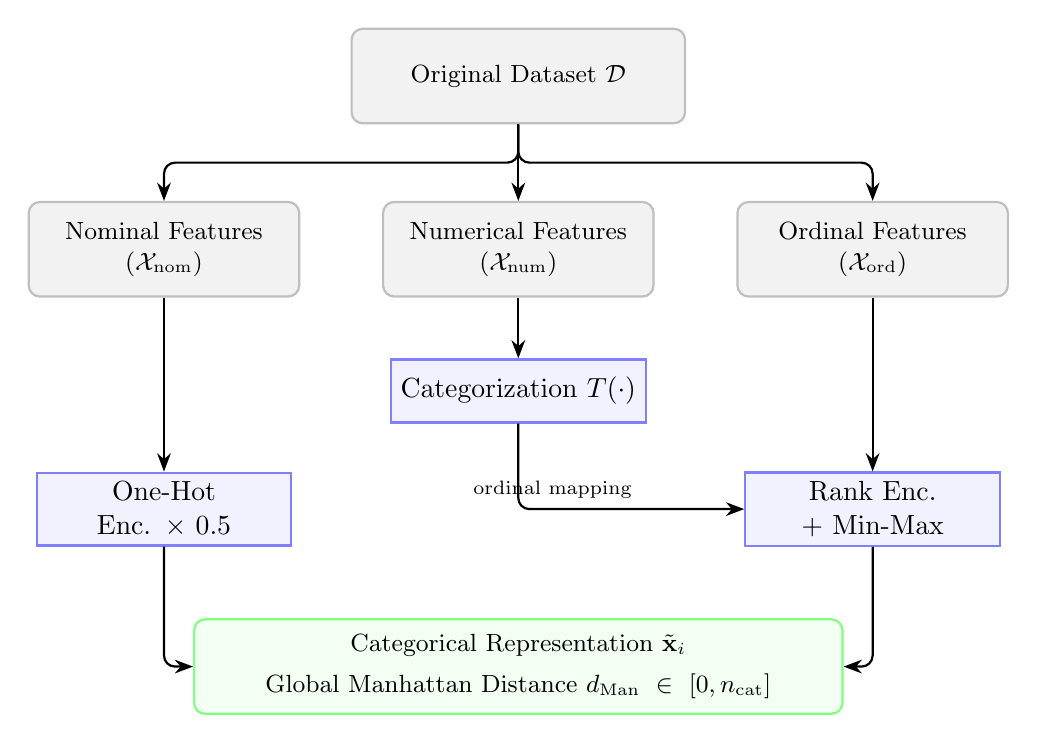
\begin{tikzpicture}[
    >=Stealth,
    box/.style={rectangle, draw=gray!50, fill=gray!10, thick, rounded corners, text width=3.2cm, align=center, minimum height=1.2cm, font=\small},
    op/.style={rectangle, draw=blue!50, fill=blue!5, thick, text width=3cm, align=center, minimum height=0.8cm, font=\footnotesize},
    final/.style={rectangle, draw=green!50, fill=green!5, thick, rounded corners, text width=8cm, align=center, minimum height=1.2cm, font=\small}
  ]
    \node[box, text width=4cm] (data) at (0,0) {Original Dataset $\mathcal{D}$};
    \node[box] (nom) at (-4.5,-2.2) {Nominal Features \\ ($\mathcal{X}_{\mathrm{nom}}$)};
    \node[box] (num) at (0,-2.2) {Numerical Features \\ ($\mathcal{X}_{\mathrm{num}}$)};
    \node[box] (ord) at (4.5,-2.2) {Ordinal Features \\ ($\mathcal{X}_{\mathrm{ord}}$)};
    \node[op] (cat) at (0,-4) {Categorization $T(\cdot)$};
    \node[op] (onehot) at (-4.5,-5.5) {One-Hot Enc. $\times$ 0.5};
    \node[op] (rank) at (4.5,-5.5) {Rank Enc. + Min-Max};
    \node[final] (global) at (0,-7.5) {Categorical Representation $\tilde{\mathbf{x}}_i$ \\[1ex] Global Manhattan Distance $d_{\mathrm{Man}} \in [0, n_{\mathrm{cat}}]$};
    \draw[->, thick, rounded corners] (data.south) -- (0,-1.1) -| (nom.north);
    \draw[->, thick] (data.south) -- (num.north);
    \draw[->, thick, rounded corners] (data.south) -- (0,-1.1) -| (ord.north);
    \draw[->, thick] (nom.south) -- (onehot.north);
    \draw[->, thick] (num.south) -- (cat.north);
    \draw[->, thick, rounded corners] (cat.south) |- node[above, font=\scriptsize, near end, xshift=-1cm] {ordinal mapping} (rank.west);
    \draw[->, thick] (ord.south) -- (rank.north);
    \draw[->, thick, rounded corners] (onehot.south) |- (global.west);
    \draw[->, thick, rounded corners] (rank.south) |- (global.east);
  \end{tikzpicture}
  \caption{Hybrid encoding workflow and feature space formalization.}
  \label{fig:hybrid-encoding}
\end{figure}

\section{BoCSoR: Method and Differences from Prior Work}
\label{sec:bocsor-method-prior-work}

This section first summarizes the BoCSoR method from which the present work takes inspiration, using the notation introduced in this thesis, and then describes how that method is adapted to the present setting and for which purpose it is used in the proposed pipeline.

\subsection{Original BoCSoR Method}

The methodological inspiration of this work is the approach presented in the paper \emph{From Local Counterfactuals to Global Feature Importance}~\cite{alfeo2023bocsor}. Since the original BoCSoR method is defined for purely continuous numerical features, in this subsection the feature space is temporarily restricted to its continuous numerical component, assuming $\mathcal{X} = \mathcal{X}_{\mathrm{num}}$. Consequently, each instance is explicitly treated as a fully numerical vector $\mathbf{x}^{\mathrm{num}}_i \in \mathcal{X}_{\mathrm{num}}$. Moreover, for simplicity and in line with the setting adopted in this thesis, the method is described in the binary-classification case $\mathcal{Y}=\{0,1\}$. The adaptation of this notion to the present setting, where all working features are categorical after the preprocessing step, is discussed in the next subsection.

BoCSoR belongs to a line of research in explainable artificial intelligence (XAI) that aims to explain the behavior of a trained classifier while treating it as a black box, that is, without relying on access to its internal structure. Let $\mathcal{D}=\{(\mathbf{x}^{\mathrm{num}}_i,y_i)\}_{i=1}^m$ denoted as the numerical dataset and let $f:\mathcal{X}_{\mathrm{num}}\rightarrow\mathcal{Y}$ be a generic classifier trained on the training set. From this perspective, the goal of the method is not to assess predictive performance on unseen data, but to explain the decision rule learned by the model from the data used during fitting. For this reason, the method is applied only to training instances, since these are the examples from which the classifier has learned the decision boundary that the explanation procedure aims to characterize. For a given class $y \in \mathcal{Y}$, let $\mathcal{D}_y$ denote the subset of training instances belonging to that class, defined as

\begin{equation}
  \mathcal{D}_y = \{ \mathbf{x}^{\mathrm{num}}_i \mid (\mathbf{x}^{\mathrm{num}}_i, y_i) \in \mathcal{D}, \; y_i = y \}.
\end{equation}

Since $\mathcal{Y}=\{0,1\}$, the set $\mathcal{D}_{1-y}$ analogously denotes the subset of training instances belonging to the opposite class. To make the two roles explicit in the remainder of this subsection, an instance belonging to the reference class is denoted by $\mathbf{x}^{\mathrm{num}, y}_i \in \mathcal{D}_y$, whereas an instance belonging to the opposite class is denoted by $\mathbf{x}^{\mathrm{num}, 1-y}_r \in \mathcal{D}_{1-y}$. Here, the superscripts $y$ and $1-y$ identify the class-specific subset to which the instance belongs, while the indices $i$ and $r$ distinguish generic elements within those two subsets.
Then, for each class $y \in \mathcal{Y}$ and for each instance $\mathbf{x}^{\mathrm{num}, y}_i \in \mathcal{D}_{y}$, all Euclidean distances $d_{\mathrm{eucl}}(\cdot \, , \cdot)$ from $\mathbf{x}^{\mathrm{num}, y}_i$ to all instances belonging to $\mathcal{D}_{1-y}$ are computed, namely:

\begin{equation}
  d_{\mathrm{eucl}}\!\left(\mathbf{x}^{\mathrm{num}, y}_i, \mathbf{x}^{\mathrm{num}, 1-y}_r\right), \qquad \forall \, r \in \{1, \ldots, |\mathcal{D}_{1-y}|\}.
\end{equation}

Among these distances, the minimum one $\delta_i^{y}$ for each instance $\mathbf{x}^{\mathrm{num}, y}_i \in \mathcal{D}_{y}$ is selected. Therefore, the minimum distance $\delta_i^{y}$ is defined as

\begin{equation}
  \delta_i^{y} = \min_{r \in \{1, \ldots, |\mathcal{D}_{1-y}|\}} d_{\mathrm{eucl}}\!\left(\mathbf{x}^{\mathrm{num}, y}_i, \mathbf{x}^{\mathrm{num}, 1-y}_r\right).
\end{equation}

Accordingly, for a fixed class $y \in \mathcal{Y}$, the set of such minimum distances is collected in

\begin{equation}
  \Delta_{y} = \left\{ \delta_i^{y} \, \middle| \, \mathbf{x}^{\mathrm{num}, y}_i \in \mathcal{D}_{y} \right\},
\end{equation}

so that $\Delta_y$ contains, for each instance in $\mathcal{D}_{y}$, the distance from that instance to the nearest instance of the opposite class. 

Let $\tau_p$ denote a threshold corresponding to a chosen empirical percentile computed on the set of distances $\Delta_{y}$. The set of \emph{boundary points} for a given class, denoted by $\mathcal{B}_y$, is defined as the collection of pairs $(\mathbf{x}^{\mathrm{num}, y}_i, \mathbf{x}^{\mathrm{num}, 1-y}_r)$, denoted here as boundary pairs, whose associated minimum distance $\delta_i^y \in \Delta_y$ is less than or equal to this threshold, namely:

\begin{equation}
  \mathcal{B}_y = \left\{ \left(\mathbf{x}^{\mathrm{num}, y}_i, \mathbf{x}^{\mathrm{num}, 1-y}_r\right) \, \middle| \, \delta_i^y \in \Delta_y,\; \delta_i^y \leq \tau_p \right\}.
\end{equation}

These are called boundary points precisely because they are the instances lying closest to the decision boundary; accordingly, they are also the instances for which the classifier is most uncertain, or equivalently, those on which it has the lowest confidence.  

Before continuing with the description of the method, it is useful to clarify what is meant by a \emph{counterfactual} in the literature~\cite{wachter2017counterfactual}. Let $\mathbf{x}^{\mathrm{num}, y}_i$ be a generic fully numerical continuous instance. Its corresponding counterfactual, denoted by $\mathbf{x}_i^{\mathrm{num}, 1-y, CF}$, is an instance belonging to the opposite class whose difference with respect to $\mathbf{x}^{\mathrm{num}, y}_i$, in terms of feature values, is minimal. 

Given a boundary pair $(\mathbf{x}^{\mathrm{num, y}}_i, \mathbf{x}^{\mathrm{num, 1-y}}_i)$, the method employed by BoCSoR to find the counterfactual $\mathbf{x}_i^{\mathrm{num}, 1-y, CF}$ of $\mathbf{x}^{\mathrm{num}, y}_i$ begins by drawing an imaginary line in the feature space between the two instances. This line is then sampled at 5 equally spaced points. Starting from the point closest to $\mathbf{x}^{\mathrm{num, 1-y}}_i$, the algorithm creates a new synthetic instance via linear interpolation. To determine whether this instance belongs to class $y$ or $1-y$, it is evaluated by the pre-trained classifier. 

If the predicted class for the new synthetic instance is $y$, then the original boundary instance $\mathbf{x}^{\mathrm{num, 1-y}}_i$ is chosen directly as the counterfactual. Otherwise, a new synthetic instance is generated and evaluated at the next point along the line. This process continues until an instance classified as class $y$ is found, at which point the synthetic instance generated in the immediately preceding step is selected as the counterfactual. If the process reaches the final point on the line before $\mathbf{x}^{\mathrm{num, y}}_i$ and predicts it to belong to class $1-y$, that final point is considered the counterfactual. 

In this way, BoCSoR successfully identifies an instance belonging to class $1-y$ (whether original or synthetic) that is closest to the instance $\mathbf{x}^{\mathrm{num, y}}_i$, which means that it has the smallest difference in feature values, namely, its corresponding counterfactual. For simplicity of notation, the generic $i$-th instance and its corresponding counterfactual are hereafter denoted by $\mathbf{x}^{\mathrm{num}}_i$ and $\mathbf{x}_i^{\mathrm{num}, CF}$, respectively. By repeating this procedure for each boundary pair, BoCSoR obtains all instance-counterfactual pairs $(\mathbf{x}^{\mathrm{num}}_i, \mathbf{x}_i^{\mathrm{num}, CF})$.

It is important to underline that this geometric interpolation relies on the continuous nature of the original feature space $\mathbb{R}^{n_{\mathrm{num}}}$, ensuring that synthetic points remain valid instances. The adaptation of this concept for discrete categorical spaces is detailed in the next subsection. A graphical illustration of the original BoCSoR boundary-point and counterfactual-refinement procedure in the continuous numerical setting is provided in Figure~\ref{fig:continuous-space-boundary}.

\begin{figure}[p]
  \centering
  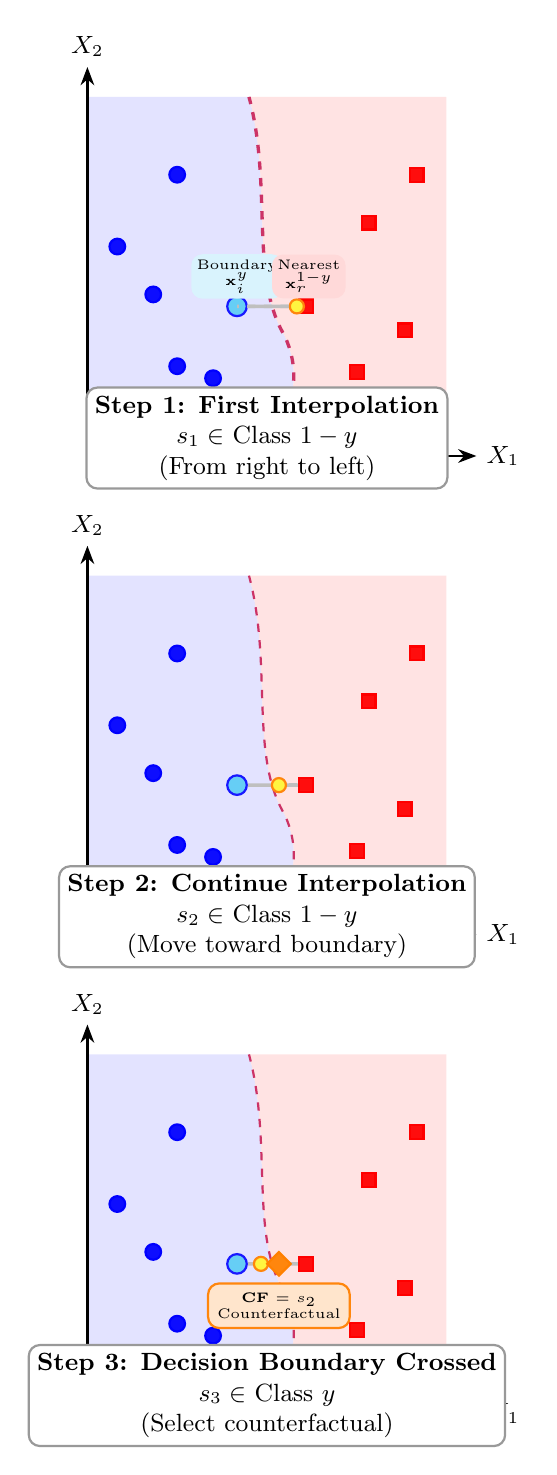
\begin{tikzpicture}[
    scale=0.76,
    axis/.style={thick, ->, >=Stealth},
    dot/.style={circle, inner sep=2pt},
    class0/.style={dot, fill=blue!95, draw=blue!100, thick},
    class1/.style={rectangle, inner sep=2.5pt, fill=red!95, draw=red!100, thick},
    boundary/.style={dot, fill=cyan!60, draw=blue!90, thick, inner sep=2.5pt},
    synth1/.style={dot, fill=yellow!75, draw=orange!95, thick, inner sep=1.8pt},
    synth2/.style={dot, fill=yellow!75, draw=orange!95, thick, inner sep=1.8pt},
    cfsynth/.style={diamond, fill=orange!95, draw=orange!100, thick, inner sep=2.2pt}
  ]
    \begin{scope}[yshift=0cm]
      \fill[blue!15, opacity=0.75]
      (0.5,0.5) -- (0.5,6.5) -- (3.2,6.5)
      .. controls (3.6,5) and (3.2,3.5) .. (3.8,2.5)
      .. controls (4.2,1.6) and (3.7,1.0) .. (3.4,0.5) -- cycle;
      \fill[red!15, opacity=0.75]
      (6.5,0.5) -- (6.5,6.5) -- (3.2,6.5)
      .. controls (3.6,5) and (3.2,3.5) .. (3.8,2.5)
      .. controls (4.2,1.6) and (3.7,1.0) .. (3.4,0.5) -- cycle;
      \draw[axis] (0.5,0.5) -- (7,0.5) node[right, font=\small] {$X_1$};
      \draw[axis] (0.5,0.5) -- (0.5,7) node[above, font=\small] {$X_2$};
      \draw[dashed, very thick, purple!80]
      (3.4,0.5)
      .. controls (3.7,1.0) and (4.2,1.6) .. (3.8,2.5)
      .. controls (3.2,3.5) and (3.6,5) .. (3.2,6.5);
      \node[class0] at (2,2) {};
      \node[class0] at (1,4) {};
      \node[class0] at (2,5.2) {};
      \node[class0] at (2.6,1.8) {};
      \node[class0] at (1.6,3.2) {};
      \node[class1] at (5.2,4.4) {};
      \node[class1] at (5.8,2.6) {};
      \node[class1] at (6,5.2) {};
      \node[class1] (nn1) at (4.15,3.0) {};
      \node[class1] at (5.0,1.9) {};
      \node[boundary] (bi) at (3,3) {};
      \draw[very thick, gray!50] (nn1) -- (bi);
      \node[synth1] (s1_p1) at (4.0,3.0) {};
      \draw[dashed, very thick, gray!50] (s1_p1) -- (3.0, 3.0);
      \node[font=\small, align=center, fill=white, inner sep=3pt, rounded corners, thick, draw=black!40] at (3.5, 0.8) {\textbf{Step 1: First Interpolation}\\$s_1 \in$ Class $1-y$\\(From right to left)};
      \node[font=\tiny, align=center, fill=cyan!15, rounded corners, inner sep=2pt] at (3, 3.5) {Boundary\\$\mathbf{x}_i^{y}$};
      \node[font=\tiny, align=center, fill=red!15, rounded corners, inner sep=2pt] at (4.2, 3.5) {Nearest\\$\mathbf{x}_r^{1-y}$};
    \end{scope}
    \begin{scope}[yshift=-8cm]
      \fill[blue!15, opacity=0.75]
      (0.5,0.5) -- (0.5,6.5) -- (3.2,6.5)
      .. controls (3.6,5) and (3.2,3.5) .. (3.8,2.5)
      .. controls (4.2,1.6) and (3.7,1.0) .. (3.4,0.5) -- cycle;
      \fill[red!15, opacity=0.75]
      (6.5,0.5) -- (6.5,6.5) -- (3.2,6.5)
      .. controls (3.6,5) and (3.2,3.5) .. (3.8,2.5)
      .. controls (4.2,1.6) and (3.7,1.0) .. (3.4,0.5) -- cycle;
      \draw[axis] (0.5,0.5) -- (7,0.5) node[right, font=\small] {$X_1$};
      \draw[axis] (0.5,0.5) -- (0.5,7) node[above, font=\small] {$X_2$};
      \draw[dashed, thick, purple!80]
      (3.4,0.5)
      .. controls (3.7,1.0) and (4.2,1.6) .. (3.8,2.5)
      .. controls (3.2,3.5) and (3.6,5) .. (3.2,6.5);
      \node[class0] at (2,2) {};
      \node[class0] at (1,4) {};
      \node[class0] at (2,5.2) {};
      \node[class0] at (2.6,1.8) {};
      \node[class0] at (1.6,3.2) {};
      \node[class1] at (5.2,4.4) {};
      \node[class1] at (5.8,2.6) {};
      \node[class1] at (6,5.2) {};
      \node[class1] (nn2) at (4.15,3.0) {};
      \node[class1] at (5.0,1.9) {};
      \node[boundary] (bi2) at (3,3) {};
      \draw[very thick, gray!50] (nn2) -- (bi2);
      \draw[dashed, very thick, gray!50] (4.0,3.0) -- (3.7,3.0);
      \node[synth2] (s2_p2) at (3.7,3.0) {};
      \node[font=\small, align=center, fill=white, inner sep=3pt, rounded corners, thick, draw=black!40] at (3.5, 0.8) {\textbf{Step 2: Continue Interpolation}\\$s_2 \in$ Class $1-y$\\(Move toward boundary)};
    \end{scope}
    \begin{scope}[yshift=-16cm]
      \fill[blue!15, opacity=0.75]
      (0.5,0.5) -- (0.5,6.5) -- (3.2,6.5)
      .. controls (3.6,5) and (3.2,3.5) .. (3.8,2.5)
      .. controls (4.2,1.6) and (3.7,1.0) .. (3.4,0.5) -- cycle;
      \fill[red!15, opacity=0.75]
      (6.5,0.5) -- (6.5,6.5) -- (3.2,6.5)
      .. controls (3.6,5) and (3.2,3.5) .. (3.8,2.5)
      .. controls (4.2,1.6) and (3.7,1.0) .. (3.4,0.5) -- cycle;
      \draw[axis] (0.5,0.5) -- (7,0.5) node[right, font=\small] {$X_1$};
      \draw[axis] (0.5,0.5) -- (0.5,7) node[above, font=\small] {$X_2$};
      \draw[dashed, thick, purple!80]
      (3.4,0.5)
      .. controls (3.7,1.0) and (4.2,1.6) .. (3.8,2.5)
      .. controls (3.2,3.5) and (3.6,5) .. (3.2,6.5);
      \node[class0] at (2,2) {};
      \node[class0] at (1,4) {};
      \node[class0] at (2,5.2) {};
      \node[class0] at (2.6,1.8) {};
      \node[class0] at (1.6,3.2) {};
      \node[class1] at (5.2,4.4) {};
      \node[class1] at (5.8,2.6) {};
      \node[class1] at (6,5.2) {};
      \node[class1] (nn3) at (4.15,3.0) {};
      \node[class1] at (5.0,1.9) {};
      \node[boundary] (bi3) at (3,3) {};
      \draw[very thick, gray!50] (nn3) -- (bi3);
      \draw[dashed, very thick, gray!50] (3.7,3.0) -- (3.4,3.0);
      \node[synth2] (s3_p3) at (3.4,3.0) {};
      \node[cfsynth] (s2_cf) at (3.7,3.0) {};
      \node[font=\small, align=center, fill=white, inner sep=3pt, rounded corners, thick, draw=black!40] at (3.5, 0.8) {\textbf{Step 3: Decision Boundary Crossed}\\$s_3 \in$ Class $y$\\(Select counterfactual)};
      \node[font=\tiny, align=center, draw=orange!95, rounded corners, fill=orange!20, thick] at (3.7, 2.3) {\textbf{CF} = $s_2$\\Counterfactual};
    \end{scope}
  \end{tikzpicture}
  \caption{Iterative process of the original BoCSoR method for finding synthetic counterfactuals. Panel 1 shows the first synthetic instance $s_1$ classified as class $1-y$. Panel 2 shows the second synthetic instance $s_2$, also classified as class $1-y$. Panel 3 shows the third synthetic instance $s_3$ classified as class $y$, triggering the selection of $s_2$ as the synthetic counterfactual $\mathbf{x}_i^{\mathrm{num},CF}$ closest to the boundary instance $\mathbf{x}_i^{\mathrm{num},y}$.}
  \label{fig:continuous-space-boundary}
\end{figure}

Considering an instance--counterfactual pair $(\mathbf{x}^{\mathrm{num}}_i, \mathbf{x}_i^{\mathrm{num}, CF})$ obtained through the procedure described above, to assess the importance of each feature index $j$ for the classification of $\mathbf{x}^{\mathrm{num}}_i$, BoCSoR performs a perturbation step. During this step, the method iterates over all features $X_j$, modifying one feature at a time in the counterfactual in order to evaluate the corresponding importance. More precisely, for each feature $X_j$, the value $x_{ij}^{\mathrm{num}, CF}$ in $\mathbf{x}_i^{\mathrm{num}, CF}$ is temporarily replaced with the corresponding value $x_{ij}^{\mathrm{num}}$ observed in $\mathbf{x}^{\mathrm{num}}_i$, while the remaining feature values are left unchanged. Denoting by $\mathbf{x}_{i}^{\mathrm{num}, CF, j}$ the perturbed counterfactual obtained after replacing, in $\mathbf{x}_i^{\mathrm{num}, CF}$, the value $x_{ij}^{\mathrm{num}, CF}$ with $x_{ij}^{\mathrm{num}}$, the instance $\mathbf{x}_{i}^{\mathrm{num}, CF, j}$ is then classified again by the trained classifier. The perturbation step is performed for all instance--counterfactual pairs. The outcome of all perturbation steps is formalized using the indicator function $\mathbb{I}(\cdot)$ introduced in Section~\ref{sec:hybrid-encoding-distance}

\begin{equation}
  I_{ij} = \mathbb{I}\left(f(\mathbf{x}_{i}^{\mathrm{num}, CF, j}) = f(\mathbf{x}^{\mathrm{num}}_i)\right) \qquad \forall i \in [1, m], j \in [1, n_\mathrm{num}].
\end{equation}

Accordingly, $I_{ij}=1$ if replacing $x_{ij}^{\mathrm{num}, CF}$ with $x_{ij}^{\mathrm{num}}$ causes the modified counterfactual to switch its predicted class to match the original instance, and $I_{ij}=0$ otherwise. Equivalently, the value $x_{ij}^{\mathrm{num}}$ is recorded as relevant for instance $\mathbf{x}^{\mathrm{num}}_i$ exactly when $I_{ij}=1$. After this check, the original value of the feature in the counterfactual is restored before proceeding to the next feature. If the replacement does not induce a class change, that original value is restored immediately, and the analysis continues with the next feature.

The whole procedure from the identification of the boundary points up to the perturbation step is then repeated for the instances belonging to the opposite class, so that both directions of the comparison are examined separately. The reason is that the two directions of the comparison are not, in general, symmetric: if $\mathbf{x}^{\mathrm{num}}_j$ is selected as a counterfactual reference for $\mathbf{x}^{\mathrm{num}}_i$, it does not necessarily follow that $\mathbf{x}^{\mathrm{num}}_i$ is also the counterfactual reference for $\mathbf{x}^{\mathrm{num}}_j$. Therefore, the local geometry of the instance--counterfactual relation may differ depending on which class is taken as the reference class. 

Let $\mathcal{B}$ be defined as the set of all boundary points 

\begin{equation}
  \mathcal{B} = \mathcal{B}_y \cup \mathcal{B}_{1-y},
\end{equation}

and let $|\mathcal{B}| = |\mathcal{B}_y| + |\mathcal{B}_{1-y}|$ denote the total number of boundary instance pairs. For each feature index $j$, let $S_j$ denote the total number of class-switch events induced by perturbing feature $X_j$ across all tested boundary instances:

\begin{equation}
  S_j = \sum_{\mathbf{x}^{\mathrm{num}}_i \in \mathcal{B}_y} I_{ij} + \sum_{\mathbf{x}^{\mathrm{num}}_i \in \mathcal{B}_{1-y}} I_{ij}.
\end{equation}

Equivalently,

\begin{equation}
  S_j = \sum_{\mathbf{x}^{\mathrm{num}}_i \, \in \, \mathcal{B}} I_{ij}.
\end{equation}

The BoCSoR score associated with feature index $j$ is then defined as

\begin{equation}
  \mathrm{BoCSoR}_j = \frac{S_j}{|\mathcal{B}|}.
\end{equation}

Hence, $\mathrm{BoCSoR}_j \in [0,1]$ measures the proportion of boundary instances in $\mathcal{B}_0 \cup \mathcal{B}_1$ for which substituting $x_{ij}^{\mathrm{num}}$ is sufficient to induce the class switch under the substitution test. In the original BoCSoR method, the object retained at this stage is therefore the feature index $j$, rather than the specific value $x_{ij}^{\mathrm{num}}$ involved in the replacement. The closer $\mathrm{BoCSoR}_j$ is to $1$, the greater the ability of the values observed for feature index $j$ to determine the model outcome on their own, thereby indicating very high global relevance for the corresponding feature in the model decisions. Thus, the BoCSoR score serves as a \textit{feature importance metric}, quantifying each feature's capacity to influence the model's decisions.

\subsection{Adaptation to the Present Work}

BoCSoR is here adapted to a setting that differs substantially from that of the original method. After the preprocessing stage described in the section \ref{sec:feature-space-formalization}, the dataset is entirely categorical. Accordingly, the analysis no longer operates in a continuous numerical feature space, but on the categorical dataset

\begin{equation}
  \widetilde{\mathcal{D}} = \{(\tilde{\mathbf{x}}_i, y_i)\}_{i=1}^{m},
  \qquad \tilde{\mathbf{x}}_i \in \widetilde{\mathcal{X}},
  \qquad y_i \in \mathcal{Y}=\{0,1\}.
\end{equation}

Under the notation introduced above, each instance is represented as

\begin{equation}
  \tilde{\mathbf{x}}_i = (\tilde{x}_{i1},\dots,\tilde{x}_{i\mathrm{n_{cat}}}),
\end{equation}

where each component $\tilde{x}_{ij}$ denotes the category associated with feature $X_j$, and for each feature index $j$ the admissible categories belong to the set $\mathcal{C}_j$.

This change has an immediate consequence for the definition of proximity between instances. In the original BoCSoR method, distances are computed in a continuous numerical space by means of the Euclidean metric, which is denoted here by $d_{\mathrm{eucl}}(\cdot \, , \cdot)$. In the present setting, this choice is no longer appropriate because the instances under comparison are fully categorical. Therefore the distance is instead computed through the global Manhattan distance defined in Section~\ref{sec:hybrid-encoding-distance}, namely $d_{\mathrm{Man}}(\tilde{\mathbf{x}}_a,\tilde{\mathbf{x}}_b)$.

As in the original BoCSoR method, the analysis is carried out exclusively on the training set, since the goal is to explain the decision rule learned by the classifier from the data used during fitting. Furthermore, also in this case only correctly classified training instances are retained, because the counterfactual comparison is intended to characterize the local structure of the model around instances for which the predicted class coincides with the true ground-truth class. Accordingly, let $\widetilde{\mathcal{D}}_{\mathrm{train}} \subset \widetilde{\mathcal{D}}$ denote the training set. For each target class $y \in \mathcal{Y}=\{0,1\}$, the subset of its correctly classified training instances is defined as

\begin{equation}
  \widetilde{\mathcal{D}}_{y} = \{ \tilde{\mathbf{x}}_i \mid (\tilde{\mathbf{x}}_i, y_i) \in \widetilde{\mathcal{D}}_{\mathrm{train}}, \; y_i = y, \; f(\tilde{\mathbf{x}}_i) = y \}.
\end{equation}

Since $\mathcal{Y}=\{0,1\}$, the set $\widetilde{\mathcal{D}}_{1-y}$ analogously denotes the subset of correctly classified training instances belonging to the opposite class. To make the two roles explicit in the remainder of this subsection, an instance belonging to the reference class is denoted by $\tilde{\mathbf{x}}^{y}_i \in \widetilde{\mathcal{D}}_y$, whereas an instance belonging to the opposite class is denoted by $\tilde{\mathbf{x}}^{1-y}_r \in \widetilde{\mathcal{D}}_{1-y}$.

Then, for each class $y \in \mathcal{Y}$ and for each instance $\tilde{\mathbf{x}}^{y}_i \in \widetilde{\mathcal{D}}_{y}$, all Manhattan distances from $\tilde{\mathbf{x}}^{y}_i$ to all instances of the opposite class are computed:

\begin{equation}
  d_{\mathrm{Man}}\!\left(\tilde{\mathbf{x}}^{y}_i, \tilde{\mathbf{x}}^{1-y}_r\right), \qquad \forall \, r \in \{1, \ldots, |\widetilde{\mathcal{D}}_{1-y}|\}.
\end{equation}

Among these distances, the minimum one for each instance $\tilde{\mathbf{x}}^{y}_i \in \widetilde{\mathcal{D}}_{y}$ is denoted by $\widetilde{\delta}_i^{y}$ and is defined as

\begin{equation}
  \widetilde{\delta}_i^{y} = \min_{r \in \{1, \ldots, |\widetilde{\mathcal{D}}_{1-y}|\}} d_{\mathrm{Man}}\!\left(\tilde{\mathbf{x}}^{y}_i, \tilde{\mathbf{x}}^{1-y}_r\right).
\end{equation}

Accordingly, for a fixed class $y \in \mathcal{Y}$, the set of such minimum distances is collected in

\begin{equation}
  \widetilde{\Delta}_{y} = \left\{ \widetilde{\delta}_i^{y} \, \middle| \, \tilde{\mathbf{x}}^{y}_i \in \widetilde{\mathcal{D}}_{y} \right\}.
\end{equation}

Also in this case $\tau_p$ denote a threshold corresponding to a chosen empirical percentile computed on the set of distances $\widetilde{\Delta}_{y}$. The set of boundary points for a given class, denoted by $\widetilde{\mathcal{B}}_y$, is defined as the collection of pairs $(\tilde{\mathbf{x}}^{y}_i, \tilde{\mathbf{x}}^{1-y}_r)$ denoted here as boundary pairs, whose associated minimum distance $\widetilde{\delta}_i^{y} \in \widetilde{\Delta}_{y}$ is less than or equal to this
threshold, namely:

\begin{equation}
  \widetilde{\mathcal{B}}_y = \left\{ \left(\tilde{\mathbf{x}}^{y}_i, \tilde{\mathbf{x}}^{1-y}_r\right) \, \middle| \, \widetilde{\delta}_i^y \in \widetilde{\Delta}_y,\; \widetilde{\delta}_i^y \leq \tau_p \right\}.
\end{equation}

A graphical illustration of the boundary-point selection procedure in the fully categorical setting is provided in Figure~\ref{fig:categorized-space-boundary}.

\begin{figure}[htbp]
  \centering
  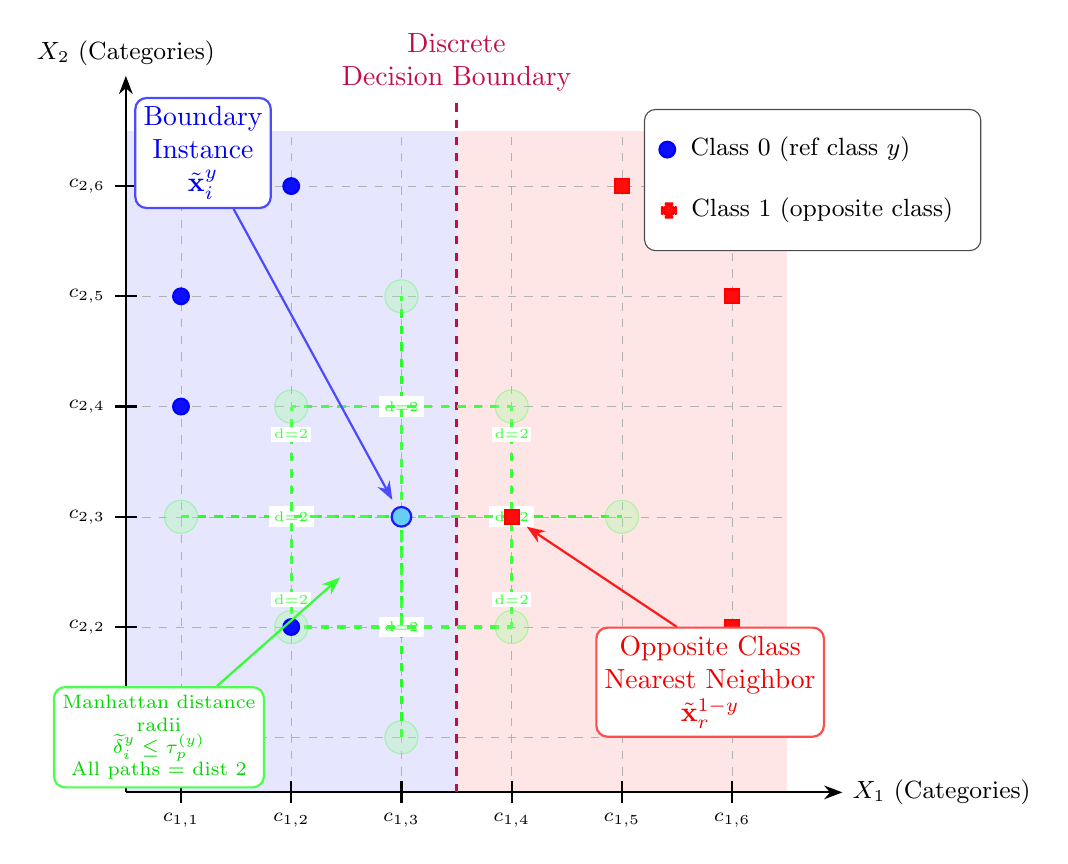
\begin{tikzpicture}[
    scale=1.4,
    axis/.style={thick, ->, >=Stealth},
    dot/.style={circle, inner sep=2pt},
    class0/.style={dot, fill=blue!95, draw=blue!100, thick},
    class1/.style={rectangle, inner sep=2.5pt, fill=red!95, draw=red!100, thick},
    boundary/.style={dot, fill=cyan!60, draw=blue!90, thick, inner sep=2.5pt},
    gridline/.style={gray!60, very thin, dashed}
  ]
    \fill[blue!15, opacity=0.65] (0.5,0.5) rectangle (3.5,6.5);
    \fill[red!15, opacity=0.65] (3.5,0.5) rectangle (6.5,6.5);
    \draw[gridline, step=1] (0.5,0.5) grid (6.5,6.5);
    \draw[axis] (0.5,0.5) -- (7,0.5) node[right, font=\small] {$X_1$ (Categories)};
    \draw[axis] (0.5,0.5) -- (0.5,7) node[above, font=\small] {$X_2$ (Categories)};
    \foreach \x in {1,2,3,4,5,6} {
      \draw[thick] (\x,0.4) -- (\x,0.6);
      \node[below=4pt, font=\scriptsize] at (\x,0.5) {$c_{1,\x}$};
    }
    \foreach \y in {1,2,3,4,5,6} {
      \draw[thick] (0.4,\y) -- (0.6,\y);
      \node[left=4pt, font=\scriptsize] at (0.5,\y) {$c_{2,\y}$};
    }
    \draw[dashed, very thick, purple!95] (3.5, 0.5) -- (3.5, 6.8) node[above, font=\footnotesize, align=center, fill=white, inner sep=2pt, rounded corners] {Discrete\\Decision Boundary};
    \draw[dashed, very thick, green!85] (3, 3) -- (3, 5) node[pos=0.5, font=\tiny, fill=white, inner sep=2pt] {d=2};
    \draw[dashed, very thick, green!85] (3, 1) -- (3, 3) node[pos=0.5, font=\tiny, fill=white, inner sep=2pt] {d=2};
    \draw[dashed, very thick, green!85] (3, 3) -- (5, 3) node[pos=0.5, font=\tiny, fill=white, inner sep=2pt] {d=2};
    \draw[dashed, very thick, green!85] (1, 3) -- (3, 3) node[pos=0.5, font=\tiny, fill=white, inner sep=2pt] {d=2};
    \draw[dashed, very thick, green!75] (3, 3) -- (3, 4) -- (4, 4);
    \draw[dashed, very thick, green!75] (3, 3) -- (4, 3) -- (4, 4) node[pos=0.75, font=\tiny, fill=white, inner sep=1pt] {d=2};
    \draw[dashed, very thick, green!75] (3, 3) -- (4, 3) -- (4, 2) node[pos=0.75, font=\tiny, fill=white, inner sep=1pt] {d=2};
    \draw[dashed, very thick, green!75] (3, 3) -- (3, 2) -- (4, 2);
    \draw[dashed, very thick, green!75] (3, 3) -- (2, 3) -- (2, 2) node[pos=0.75, font=\tiny, fill=white, inner sep=1pt] {d=2};
    \draw[dashed, very thick, green!75] (3, 3) -- (3, 2) -- (2, 2);
    \draw[dashed, very thick, green!75] (3, 3) -- (2, 3) -- (2, 4) node[pos=0.75, font=\tiny, fill=white, inner sep=1pt] {d=2};
    \draw[dashed, very thick, green!75] (3, 3) -- (3, 4) -- (2, 4);
    \foreach \pt in {(3,5), (3,1), (5,3), (1,3), (4,4), (4,2), (2,2), (2,4)} 
    {
      \draw[green!85, fill=green!40, opacity=0.3] \pt circle (0.15);
    }
    \node[class0] at (2,2) {};
    \node[class0] at (1,4) {};
    \node[class0] at (2,6) {};
    \node[class0] at (1,5) {};
    \node[class1] (nn1) at (4,3) {};
    \node[class1] at (6,5) {};
    \node[class1] at (5,6) {};
    \node[class1] at (6,2) {};
    \node[boundary] (bi) at (3,3) {};
    \draw[->, >=Stealth, shorten >=3pt, thick, red!90] (5.5, 2) -- (nn1);
    \node[font=\footnotesize, red!95!black, align=center, fill=white, inner sep=3pt, rounded corners, thick, draw=red!70] at (5.8, 1.5) {Opposite Class\\Nearest Neighbor\\$\tilde{\mathbf{x}}^{1-y}_{r}$};
    \node[font=\footnotesize, blue!95!black, align=center, fill=white, inner sep=3pt, rounded corners, thick, draw=blue!70] (lblBI) at (1.2, 6.3) {Boundary\\Instance\\$\tilde{\mathbf{x}}^{y}_i$};
    \draw[->, >=Stealth, shorten >=3pt, thick, blue!70] (lblBI) -- (bi);
    \node[font=\scriptsize, green!85!black, align=center, fill=white, inner sep=3pt, rounded corners, thick, draw=green!70] (lblDist) at (0.8, 1) {Manhattan distance\\radii\\$\widetilde{\delta}_{i}^{y} \leq \tau_p^{(y)}$\\All paths = dist 2};
    \draw[->, >=Stealth, shorten >=3pt, thick, green!80] (lblDist) -- (2.5, 2.5);
    \matrix [draw=black!70, fill=white, rounded corners, below right, font=\small, inner sep=5pt, row sep=3pt] at (5.2, 6.7) {
      \node[class0, label=right:{Class $0$ (ref class $y$)}] {}; \\
      \node[class1, label=right:{Class $1$ (opposite class)}] {}; \\
    };
  \end{tikzpicture}
  \caption{Schematic representation of the discrete categorical feature space. The boundary instance $\tilde{\mathbf{x}}^{y}_i$ is identified by computing Manhattan distances to all opposite-class instances. Green dashed lines with increased thickness indicate the Manhattan distance metric paths at multiple distance levels within the threshold $\widetilde{\delta}_{i}^{y} \leq \tau_p^{(y)}$, defining the boundary region in the discrete grid. The boundary instance of the opposite class $\tilde{\mathbf{x}}^{1-y}_{r}$ is selected as a potential counterfactual within this distance threshold.}
  \label{fig:categorized-space-boundary}
\end{figure}

After this step, one must address the second fundamental consequence of the present setting, regarding the generation of intermediate instances. In the original BoCSoR method, interpolation is meaningful because the feature space is continuous, so points lying on the line segment between an instance and its counterfactual remain well-defined elements of the space. In the present setting, by contrast, the feature space is fully categorical and inherently discrete.  Since interpolation is not suitable in this setting, given an instance $\tilde{\mathbf{x}}_i$, its counterfactual $\tilde{\mathbf{x}}^{CF}_i$ is defined simply as the nearest instance belonging to the opposite class.
In the fully categorical setting considered in this work, relying on a single nearest opposite-class instance is not always sufficient. Because distances are discrete, the nearest neighbor may reflect only one specific and possibly unstable way of crossing the decision boundary, and perturbing the associated features does not necessarily provide a robust explanation of the class-change mechanism. For this reason, the $k$ nearest opposite-class instances are considered as the $k$ counterfactuals of a considered instance, so as to obtain a more stable and representative description of the local decision region. In particular, relying on an ensemble of multiple neighbors helps absorb the variance naturally introduced by the discretization of the feature space, thereby providing a more robust estimate of the local decision boundary.

Specifically, fixing a reference class $y \in \mathcal{Y}$, for each instance $\tilde{\mathbf{x}}_i \in \widetilde{\mathcal{D}}_y$, the method identifies its $k$ nearest counterfactuals of the opposite class $\widetilde{\mathcal{D}}_{1-y}$, where $k$ is a configurable parameter of the analysis. Formally, for a given $k$, the $k$ counterfactuals in $\widetilde{\mathcal{D}}_{1-y}$ to $\tilde{\mathbf{x}}_i$, not necessarily in $\mathcal{B}_{1-y}$, are denoted by

\begin{equation}
  \tilde{\mathbf{x}}_{i,1}^{CF},\; \tilde{\mathbf{x}}_{i,2}^{CF},\; \dots,\; \tilde{\mathbf{x}}_{i,k}^{CF}.
\end{equation}

They are ordered by increasing Manhattan distance, i.e.,

\begin{equation}
  d_{\mathrm{Man}}(\tilde{\mathbf{x}}_i, \tilde{\mathbf{x}}_{i,1}^{CF}) \leq d_{\mathrm{Man}}(\tilde{\mathbf{x}}_i, \tilde{\mathbf{x}}_{i,2}^{CF}) \leq \cdots \leq d_{\mathrm{Man}}(\tilde{\mathbf{x}}_i, \tilde{\mathbf{x}}_{i,k}^{CF}).
\end{equation}

In the present fully categorical setting, given an instance $\tilde{\mathbf{x}}_i$ and one of its counterfactuals $\tilde{\mathbf{x}}_{i,r}^{CF}$, with $r \in \{1,\dots,k\}$, the perturbation step consists in replacing, for each feature $X_j$, the category $\tilde{x}_{ij,r}^{CF}$ (i.e., the $j$-th component of $\tilde{\mathbf{x}}_{i,r}^{CF}$) with the corresponding category $\tilde{x}_{ij}$ observed in the instance $\tilde{\mathbf{x}}_i$, while leaving all other components unchanged. The result is called perturbed counterfactual and denoted by $\tilde{\mathbf{x}}_{i,r}^{CF,j}$.
If the perturbation produces a class change with respect to the original observed class of the counterfactual, namely, if $f(\tilde{\mathbf{x}}_{i,r}^{CF,j}) = f(\tilde{\mathbf{x}}_i)$, then, differently from the original BoCSoR method, which records only the feature $X_j$ as relevant, the present approach records the full feature-category pair $(X_j = \tilde{x}_{ij})$, with $\tilde{x}_{ij} \in \mathcal{C}_j$, as relevant for the explanation of the instance $\tilde{\mathbf{x}}_i$ with respect to its $r$-th counterfactual.

The presented method introduces an additional element with respect to the original BoCSoR method. At the end of the perturbation step for each instance $\tilde{\mathbf{x}}_i$, all relevant feature-category pairs for that instance are collected into a list, denoted by $\mathcal{L}_i$. Since the present approach considers $k$ counterfactuals for each instance, this list is obtained by taking the union, over all counterfactuals $r$ and all features $j$, of the pairs for which the substitution test induces a class switch:

\begin{equation}
  \mathcal{L}_i = \bigcup_{r=1}^{k}\; \left\{ (X_j = \tilde{x}_{ij}) \;\middle|\; j \in \{1,\dots,n_{\mathrm{cat}}\},\; f(\tilde{\mathbf{x}}_{i,r}^{CF,j}) = f(\tilde{\mathbf{x}}_i) \right\}.
\end{equation}

\noindent\textbf{Example (perturbation step).} Consider an instance $\tilde{\mathbf{x}}_i$ belonging to the class $\mathcal{D}_y$, with the following categorical features after preprocessing:

\begin{equation*}
  \begin{aligned}
    \tilde{\mathbf{x}}_i = (&\texttt{Age=Middle-aged}, \texttt{Education=Bachelors}, \\
    &\texttt{Occupation=Tech-support}, \texttt{Sex=Male}),
  \end{aligned}
\end{equation*}

its nearest counterfactuals is:
\begin{equation}
  \begin{aligned}
    \tilde{\mathbf{x}}_{i,1}^{CF} = (\texttt{Age}=\texttt{Senior}, \texttt{Education}=\texttt{Masters}, \\ 
    \texttt{Occupation}=\texttt{Prof-specialty}, \texttt{Sex}=\texttt{Male}).
  \end{aligned}
\end{equation}

The perturbation step tests each feature in turn. For example, when perturbing the Education feature:

\begin{equation}
  \begin{aligned}
    \tilde{\mathbf{x}}_{i,1}^{CF,\texttt{Edu}} = (\texttt{Age}=\texttt{Senior}, \texttt{Education}=\texttt{Bachelors},\\ 
    \texttt{Occupation}=\texttt{Prof-specialty}, \texttt{Sex}=\texttt{Male}).
  \end{aligned}
\end{equation}

If $f(\tilde{\mathbf{x}}_{i,1}^{CF,\texttt{Edu}}) = f(\tilde{\mathbf{x}}_i)$, then the feature-category pair $(\texttt{Education}=\texttt{Bachelors})$ is recorded as relevant. Supposing that it is the only relevant feature-category pair with respect to the closest counterfactual, the local explanation list for $\tilde{\mathbf{x}}_i$ becomes

\begin{equation}
  \begin{aligned}
    \mathcal{L}_i = \{(\texttt{Education}=\texttt{Bachelors})\}.
  \end{aligned}
\end{equation}

Similarly, given the second closest counterfactual $\tilde{\mathbf{x}}_{i,2}^{CF}$

\begin{equation}
  \begin{aligned}
    \tilde{\mathbf{x}}_{i,2}^{CF,\texttt{Occ}} = (\texttt{Age}=\texttt{Senior}, \texttt{Education}=\texttt{Masters},\\
    \texttt{Occupation}=\texttt{Tech-support}, \texttt{Sex}=\texttt{Male}),
  \end{aligned}
\end{equation}

perturbing the $\texttt{Occupation}$ feature yields $f(\tilde{\mathbf{x}}_{i,2}^{CF,\texttt{Occ}}) = f(\tilde{\mathbf{x}}_i)$, making $(\texttt{Occupation}=\texttt{Tech-support})$ relevant. So the local explanation list for $\tilde{\mathbf{x}}_i$ becomes

\begin{equation}
  \begin{aligned}
    \mathcal{L}_i = \{(\texttt{Education}=\texttt{Bachelors}), (\texttt{Occupation}=\texttt{Tech-support})\}.
  \end{aligned}
\end{equation}

After testing all features and all $k$ counterfactuals, the local explanation list becomes

\begin{equation}
  \begin{aligned}
    \mathcal{L}_i = \{(\texttt{Education}=\texttt{Bachelors}),\\ 
    (\texttt{Occupation}=\texttt{Tech-support}),\\ 
    (\texttt{Age}=\texttt{Middle-aged})\},
  \end{aligned}
\end{equation}

capturing the specific feature-category combinations considered relevant for the local explanation of the model's decision on $\tilde{\mathbf{x}}_i$ with respect to its $k$ nearest counterfactuals.

The analysis is conducted separately in the two directions, exactly as in the original formulation. That is, instances are first analyzed in $\widetilde{\mathcal{D}}_{0}$ with counterfactual references searched in $\widetilde{\mathcal{D}}_{1}$, and the roles of the two classes are then reversed. This distinction remains important because the counterfactual relation is not symmetric: if an instance from class $1$ is the closest counterfactual to an instance from class $0$, the converse need not have the same local relevance under the adopted distance and with respect to the learned decision boundary. Analyzing the two directions separately therefore preserves the asymmetric local geometry of the classification problem within the categorical setting.

These lists $\mathcal{L}_i$ represent the local explanations for each point near the decision boundary. By collecting these pairs across all instances in $\widetilde{\mathcal{B}}_0 \cup \widetilde{\mathcal{B}}_1$, it becomes possible to analyze which specific categories (e.g., "Occupation = Tech-support") are most frequently responsible for the model's decisions. This approach allows for a granular and semantically meaningful global importance analysis, as it directly links the relevance of a feature to the specific categories it assumes in the dataset.

To synthesize the local findings into a broader perspective, the collection of all explanation lists obtained from the boundary instances is defined as:
\begin{equation}
  \mathcal{E} = \{ \mathcal{L}_i \mid \tilde{\mathbf{x}}_i \in \widetilde{\mathcal{B}}_0 \cup \widetilde{\mathcal{B}}_1 \} \qquad \forall i \in [1, m].
\end{equation}

This set $\mathcal{E}$ serves as the primary data structure for the global interpretation of the model. By aggregating the feature-category pairs contained in each $\mathcal{L}_i$, it is possible to identify recurring patterns and determine which specific categories across the entire feature space have the most significant impact on the classifier's behavior. This collective representation effectively bridges the gap between local counterfactual analysis and global model transparency, providing a comprehensive map of the decision logic within the categorical setting.

The complete procedure described above is summarized in Algorithm~\ref{alg:bocsor-adapted}.

\begin{algorithm}[H]
  \caption{Adapted BoCSoR for Categorical Data}\label{alg:bocsor-adapted}
  \begin{algorithmic}[1]
    \Statex \textbf{Input:}
    \Statex \quad $\widetilde{\mathcal{D}}_{\mathrm{train}}$: Training dataset with fully categorical features
    \Statex \quad $f$: Predictive classification model (black-box)
    \Statex \quad $p$: Percentile to define the boundary threshold $\tau$
    \Statex \quad $k$: Number of neighbors to extract candidate counterfactuals
    \Statex \textbf{Output:}
    \Statex \quad $\mathcal{E}$: Set of local explanations (one list $\mathcal{L}_i$ of relevant feature-category pairs per boundary instance)
    \Procedure{AdaptedBoCSoR}{$\widetilde{\mathcal{D}}_{\mathrm{train}},\, f,\, p,\, k$}
      \State $\mathcal{E} \gets \emptyset$ \Comment{Initialize the final set of local explanations}
      \For{$y \in \{0,1\}$}
        \State $\widetilde{\mathcal{D}}_y \gets$ correctly classified training instances with label $y$
        \State $\textit{nearestDist} \gets$ empty map \Comment{Initialize distance map}
        \For{$\tilde{\mathbf{x}} \in \widetilde{\mathcal{D}}_y$}
          \State $\textit{nearestDist}[\tilde{\mathbf{x}}] \gets \min_{\tilde{\mathbf{x}}' \in \widetilde{\mathcal{D}}_{1-y}} d_{\mathrm{Man}}(\tilde{\mathbf{x}}, \tilde{\mathbf{x}}')$ \Comment{Distance to closest opposite class instance}
        \EndFor
        \State $\tau \gets p$-th percentile of $\textit{nearestDist}$ \Comment{Compute boundary threshold}
        \State $\widetilde{\mathcal{B}}_y \gets \{\, \tilde{\mathbf{x}} \in \widetilde{\mathcal{D}}_y : \textit{nearestDist}[\tilde{\mathbf{x}}] \leq \tau \,\}$ \Comment{Collect boundary points}
        \For{$\tilde{\mathbf{x}}_i \in \widetilde{\mathcal{B}}_y$}
          \State $\textit{cfs} \gets$ $k$ nearest neighbours of $\tilde{\mathbf{x}}_i$ in $\widetilde{\mathcal{D}}_{1-y}$ under $d_{\mathrm{Man}}$ \Comment{Find candidate counterfactuals}
          \State $\mathcal{L}_i \gets \emptyset$ \Comment{Initialize list of feature-category pairs for $\tilde{\mathbf{x}}_i$}
          \For{$\tilde{\mathbf{x}}^{CF} \in \textit{cfs}$}
            \For{$j \in \{1, \ldots, n_{\mathrm{cat}}\}$}
              \State $\tilde{\mathbf{x}}' \gets \Call{Replace}{\tilde{\mathbf{x}}^{CF},\, j,\, \tilde{x}_{ij}}$ \Comment{Swap feature $j$ with the original category}
              \If{$f(\tilde{\mathbf{x}}') = f(\tilde{\mathbf{x}}_i)$} \Comment{Check if predicted class flips to the original}
                \State $\mathcal{L}_i \gets \mathcal{L}_i \cup \{(X_j = \tilde{x}_{ij})\}$ \Comment{Add relevant feature-category pair to the list}
              \EndIf
            \EndFor
          \EndFor
          \State $\mathcal{E} \gets \mathcal{E} \cup \{\mathcal{L}_i\}$ \Comment{Store the list of relevant feature-category pairs for $\tilde{\mathbf{x}}_i$}
        \EndFor
      \EndFor
      \State \Return $\mathcal{E}$
    \EndProcedure
  \end{algorithmic}
\end{algorithm}

\section{Association Rule Mining: Concepts and Foundations}
\label{sec:arm-foundations}

As discussed in the previous section, the adapted BoCSoR method provides a list $\mathcal{L}_i$ of relevant feature-category pairs for each boundary instance. To observe how combinations of these features influence the model's overall decisions, Association Rule Mining (ARM) is applied to the collection $\mathcal{E}$ of such lists. Before describing the analysis itself, this section introduces the foundational concepts of ARM, which are then specialized to the setting of this thesis.
Association Rule Mining is a data-mining technique for discovering relationships and patterns hidden within large transactional datasets. The method originated in the context of \emph{market basket analysis}~\cite{agrawal1994fast}, where the goal was to understand customer purchasing behavior by identifying which products tend to be bought together. Although ARM was initially developed for retail applications, its principles and algorithms have proven broadly applicable across diverse domains, including recommendation systems, web usage mining, and, as in the present work, model interpretability~\cite{han2000mining}.

\subsection{Origin: Market Basket Analysis}

In the classic market basket analysis scenario, a retailer maintains a transaction database where each entry records the items (products) purchased by a customer in a single shopping visit. The fundamental question driving this analysis concerns which items tend to be purchased together. Understanding such patterns allows retailers to optimize store layouts, design targeted promotions, and improve product recommendations. For instance, a retailer might discover that customers who buy bread and milk frequently also buy eggs, revealing a strong association among these products.

\subsection{Itemsets, Transactions, and Association Rules}

The foundational concepts of Association Rule Mining are \emph{itemsets} and \emph{transactions}. Formally, let $I = \{i_1, i_2, \dots, i_n\}$ be the universe of all available items, such as $I = \{\texttt{bread}, \texttt{milk}, \texttt{eggs}, \texttt{lemon}, \texttt{cheese}, \dots\}$. An \emph{itemset} is any subset $A \subseteq I$. An itemset containing $k$ items is typically referred to as a $k$-itemset. For example, $\{\texttt{bread}, \texttt{milk}\}$ is a 2-itemset, while $\{\texttt{eggs}\}$ is a 1-itemset.

An \emph{association rule} is an implication of the form $A \Rightarrow B$, where $A$ and $B$ are disjoint itemsets (i.e., $A \cap B = \emptyset$). The rule $A \Rightarrow B$ suggests that transactions containing the items in $A$ are likely to contain the items in $B$ as well. In the previous example, a possible association rule is $\{\texttt{bread}, \texttt{milk}\} \Rightarrow \{\texttt{eggs}\}$, indicating that customers who purchase bread and milk are likely to purchase eggs too.

A \emph{transaction} $T$ is a non-empty subset of items from $I$ (i.e., $T \subseteq I$), representing a specific purchase event. For example, $T = \{\texttt{bread}, \texttt{milk}, \texttt{eggs}\}$.

A \emph{transaction database} $\mathcal{D}$ is a collection of these transactions, denoted as $\mathcal{D} = \{T_1, T_2, \dots, T_q\}$, where each $T_k$ is uniquely identified by a transaction identifier (TID). An example database might be:

\begin{equation*}
  \begin{aligned}
    \mathcal{D} = \{&\{\texttt{bread}, \texttt{milk}, \texttt{eggs}\}, \{\texttt{milk}, \texttt{cheese}\},\\
    &\{\texttt{eggs}, \texttt{cheese}, \texttt{lemon}\}, \{\texttt{butter}\}, \dots \}.
  \end{aligned}
\end{equation*}

Consider a supermarket transaction database with five transactions recording customer purchases:

\begin{table}[H]
  \centering
  \renewcommand{\arraystretch}{1.2}
  \begin{tabularx}{\textwidth}{>{\centering\arraybackslash}p{0.16\textwidth}|>{\raggedright\arraybackslash}X}
    \toprule
    \textbf{Transaction ID} & \textbf{Items Purchased} \\
    \midrule
    $\text{TID}_1$ & \texttt{bread}, \texttt{milk}, \texttt{eggs}, \texttt{butter} \\
    $\text{TID}_2$ & \texttt{bread}, \texttt{milk}, \texttt{eggs} \\
    $\text{TID}_3$ & \texttt{milk}, \texttt{eggs}, \texttt{cheese} \\
    $\text{TID}_4$ & \texttt{bread}, \texttt{butter} \\
    $\text{TID}_5$ & \texttt{bread}, \texttt{milk}, \texttt{eggs}, \texttt{butter}, \texttt{cheese} \\
    \bottomrule
  \end{tabularx}
  \caption{Example transaction database for market basket analysis.}
  \label{tab:market-basket-example}
\end{table}

Inspecting this database, one can observe that \texttt{bread}, \texttt{milk}, and \texttt{eggs} are frequently purchased together, while \texttt{cheese} appears less often. This suggests potential correlations between \texttt{bread}, \texttt{milk}, and \texttt{eggs}, and that \texttt{cheese} is purchased without being strictly linked to other items. The goal of ARM is to systematically analyze such databases to discover all significant underlying patterns and correlations.

\subsection{Metrics}

The quality and significance of an association rule are evaluated using several metrics, of which the most important are support, confidence, and lift.

\paragraph{Support of an itemset.} The \emph{support} of an itemset $A$, denoted $\mathrm{supp}(A)$, is defined as the fraction of transactions in $\mathcal{D}$ that contain $A$:

\begin{equation}
  \mathrm{supp}(A) = \frac{|\{T_k \in \mathcal{D} \mid A \subseteq T_k\}|}{|\mathcal{D}|}.
\end{equation}

An itemset $A$ is called \emph{frequent} if $\mathrm{supp}(A) \geq \sigma$, where $\sigma$ is a user-defined minimum support threshold. The problem of finding all frequent itemsets is a central task in ARM, with efficient algorithms such as Apriori~\cite{agrawal1994fast} and FP-Growth~\cite{han2000mining} developed to solve it.

\paragraph{Example (support of an itemset).} Considering the universe of items $I = \{\texttt{bread}, \texttt{milk}, \texttt{eggs}, \texttt{butter}, \texttt{cheese}\}$, the support of various itemsets can be computed as follows:

\begin{itemize}
  \item $\mathrm{supp}(\{\texttt{bread}\}) = \frac{4}{5} = 0.80$, since \texttt{bread} appears \\ 
  in transactions $\text{TID}_1, \text{TID}_2, \text{TID}_4, \text{TID}_5$.
  \item $\mathrm{supp}(\{\texttt{milk}\}) = \frac{4}{5} = 0.80$, since \texttt{milk} appears\\
  in transactions $\text{TID}_1, \text{TID}_2, \text{TID}_3, \text{TID}_5$.
  \item $\mathrm{supp}(\{\texttt{eggs}\}) = \frac{4}{5} = 0.80$, since \texttt{eggs} appears\\
  in transactions $\text{TID}_1, \text{TID}_2, \text{TID}_3, \text{TID}_5$.
  \item $\mathrm{supp}(\{\texttt{butter}\}) = \frac{3}{5} = 0.60$, since \texttt{butter} appears\\
  in transactions $\text{TID}_1, \text{TID}_4, \text{TID}_5$.
  \item $\mathrm{supp}(\{\texttt{cheese}\}) = \frac{2}{5} = 0.40$, since \texttt{cheese} appears\\
  in transactions $\text{TID}_3, \text{TID}_5$.
  \item $\mathrm{supp}(\{\texttt{bread}, \texttt{milk}\}) = \frac{3}{5} = 0.60$, since both appear \\
  together in transactions $\text{TID}_1, \text{TID}_2, \text{TID}_5$.
  \item $\mathrm{supp}(\{\texttt{bread}, \texttt{milk}, \texttt{eggs}\}) = \frac{3}{5} = 0.60$, since all three appear\\
  together in transactions $\text{TID}_1, \text{TID}_2, \text{TID}_5$.
\end{itemize}

If a minimum support threshold $\sigma = 0.50$ is set, then the itemsets $\{\texttt{bread}\}$, $\{\texttt{milk}\}$, $\{\texttt{eggs}\}$, $\{\texttt{butter}\}$, $\{\texttt{bread}, \texttt{milk}\}$, and $\{\texttt{bread}, \texttt{milk}, \texttt{eggs}\}$ are all frequent, whereas $\{\texttt{cheese}\}$ with support $0.40$ would not be considered frequent under this threshold.

\paragraph{Support of a rule.} The support of a rule $A \Rightarrow B$ is the support of the itemset $A \cup B$:

\begin{equation}
  \mathrm{supp}(A \Rightarrow B) = \mathrm{supp}(A \cup B).
\end{equation}

This metric indicates the proportion of transactions in the database that contain both $A$ and $B$. A rule with high support indicates that the pattern is common in the database and potentially valuable for practical applications.

\paragraph{Example (support of a rule).} For the rule $\{\texttt{bread}, \texttt{milk}\} \Rightarrow \{\texttt{eggs}\}$, using the Table \ref{tab:market-basket-example}:

\begin{itemize}
  \item $\mathrm{supp}(\{\texttt{bread}, \texttt{milk}, \texttt{eggs}\}) = 0.60$, since all three items appear together in transactions $\text{TID}_1, \text{TID}_2, \text{TID}_5$.
\end{itemize}


\paragraph{Confidence of a rule.} The confidence of a rule $A \Rightarrow B$ is defined as:

\begin{equation}
  \mathrm{conf}(A \Rightarrow B) = \frac{\mathrm{supp}(A \cup B)}{\mathrm{supp}(A)}.
\end{equation}

This metric measures the \emph{strength} of the implication: it represents the probability that $B$ is purchased given that $A$ is purchased. A high confidence indicates a strong rule, meaning that whenever $A$ appears, $B$ is very likely to appear as well. Confidence values range from $0$ to $1$, where a confidence of $1$ indicates a perfect rule (i.e., whenever $A$ is present, $B$ is always present), and a confidence close to $0$ indicates a weak rule.

\paragraph{Example (confidence of a rule).} For the rule $\{\texttt{bread}, \texttt{milk}\} \Rightarrow \{\texttt{eggs}\}$, using the Table \ref{tab:market-basket-example}:

\begin{itemize}
  \item $\mathrm{conf}(\{\texttt{bread}, \texttt{milk}\} \Rightarrow \{\texttt{eggs}\}) = \frac{0.60}{0.60} = 1.0$, since the support of $\{\texttt{bread}, \texttt{milk}, \texttt{eggs}\}$ is $0.60$ and the support of $\{\texttt{bread}, \texttt{milk}\}$ is also $0.60$. This indicates a perfect rule: whenever customers purchase both \texttt{bread} and \texttt{milk}, they also purchase \texttt{eggs}.
\end{itemize}

\paragraph{Lift of a rule.} The lift of a rule $A \Rightarrow B$ is defined as:

\begin{equation}
  \mathrm{lift}(A \Rightarrow B) = \frac{\mathrm{conf}(A \Rightarrow B)}{\mathrm{supp}(B)}.
\end{equation}

Lift measures the \emph{correlation} between $A$ and $B$, specifically whether their co-occurrence is more frequent than expected if they were independent:

\begin{itemize}
  \item If $\mathrm{lift}(A \Rightarrow B) > 1$, then $A$ and $B$ are \emph{positively correlated}: the presence of $A$ increases the likelihood that $B$ is also present, beyond what would be expected by chance.
  \item If $\mathrm{lift}(A \Rightarrow B) < 1$, then $A$ and $B$ are \emph{negatively correlated}: the presence of $A$ decreases the likelihood that $B$ is also present.
  \item If $\mathrm{lift}(A \Rightarrow B) = 1$, then $A$ and $B$ are \emph{independent}: the presence of $A$ has no effect on the presence of $B$.
\end{itemize}

\paragraph{Example (lift of a rule).} For the rule $\{\texttt{bread}, \texttt{milk}\} \Rightarrow \{\texttt{eggs}\}$, using the Table \ref{tab:market-basket-example}:

\begin{itemize}
  \item $\mathrm{lift}(\{\texttt{bread}, \texttt{milk}\} \Rightarrow \{\texttt{eggs}\}) = \frac{1.0}{0.80} = 1.25$. This indicates a positive correlation: customers who buy \texttt{bread} and \texttt{milk} are $25\%$ more likely to buy \texttt{eggs} than a random customer.
\end{itemize}

\paragraph{Market basket example (negative correlation).} Another example is the rule $\{\texttt{butter}\} \Rightarrow \{\texttt{cheese}\}$, using the Table \ref{tab:market-basket-example}:

\begin{itemize}
  \item $\mathrm{supp}(\{\texttt{butter}, \texttt{cheese}\}) = \frac{1}{5} = 0.20$, since both items appear together only in transaction $\text{TID}_5$.
  \item $\mathrm{conf}(\{\texttt{butter}\} \Rightarrow \{\texttt{cheese}\}) = \frac{0.20}{0.60} = 0.33$, since \texttt{butter} appears in three transactions ($\text{TID}_1, \text{TID}_4, \text{TID}_5$), but only one of those transactions contains \texttt{cheese}.
  \item $\mathrm{lift}(\{\texttt{butter}\} \Rightarrow \{\texttt{cheese}\}) = \frac{0.33}{0.40} = 0.825$, since the support of \texttt{cheese} is $0.40$. This indicates a negative correlation: customers who buy \texttt{butter} are slightly less likely to buy \texttt{cheese} than a random customer.
\end{itemize}

\subsection{Application to Model Interpretability}

Instead of analyzing frequently purchased products, this thesis leverages the principles of ARM to assess which feature-category combinations are frequently relevant to the classifier's decisions, identifying recurring patterns in the model's decision logic.

In this setting, the set of explanation lists $\mathcal{E}$ is treated as a transaction database (e.g., $\mathcal{E} = \{\mathcal{L}_1, \mathcal{L}_2, \mathcal{L}_3, \mathcal{L}_4, \mathcal{L}_5\}$). A single list $\mathcal{L}_i \in \mathcal{E}$ is treated as a transaction, and each feature-category pair $(X_j = \tilde{x}_{ij})$ within that list is treated as an item. Formally, while $\mathcal{L}_i$ is conceptually introduced as a list of relevant explanations, in the context of Association Rule Mining it is strictly treated as a set of unique feature-category pairs. This structural assumption ensures that subset operations and ARM metrics, such as support and confidence, are rigorously well-defined without the ambiguity of duplicate items.

For example, if $\mathcal{L}_i = \{\texttt{Education}=\texttt{Bachelors}, \ \texttt{Occupation}=\texttt{Tech-support}, \ \texttt{Age}=\texttt{Middle-aged}\}$, then the transaction corresponding to $\mathcal{L}_i$ contains the items $\{\texttt{Education}=\texttt{Bachelors}\}$, $\{\texttt{Occupation}=\texttt{Tech-support}\}$, and $\{\texttt{Age}=\texttt{Middle-aged}\}$.

In this setting $A$ and $B$ are two disjoint itemsets consisting of feature-category pairs. An association rule $A \Rightarrow B$ in market basket analysis suggests that when the items of $A$ appear, $B$ are highly likely to appear as well. In this context, this means that if the feature-category pairs in $A$ are relevant to the model's decision, those in $B$ are also likely to be relevant. ARM thus identifies and quantifies the co-occurrence of specific feature-category pairs across the local explanations, revealing the underlying patterns that drive the model's predictions.

\paragraph{Example (transaction database of feature-category pairs).} Consider a simplified scenario where the adapted BoCSoR method has been applied to a set of boundary instances, yielding the following collection of explanation lists $\mathcal{E}$:

\begin{itemize}    
  \item $\mathcal{L}_1 = \{\texttt{Education}=\texttt{Bachelors}, \ \texttt{Occupation}=\texttt{Tech-support}, \ \texttt{Age}=\texttt{Middle-aged}\},$
  \item $\mathcal{L}_2 = \{\texttt{Education}=\texttt{Masters}, \ \texttt{Occupation}=\texttt{Prof-specialty}\},$
  \item $\mathcal{L}_3 = \{\texttt{Education}=\texttt{Bachelors}, \ \texttt{Occupation}=\texttt{Tech-support}, \ \texttt{Sex}=\texttt{Male}\},$
  \item $\mathcal{L}_4 = \{\texttt{Age}=\texttt{Senior}\},$
  \item $\mathcal{L}_5 = \{\texttt{Education}=\texttt{Bachelors}, \ \texttt{Occupation}=\texttt{Tech-support}, \\ \texttt{Age}=\texttt{Middle-aged}, \ \texttt{Sex}=\texttt{Male}\}.$
\end{itemize}

Each list $\mathcal{L}_i$ is treated as a transaction, and each feature-category pair within that list is treated as an item. The resulting transaction database $\mathcal{E}$ is summarized in Table~\ref{tab:feature-category-transactions}.

\begin{table}[H]
  \centering
  \renewcommand{\arraystretch}{1.3}
  \begin{tabularx}{\textwidth}{>{\centering\arraybackslash}p{0.16\textwidth}|>{\raggedright\arraybackslash}X}
    \toprule
    \textbf{Transaction ID} & \textbf{Feature-Category Pairs} \\
    \midrule
    $\mathcal{L}_1$ & Education=Bachelors, Occupation=Tech-support, Age=Middle-aged \\
    $\mathcal{L}_2$ & Education=Masters, Occupation=Prof-specialty \\
    $\mathcal{L}_3$ & Education=Bachelors, Occupation=Tech-support, Sex=Male \\
    $\mathcal{L}_4$ & Age=Senior \\
    $\mathcal{L}_5$ & Education=Bachelors, Occupation=Tech-support, Age=Middle-aged, Sex=Male \\
    \bottomrule
  \end{tabularx}
  \caption{Transaction database of feature-category pairs extracted from local explanations.}
  \label{tab:feature-category-transactions}
\end{table}

Inspecting the transaction database in Table~\ref{tab:feature-category-transactions}, several patterns emerge. The pair $(\texttt{Education}=\texttt{Bachelors})$ appears in three transactions ($\mathcal{L}_1, \mathcal{L}_3, \mathcal{L}_5$), as does $(\texttt{Occupation}=\texttt{Tech-support})$ in the same three transactions. This indicates a strong co-occurrence between these two feature-category pairs. In contrast, $(\texttt{Age}=\texttt{Senior})$ appears only in transaction $\mathcal{L}_4$, being less frequently associated with other pairs. Similarly, $(\texttt{Education}=\texttt{Masters})$ and $(\texttt{Occupation}=\texttt{Prof-specialty})$ appear together only in transaction $\mathcal{L}_2$, indicating a specialized pattern that differs from the dominant Bachelors--Tech-support combination. These observations suggest potential correlations between $(\texttt{Education}=\texttt{Bachelors})$ and $(\texttt{Occupation}=\texttt{Tech-support})$, while other combinations appear less systematic.

Support, confidence, and lift metrics are also used in this setting to evaluate association rules; however, their meanings change, as detailed in the following sections:

\paragraph{Support.} The support $\mathrm{supp}(A)$ measures the frequency of an itemset within $\mathcal{E}$:

\begin{equation}
  \mathrm{supp}(A) = \frac{|\{ \mathcal{L}_i \in \mathcal{E} \mid A \subseteq \mathcal{L}_i \}|}{|\mathcal{E}|}.
\end{equation}

A high support ensures that the identified pattern is not an outlier but a representative behavior of the model across a significant portion of the boundary instances. For a given rule $A \Rightarrow B$, the support is computed as the ratio of transactions containing both $A$ and $B$ over the total number of transactions. For a rule to be meaningful, both $A$ and $B$ must have sufficiently high support, ensuring that the rule is derived from a substantial number of instances.

\noindent\textbf{Example (support in model interpretability).} Referring to Table~\ref{tab:feature-category-transactions}, the support of various feature-category pairs can be computed as follows:

\begin{itemize}
  \item $\mathrm{supp}(\{\texttt{Education}=\texttt{Bachelors}\}) = \frac{3}{5} = 0.60$, since \path{Education=Bachelors} appears in transactions $\mathcal{L}_1$, $\mathcal{L}_3$, and $\mathcal{L}_5$.
  \item $\mathrm{supp}(\{\texttt{Occupation}=\texttt{Tech-support}\}) = \frac{3}{5} = 0.60$, since \path{Occupation=Tech-support} appears in transactions $\mathcal{L}_1$, $\mathcal{L}_3$, and $\mathcal{L}_5$.
  \item $\mathrm{supp}(\{\texttt{Age}=\texttt{Middle-aged}\}) = \frac{2}{5} = 0.40$, since \path{Age=Middle-aged} appears in transactions $\mathcal{L}_1$ and $\mathcal{L}_5$.
  \item $\mathrm{supp}(\{\texttt{Education}=\texttt{Bachelors}, \texttt{Occupation}=\texttt{Tech-support}\}) = \frac{3}{5} = 0.60$, since both appear together in transactions $\mathcal{L}_1$, $\mathcal{L}_3$, and $\mathcal{L}_5$.
\end{itemize}

\paragraph{Confidence.} The confidence $\mathrm{conf}(A \Rightarrow B)$ measures the strength of the inference:

\begin{equation}
  \mathrm{conf}(A \Rightarrow B) = \frac{\mathrm{supp}(A \cup B)}{\mathrm{supp}(A)}.
\end{equation}

This metric indicates how often $B$ is relevant when $A$ is relevant. A high confidence value suggests a strong association between the itemsets, indicating that the presence of $A$ is a reliable predictor of the presence of $B$ in the model's decision logic. High-confidence rules are more likely to represent meaningful feature interactions that the model relies on, rather than coincidental co-occurrences.

\noindent\textbf{Example (confidence in model interpretability).} Let
\[
  A = \{\texttt{Education}=\texttt{Bachelors}\}, \qquad B = \{\texttt{Occupation}=\texttt{Tech-support}\}.
\]
Using Table~\ref{tab:feature-category-transactions}, we obtain:

\begin{itemize}
  \item Support of the combined itemset: \[\mathrm{supp}(A \cup B) = 0.60.\]
  \item Support of the antecedent: \[\mathrm{supp}(A) = 0.60.\]
  \item Confidence: \[\mathrm{conf}(A \Rightarrow B) = \frac{0.60}{0.60} = 1.0.\]
\end{itemize}

A confidence of $1.0$ indicates that whenever \texttt{Education=Bachelors} appears in an explanation, \texttt{Occupation=Tech-support} is also present: in the model's decision logic, the \texttt{Bachelors} degree always co-occurs with a \texttt{Tech-support} occupation when explaining boundary instance decisions.

\paragraph{Lift.} The lift $\mathrm{lift}(A \Rightarrow B)$ measures the correlation between $A$ and $B$, specifically evaluating whether their co-occurrence is more frequent than expected under the assumption of independence:

\begin{equation}
  \mathrm{lift}(A \Rightarrow B) = \frac{\mathrm{conf}(A \Rightarrow B)}{\mathrm{supp}(B)}.
\end{equation}

\begin{itemize}
  \item If $\mathrm{lift}(A \Rightarrow B) > 1$, then $A$ and $B$ are positively correlated. The presence of $A$ increases the likelihood that $B$ is also relevant to the model's decision.
  \item If $\mathrm{lift}(A \Rightarrow B) < 1$, then $A$ and $B$ are negatively correlated: the presence of $A$ reduces the likelihood of $B$ being relevant.
  \item If $\mathrm{lift}(A \Rightarrow B) \approx 1$, then $A$ and $B$ are independent: the presence of $A$ does not affect the relevance of $B$.
\end{itemize}

\noindent\textbf{Example (lift in model interpretability).} Continuing with the same sets $A$ and $B$ from Table~\ref{tab:feature-category-transactions}, we obtain:

\begin{itemize}
  \item Confidence: \[\mathrm{conf}(A \Rightarrow B) = 1.0.\]
  \item Support of the consequent: \[\mathrm{supp}(B) = 0.60.\]
  \item Lift: \[\mathrm{lift}(A \Rightarrow B) = \frac{1.0}{0.60} \approx 1.67.\]
\end{itemize}

Since $\mathrm{lift} > 1$, these two feature-category pairs are positively correlated. A lift of $1.67$ means that $\{\texttt{Education}=\texttt{Bachelors}\}$ and $\{\texttt{Occupation}=\texttt{Tech-support}\}$ co-occur in the local explanations approximately $67\%$ more frequently than would be expected by chance. This above-chance co-occurrence indicates a meaningful synergy between these two feature-category pairs in the classifier's decision logic.

In this setting, a window $[1 - \epsilon, 1 + \epsilon]$ is considered around the baseline value of $\mathrm{lift}=1$, where $\epsilon$ is a small positive threshold. Rules with lift values falling within this range are considered to lack significant correlation and are therefore filtered out. This filtering process ensures that only meaningful insights into the model's decision logic are retained, helping to distinguish genuine feature dependencies from spurious associations.

\section{Hierarchical Association Rule Analysis}

Applying ARM directly to the collection of local explanations $\mathcal{E}$ poses two related difficulties. The first is combinatorial: with $n_{\mathrm{cat}}$ features and up to $p_j$ categories per feature, the number of possible feature-category pairs is $\sum_j p_j$, and the number of candidate itemsets of size $k$ grows as $\bigl(\sum_j p_j\bigr)^k$. Even modest values of $n_{\mathrm{cat}}$ yield a prohibitively large rule space.

The second difficulty is interpretive. Many rules that ARM would return as distinct are in fact different manifestations of the same underlying pattern. For instance, the rules $\{\texttt{Education}=\texttt{Bachelors}\} \Rightarrow \{\texttt{Occupation}=\texttt{Tech-support}\}$ and $\{\texttt{Education}=\texttt{Masters}\} \Rightarrow \{\texttt{Occupation}=\texttt{Prof-specialty}\}$ are reported as two independent rules by ARM, yet they both instantiate a single, coarser observation: that the features \texttt{Education} and \texttt{Occupation} tend to be jointly relevant for the model's decisions, regardless of which specific categories are involved. This means that in this setting it is possible to analyze how relevant features co-occur with one another and how combinations of these features represent decision patterns for the model, at two distinct levels of granularity: at the feature level and at the category level within the feature-category pair.

To address both difficulties, the analysis is organized into two levels of granularity:

\begin{itemize}
  \item The \emph{macroscopic level} discovers the \emph{macroscopic rules} in the transactions of $\mathcal{E}$, namely, rules containing only the \emph{feature} of each feature-category pair. This analysis considers only the feature and ignores category values in the transactions of feature-category pairs. It therefore observes whether and how features are jointly relevant in the model's decisions, providing an overview that abstracts from the specific categories involved. This analysis yields rules such as $\{\texttt{Education}\} \Rightarrow \{\texttt{Occupation}\}$, which state that the relevance of the feature \texttt{Education} is associated with the relevance of the feature \texttt{Occupation}, without specifying which categories of these features are involved.
  \item The \emph{microscopic level} discovers the \emph{microscopic rules} in the transactions of $\mathcal{E}$, namely, rules containing the full \emph{feature-category pair}. This analysis considers the full feature-category pairs, and it is based on the macroscopic rules produced in the macroscopic analysis. Given a macroscopic rule, the analysis at the microscopic level considers only transactions that contain categories in the feature-category pairs belonging to all features of the considered macroscopic rule. This analysis delves into the details of relevant categories for the model decisions, providing a more granular view. The analysis at the microscopic level is repeated for each macroscopic rule, and it yields rules such as $\{\texttt{Education}=\texttt{Bachelors}\} \Rightarrow \{\texttt{Occupation}=\texttt{Tech-support}\}$, which state that the relevance of the category \texttt{Bachelors} of the feature \texttt{Education} is associated with the relevance of the category \texttt{Tech-support} of the feature \texttt{Occupation}.
\end{itemize}

\subsection{Macroscopic Analysis}

The set of feature indices appearing in a local explanation (transaction) $\mathcal{L}_i$ is denoted by $\mathcal{M}_i$:

\begin{equation}
  \mathcal{M}_i = \{\, X_j \mid (X_j = \tilde{x}_{ij}) \in \mathcal{L}_i \,\}.
\end{equation}

Each $\mathcal{M}_i$ is the macroscopic transaction associated with the $i$-th boundary instance $\tilde{x}_i$: it records only the features which were relevant for that instance, namely the features $X_j$ in the feature-category pairs contained in the corresponding local explanation $\mathcal{L}_i$, not which categories they assumed. The set which collects all macroscopic transactions for all instances is denoted by $\mathcal{M}$:

\begin{equation}
  \mathcal{M} = \{\mathcal{M}_i \mid \mathcal{L}_i \in \mathcal{E}\}.
\end{equation}

Running ARM on $\mathcal{M}$ therefore yields rules of the form $A_{\mathrm{macro}} \Rightarrow B_{\mathrm{macro}}$, where $A_{\mathrm{macro}}$ and $B_{\mathrm{macro}}$ are disjoint sets of feature indices. Each such rule is defined as a macroscopic association rule. These rules are measured by their support, confidence, and lift, as defined in Section~\ref{sec:arm-foundations}. Given the thresholds $\tau_{\mathrm{supp}}$ for support, $\tau_{\mathrm{conf}}$ for confidence, and $\epsilon$ for the half-width of the lift independence window around $1$, the candidate rules are filtered to obtain the set $\mathcal{R}_{\mathrm{macro}}$ of macroscopic rules retained for further analysis. Examples of macroscopic rules are $\{\texttt{Education}\} \Rightarrow \{\texttt{Occupation}\}$, $\{\texttt{Education}, \texttt{Age}\} \Rightarrow \{\texttt{Occupation}\}$, and $\{\texttt{Education}, \texttt{Occupation}\} \Rightarrow \{\texttt{Age}\}$, which state that the relevance of the feature \texttt{Education} is associated with the relevance of the feature \texttt{Occupation}, that the relevance of the features \texttt{Education} and \texttt{Age} is associated with the relevance of the feature \texttt{Occupation}, and that the relevance of the features \texttt{Education} and \texttt{Occupation} is associated with the relevance of the feature \texttt{Age}, respectively. The procedure of macroscopic analysis is illustrated in Algorithm~\ref{alg:macro-arm}.

\begin{algorithm}[H]
  \caption{Macroscopic Association Rule Analysis}\label{alg:macro-arm}
  \begin{algorithmic}[1]
    \Statex \textbf{Input:}
    \Statex \quad $\mathcal{E}$: Collection of local explanations produced by \textsc{AdaptedBoCSoR}
    \Statex \quad $\tau_{\mathrm{supp}}$: Minimum support threshold
    \Statex \quad $\tau_{\mathrm{conf}}$: Minimum confidence threshold
    \Statex \quad $\epsilon$: Half-width of the lift independence window around $1$
    \Statex \textbf{Output:}
    \Statex \quad $\mathcal{R}_{\mathrm{macro}}$: Set of macroscopic rules (structural dependencies between features)
    \Procedure{MacroARM}{$\mathcal{E},\, \tau_{\mathrm{supp}},\, \tau_{\mathrm{conf}},\, \epsilon$}
      \State $\mathcal{M} \gets \emptyset$ \Comment{Initialize the set of macroscopic transactions}
      \For{$\mathcal{L}_i \in \mathcal{E}$}
        \State $\mathcal{M}_i \gets \{\, X_j : (X_j = \tilde{x}_{ij}) \in \mathcal{L}_i \,\}$ \Comment{Drop categories, keep feature indices}
        \State $\mathcal{M} \gets \mathcal{M} \cup \{\mathcal{M}_i\}$
      \EndFor
      \State $\textit{candidates} \gets$ association rules $A \Rightarrow B$ mined from $\mathcal{M}$ \Comment{Run ARM on feature-index transactions}
      \State $\mathcal{R}_{\mathrm{macro}} \gets \emptyset$ \Comment{Initialize the filtered rule set}
      \For{$R \in \textit{candidates}$}
        \If{$\mathrm{supp}(R) \geq \tau_{\mathrm{supp}}$ \textbf{and} $\mathrm{conf}(R) \geq \tau_{\mathrm{conf}}$ \textbf{and} $\mathrm{lift}(R) \notin [1-\epsilon,\, 1+\epsilon]$}
          \State $\mathcal{R}_{\mathrm{macro}} \gets \mathcal{R}_{\mathrm{macro}} \cup \{R\}$ \Comment{Keep strong, non-independence rules}
        \EndIf
      \EndFor
      \State \Return $\mathcal{R}_{\mathrm{macro}}$
    \EndProcedure
  \end{algorithmic}
\end{algorithm}

\subsection{Microscopic Analysis}

The microscopic analysis is based on the macroscopic rules obtained from the macroscopic analysis and it is designed to discover category-level rules, called microscopic rules $A_{\mathrm{micro}} \Rightarrow B_{\mathrm{micro}}$, that explore the finer details of the categories $\tilde{x}_{ij}$ influencing the model's outcomes, providing deeper insight. Given a macroscopic rule $R$, the set $\mathcal{E}_R \subseteq \mathcal{E}$ is defined as the subset of transactions of $\mathcal{E}$ containing categories $\tilde{x}_{ij}$ in the feature-category pairs belonging to all features $X_j$ in $R$:

\begin{equation}
  \mathcal{E}_R = \bigl\{\, \mathcal{L}_i \in \mathcal{E} \;\bigm|\;
  \forall\, X_j \in A_{\mathrm{macro}} \cup B_{\mathrm{macro}},\;
  \exists\, \tilde{x}_{ij} \text{ such that } (X_j = \tilde{x}_{ij}) \in \mathcal{L}_i \,\bigr\}.
\end{equation}

Restricting the analysis to $\mathcal{E}_R$ rather than running it on the whole $\mathcal{E}$ is what makes the rules mined at the microscopic level interpretable as specializations of $R$. If category-level rules were mined on the full $\mathcal{E}$, specializations of different macroscopic rules would be mixed together in the output, and no category-level rule could be attributed unambiguously to a specific macroscopic parent. By contrast, every rule obtained from $\mathcal{E}_R$ refines, by construction, the pattern and the correlation expressed by $R$.

The support of any itemset inside $\mathcal{E}_R$ is bounded by $|\mathcal{E}_R|$, which is typically much smaller than $|\mathcal{E}|$, so even a category-specific pattern that is common relative to $\mathcal{E}_R$ may have low absolute support. In addition, within $\mathcal{E}_R$ the support of each feature in $A_{\mathrm{macro}} \cup B_{\mathrm{macro}}$ is split among its categories: if $\mathcal{E}_R$ contains transactions distributed across several categories of the same feature, none of the resulting category-level pairs can individually achieve high support. For these reasons the microscopic analysis uses support and confidence thresholds $\tau_{\mathrm{supp}}^{\mathrm{micro}} < \tau_{\mathrm{supp}}^{\mathrm{macro}}$ and $\tau_{\mathrm{conf}}^{\mathrm{micro}} < \tau_{\mathrm{conf}}^{\mathrm{macro}}$, so that genuine category-level specializations can surface even when their absolute frequency is low. The lift filter $[1-\epsilon, 1+\epsilon]$ is retained to continue excluding rules that merely reflect chance co-occurrence.

For each macroscopic rule $R \in \mathcal{R}_{\mathrm{macro}}$, the microscopic analysis produces a corresponding set of microscopic rules $\mathcal{R}_{\mathrm{micro}}(R)$, obtained by running ARM on $\mathcal{E}_R$ and applying the filters above. The overall output of the microscopic analysis is therefore the mapping $\mathcal{R}_{\mathrm{micro}} : \mathcal{R}_{\mathrm{macro}} \to \mathcal{R}_{\mathrm{micro}}(R)$, which associates to each macroscopic rule the set of its category-level specializations.

Consider the collection of Table~\ref{tab:feature-category-transactions}, where $|\mathcal{E}| = 5$. The macroscopic projections are

\begin{equation*}
  \begin{aligned}
    \mathcal{M}_1 &= \{\texttt{Education}, \texttt{Occupation}, \texttt{Age}\}, \\
    \mathcal{M}_2 &= \{\texttt{Education}, \texttt{Occupation}\}, \\
    \mathcal{M}_3 &= \{\texttt{Education}, \texttt{Occupation}, \texttt{Sex}\}, \\
    \mathcal{M}_4 &= \{\texttt{Age}\}, \\
    \mathcal{M}_5 &= \{\texttt{Education}, \texttt{Occupation}, \texttt{Age}, \texttt{Sex}\}.
  \end{aligned}
\end{equation*}

The macroscopic rule $R : \{\texttt{Education}\} \Rightarrow \{\texttt{Occupation}\}$ has support $4/5 = 0.80$ on $\mathcal{M}$ (both features co-occur in $\mathcal{M}_1, \mathcal{M}_2, \mathcal{M}_3, \mathcal{M}_5$) and confidence $1.0$: whenever \texttt{Education} is relevant, \texttt{Occupation} is relevant as well. The set $\mathcal{E}_R$ contains exactly the four transactions $\{\mathcal{L}_1, \mathcal{L}_2, \mathcal{L}_3, \mathcal{L}_5\}$. Running ARM on $\mathcal{E}_R$ yields the microscopic rule $\{\texttt{Education}{=}\texttt{Bachelors}\} \Rightarrow \{\texttt{Occupation}{=}\texttt{Tech-support}\}$ with support $3/4 = 0.75$ and confidence $1.0$, together with the weaker specialization $\{\texttt{Education}{=}\texttt{Masters}\} \Rightarrow \{\texttt{Occupation}{=}\texttt{Prof-specialty}\}$ with support $1/4 = 0.25$ and confidence $1.0$. The macroscopic rule $R$ has thus been decomposed into its constituent categorical instantiations, each annotated with its own strength.

Examples of microscopic rules are \path{Education=Bachelors => Occupation=Tech-support}, \path{Education=Masters => Occupation=Prof-specialty}, and \path{Education=Bachelors, Age=Middle-aged => Occupation=Tech-support}. These examples state, respectively, that the relevance of the category \texttt{Bachelors} of the feature \texttt{Education} is associated with the relevance of the category \texttt{Tech-support} of the feature \texttt{Occupation}; that the relevance of the category \texttt{Masters} of the feature \texttt{Education} is associated with the relevance of the category \texttt{Prof-specialty} of the feature \texttt{Occupation}; and that the joint relevance of the categories \texttt{Bachelors} and \texttt{Middle-aged} of the features \texttt{Education} and \texttt{Age} is associated with the relevance of the category \texttt{Tech-support} of the feature \texttt{Occupation}.

The microscopic analysis is illustrated in Algorithm~\ref{alg:micro-arm}.

\begin{algorithm}[H]
  \caption{Microscopic Association Rule Analysis}\label{alg:micro-arm}
  \begin{algorithmic}[1]
    \Statex \textbf{Input:}
    \Statex \quad $\mathcal{E}$: Collection of local explanations produced by \textsc{AdaptedBoCSoR}
    \Statex \quad $\mathcal{R}_{\mathrm{macro}}$: Set of macroscopic rules produced by \textsc{MacroARM}
    \Statex \quad $\tau_{\mathrm{supp}}$: Minimum support threshold (microscopic level)
    \Statex \quad $\tau_{\mathrm{conf}}$: Minimum confidence threshold (microscopic level)
    \Statex \quad $\epsilon$: Half-width of the lift independence window around $1$
    \Statex \textbf{Output:}
    \Statex \quad $\mathcal{R}_{\mathrm{micro}}$: Mapping that associates to each macroscopic rule $R \in \mathcal{R}_{\mathrm{macro}}$ the corresponding set $\mathcal{R}_{\mathrm{micro}}(R)$ of category-level specializations
    \Procedure{MicroARM}{$\mathcal{E},\, \mathcal{R}_{\mathrm{macro}},\, \tau_{\mathrm{supp}},\, \tau_{\mathrm{conf}},\, \epsilon$}
      \State initialize $\mathcal{R}_{\mathrm{micro}}$ as an empty mapping \Comment{One entry per macroscopic rule}
      \For{each macroscopic rule $R : A_{\mathrm{macro}} \Rightarrow B_{\mathrm{macro}} \in \mathcal{R}_{\mathrm{macro}}$}
        \State $\mathcal{E}_R \gets \emptyset$ \Comment{Initialize the subset for $R$}
        \For{$\mathcal{L}_i \in \mathcal{E}$}
          \If{every feature $X_j \in A_{\mathrm{macro}} \cup B_{\mathrm{macro}}$ appears in $\mathcal{L}_i$} \Comment{Recall that $A_{\mathrm{macro}} \cup B_{\mathrm{macro}}$ is the set of features in $R$}
            \State $\mathcal{E}_R \gets \mathcal{E}_R \cup \{\mathcal{L}_i\}$ \Comment{Retain transactions consistent with $R$}
          \EndIf
        \EndFor
        \State $\textit{candidates} \gets$ association rules on feature-category pairs mined from $\mathcal{E}_R$ \Comment{Run ARM for microscopic rules within $\mathcal{E}_R$}
        \State $\mathcal{R}_{\mathrm{micro}}(R) \gets \emptyset$ \Comment{Initialize the microscopic rule set for $R$}
        \For{$r \in \textit{candidates}$}
          \If{$\mathrm{supp}(r) \geq \tau_{\mathrm{supp}}$ \textbf{and} $\mathrm{conf}(r) \geq \tau_{\mathrm{conf}}$ \textbf{and} $\mathrm{lift}(r) \notin [1-\epsilon,\, 1+\epsilon]$}
            \State $\mathcal{R}_{\mathrm{micro}}(R) \gets \mathcal{R}_{\mathrm{micro}}(R) \cup \{r\}$ \Comment{Keep strong, non-independence specializations}
          \EndIf
        \EndFor
      \EndFor
      \State \Return $\mathcal{R}_{\mathrm{micro}}$
    \EndProcedure
  \end{algorithmic}
\end{algorithm}

Together, $\mathcal{R}_{\mathrm{macro}}$ and $\mathcal{R}_{\mathrm{micro}}(R)$ provide a two-layered description of the model's decision logic: the former identifies which features tend to be jointly relevant for the model's decisions, the latter specifies which categorical combinations realize each of these relationships.

\chapter{Experimental Results}
\label{cap:results}
% !TEX root = ../main.tex

\section{Experimental Setup}
\label{sec:experimental-setup}

This section describes the experimental protocol used to evaluate the pipeline. The experiments are designed to assess how the extracted association rules vary across different geographical contexts, classifier architectures, and analysis configurations, with the goal of identifying robust patterns that distinguish merit-based decision logic from potentially biased behavior.

\subsection{Implementation and Execution Environment}
\label{sec:implementation-environment}

The implementation choices adopted to make the method formalized in Chapter~\ref{cap:method} executable and scalable are summarized in this subsection. The full pipeline is implemented in Python~3.10 and is organized into four sequential stages, each corresponding to an independent module. All experiments were conducted in a \texttt{conda} environment on an Apple Mac Studio platform equipped with an M1 Ultra chip, 64~GB RAM, and macOS~26.3.1\,(a) (build \texttt{25D771280a}, Darwin kernel \texttt{25.3.0}). The thesis project and all experimental runs were executed on this infrastructure at the CI\&SS Laboratory of the University of Naples ``Parthenope'' (website: \href{https://cisslab.uniparthenope.it}{cisslab.uniparthenope.it}). Additional implementation details on the software stack, parallelization strategy, and scalability considerations are reported in Appendix~\ref{app:software-stack}.

\begin{figure}[H]
\centering
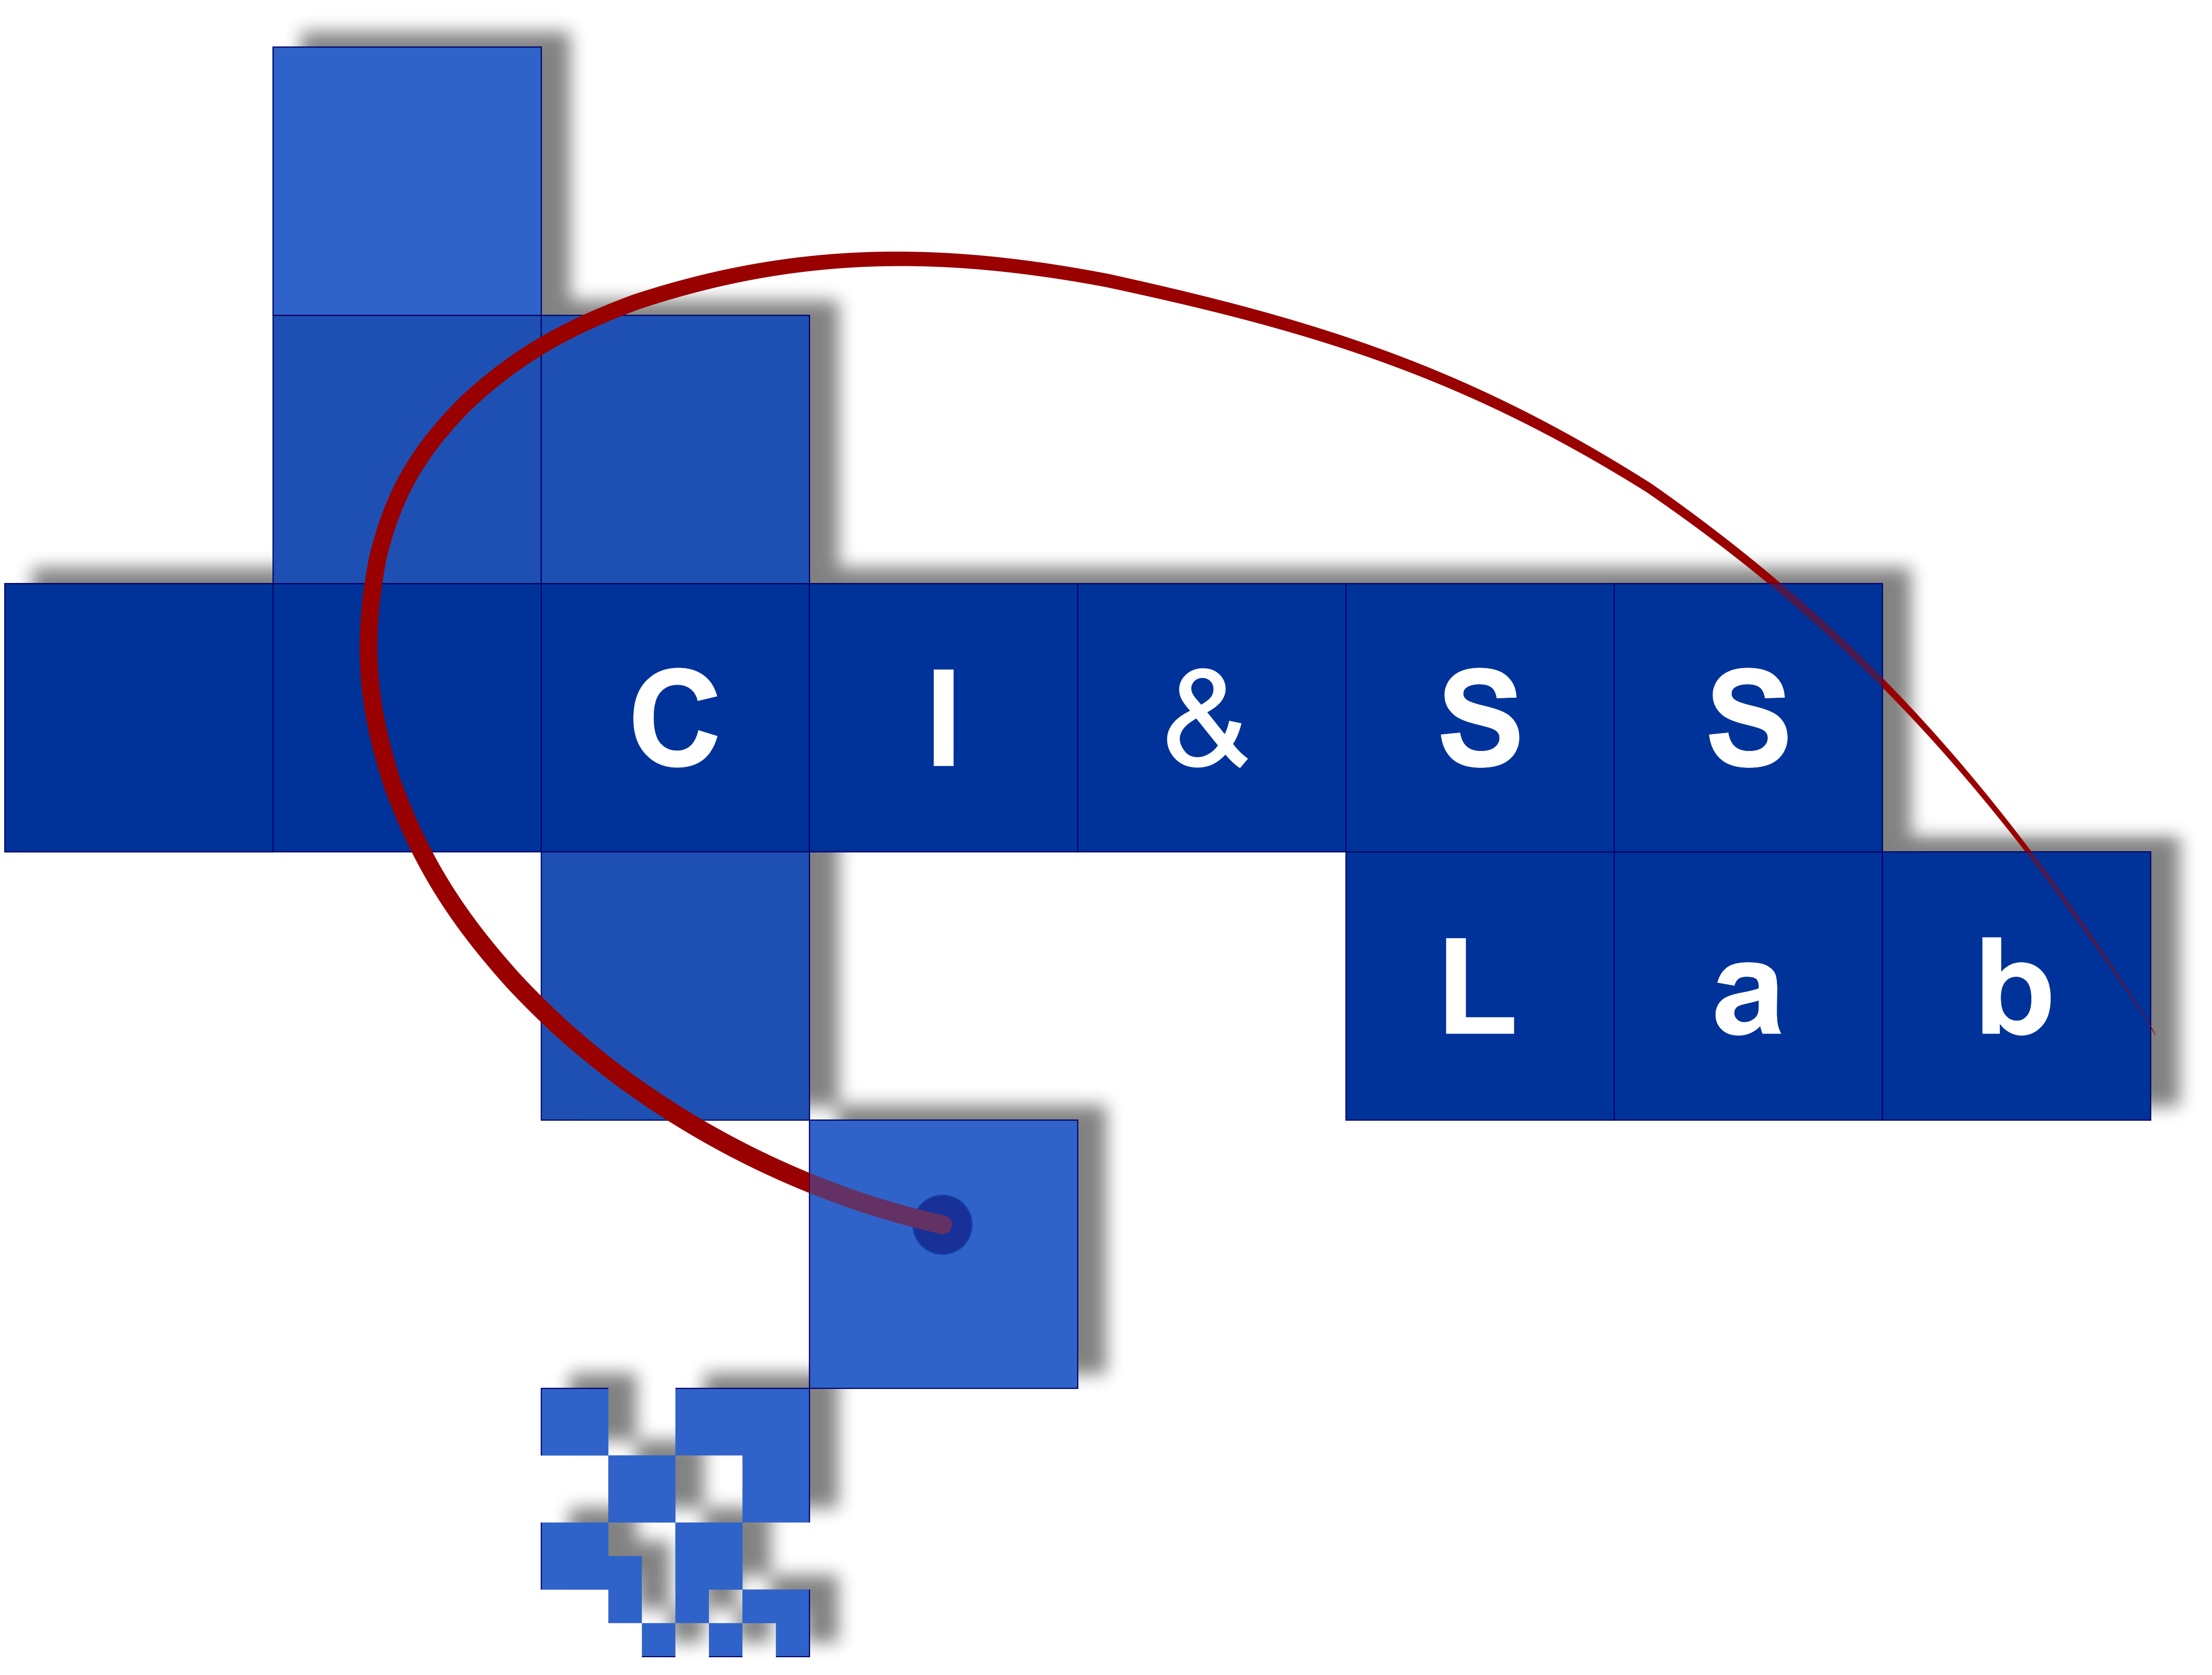
\includegraphics[width=0.32\textwidth]{assets/cisslab_logo.png}
\caption{CI\&SS Laboratory of the University of Naples ``Parthenope''.}
\label{fig:cisslab-logo}
\end{figure}

\subsection{Experiment Configurations}
\label{sec:experiment-configurations}

The pipeline was executed across multiple configurations, obtained by varying the following parameters:

\paragraph{Geographical scope.} Experiments were conducted on all five benchmark datasets described in Chapter~\ref{cap:data}: the New York metropolitan area (NY), Texas (TX), the U.S. Northeast, the U.S. South, and the set of all U.S. states except Alaska (ALL). Comparison is thereby enabled across socio-economically contrasting settings, ranging from a single metropolitan area to a national-scale dataset with over 1.4 million training instances.

\paragraph{Classifiers.} Two classifiers with fundamentally different decision boundary geometries were used: CatBoost, a gradient-boosted tree ensemble that produces axis-aligned decision splits, and MLP (Multi-Layer Perceptron), which produces smooth non-linear decision surfaces. As discussed in Chapter~\ref{cap:method}, the use of two structurally distinct classifiers allows verification that the patterns identified by the pipeline reflect properties of the data rather than artifacts of a particular model family. Since the adapted BoCSoR method is model-agnostic, patterns that emerge consistently across both classifiers carry stronger evidential weight.

\paragraph{Neighbourhood size $k$.} The number of counterfactual neighbours used in the BoCSoR analysis was varied across the set $k \in \{1, 3, 5, 7, 9, 11, 13, 15\}$. Small values of $k$ focus the analysis on the closest counterfactual neighbours, capturing the most local decision-boundary structure. Larger values broaden the neighbourhood, potentially revealing more stable and generalizable patterns at the cost of including more distant counterfactuals. By evaluating across the full range, the experiments assess the sensitivity of the extracted rules to the neighbourhood size and identify patterns that persist across multiple scales.

\paragraph{Boundary percentile $P$.} The percentile threshold for boundary instance selection was varied across $P \in \{10\%, 15\%, 20\%, 25\%\}$. This parameter controls how deep into the dataset the analysis reaches: at $P = 10\%$, only the $10\%$ of instances closest to the decision boundary are analyzed, yielding a focused but potentially sparse set of explanations. At $P = 25\%$, a broader population of near-boundary instances is included, increasing the volume of transactions available to the ARM stage but potentially diluting the signal with instances farther from the boundary. The variation of $P$ serves to assess the robustness of the extracted rules and to determine whether key patterns are stable across different boundary-proximity thresholds.

\paragraph{Overall configuration space.} The full experimental design spans 5 geographical scopes, 2 classifiers, 4 percentile values, and 8 neighbourhood sizes, yielding a total of $5 \times 2 \times 4 \times 8 = 320$ individual BoCSoR runs. Each run produces a separate transactional database, which is then independently processed by the macroscopic and microscopic ARM stages.

\subsection{Association Rule Mining Configuration}
\label{sec:arm-configuration}

The association rule mining stages operate on the transactional databases produced by BoCSoR and extract rules evaluated through three complementary metrics: support, confidence, and lift, as defined in Chapter~\ref{cap:method}.

To explore the space of possible threshold combinations systematically, the pipeline employs a grid search over support and confidence values. The support axis spans the range $[0.05, 1.00]$ and the confidence axis spans $[0.50, 1.00]$ for macroscopic rules, with step sizes automatically determined to produce approximately 40 levels per axis. For microscopic rules, the thresholds are set lower (support $\geq 0.01$, confidence $\geq 0.30$) to accommodate the smaller transaction sets that result from filtering to specific macroscopic rule anchors.

Rules whose lift falls within the interval $[0.75, 1.25]$ are discarded, as they represent near-independent co-occurrences that carry no meaningful associative information. Only rules with lift above $1.25$ (positive correlation) or below $0.75$ (negative correlation) are retained for analysis.

This grid-search approach avoids the need to commit to a single pair of thresholds \textit{a priori}. Instead, a complete landscape of rule counts is produced at each combination of support and confidence, making it possible to observe how the number of surviving rules varies as the quality bar is raised. Rules that persist at high support and high confidence thresholds are the strongest and most statistically reliable.

\subsection{Semantic Classification of Association Rules}
\label{sec:semantic-classification}

To interpret the extracted rules in the context of fairness and actionability, each rule is classified into one of three semantic categories based on the features it involves. This classification is applied to both macroscopic rules (which operate at the feature-name level, e.g., $\texttt{SCHL} \Rightarrow \texttt{OCCP}$) and microscopic rules (which operate at the feature-category level, e.g., $\texttt{SCHL=Bachelors} \Rightarrow \texttt{OCCP=Management}$).

\paragraph{Actionable rules.} A rule is classified as \emph{actionable} if \textbf{all} features appearing in both its antecedent and consequent belong exclusively to the set of actionable features: $\{\texttt{SCHL}, \texttt{COW}, \texttt{WKHP}, \texttt{OCCP}\}$. These features represent variables that a person can, at least in principle, modify through individual effort or choice: educational attainment, class of worker, weekly working hours, and occupation. Actionable rules capture the merit-based logic of the classifier, describing patterns such as ``higher education is associated with managerial occupations near the income boundary.''

\paragraph{Biased rules.} A rule is classified as \emph{biased} if it contains \textbf{at least one} sensitive feature: $\texttt{SEX}$ (sex) or $\texttt{RAC1P}$ (race). The rule may also contain any other features; the presence of even a single sensitive attribute is sufficient for classification as biased. Biased rules indicate that the classifier's decision logic, near the income boundary, is entangled with demographic attributes that should ideally be irrelevant to income prediction. A biased rule does not necessarily imply that the model is discriminatory in a legal or normative sense, but it signals that the boundary-crossing pattern involves a protected attribute and therefore warrants further scrutiny.

\paragraph{Other rules.} Rules that contain neither exclusively actionable features nor any sensitive feature are classified as \emph{other}. These typically involve contextual features such as age (\texttt{AGEP}), marital status (\texttt{MAR}), place of birth (\texttt{POBP}), or household relationship (\texttt{RELP}). While these rules contribute to the overall count and are used as the denominator for percentage calculations, they are not the primary focus of the analysis.

The classification is mutually exclusive: if a rule contains a sensitive feature, it is classified as biased regardless of whether it also contains actionable features. This conservative criterion reflects the principle that the presence of a protected attribute in the decision logic is always relevant from a fairness perspective.

At the same time, the interpretation adopted in this chapter remains deliberately descriptive and non-causal. The experimental analysis is limited to identifying, quantifying, and comparing statistical regularities in the extracted rules, namely recurring patterns of association among features near the classifier decision boundary. Consequently, terms such as \enquote{biased rules} must be understood as operational labels internal to the present analytical framework, not as definitive evidence of actual discrimination, nor as proof of an underlying sociological mechanism. Any stronger claim about real-world discriminatory phenomena, structural inequality, or the sociological meaning of the observed associations would require a separate domain-level assessment by qualified experts, such as sociologists or specialists in the application context. No such claims are made here, and no causal or normative conclusions are inferred beyond the empirical description of the patterns detected in the data and in the model behavior.

\section{Experimental Results}
\label{sec:main-results}

This section presents the main findings, organized from high-threshold baselines to detailed pattern analysis.

\subsection{High-Threshold Baseline}

At support $\geq 0.25$ and support $\geq 0.30$, no actionable or biased rules survive in any geographical scope, for either classifier, at any percentile or neighbourhood size. The only rules that persist at these thresholds involve contextual features such as age, marital status, and place of birth.

This negative result establishes the context for all subsequent findings: the merit-based and bias-related signals in the classifier's decision logic are statistically weaker than the contextual signals. They emerge only at lower support thresholds, meaning that a smaller, though still substantial, fraction of the boundary population is affected.

\subsection{Macroscopic Results at Support \texorpdfstring{$\geq 0.20$}{>= 0.20}}

At support $\geq 0.20$, the first biased rules appear. They emerge exclusively in Texas, and no actionable rules survive at this threshold in any state. Table~\ref{tab:macro-sup020} summarizes the findings.

\begin{table}[htbp]
\centering
\renewcommand{\arraystretch}{1.2}
\caption{Macroscopic rules at support $\geq 0.20$. Only configurations with at least one biased rule are shown.}
\label{tab:macro-sup020}
\begin{tabular}{>{\raggedright\arraybackslash}p{0.14\textwidth} >{\raggedright\arraybackslash}p{0.14\textwidth} p{0.08\textwidth} p{0.06\textwidth} p{0.12\textwidth} p{0.10\textwidth} p{0.10\textwidth}}
  \toprule
  \textbf{State} & \textbf{Classifier} & \textbf{Pct} & \textbf{$k$} & \textbf{Total} & \textbf{Action.} & \textbf{Biased} \\
  \midrule
  TX & CatBoost & 20 & 15 & 9 & 0 & 9 \\
  TX & MLP & 20 & 15 & 1 & 0 & 1 \\
  TX & CatBoost & 25 & 13 & 3 & 0 & 3 \\
  TX & CatBoost & 25 & 15 & 39 & 0 & 27 \\
  TX & MLP & 25 & 15 & 24 & 0 & 15 \\
  \bottomrule
\end{tabular}
\renewcommand{\arraystretch}{1.0}
\end{table}

All biased rules at this threshold share the same structural pattern: they involve race (\texttt{RAC1P}) and occupation (\texttt{OCCP}), often combined with education (\texttt{SCHL}) and age (\texttt{AGEP}). No biased rule at this threshold involves sex (\texttt{SEX}). All rules belong to class~0, i.e., they characterize the decision boundary toward lower income.

\subsection{Macroscopic Results at Support \texorpdfstring{$\geq 0.10$}{>= 0.10}}

At support $\geq 0.10$, both actionable and biased rules emerge across multiple geographical scopes, revealing a clear geographic asymmetry. Table~\ref{tab:macro-sup010} summarizes the distribution.

\begin{table}[htbp]
\centering
\renewcommand{\arraystretch}{1.2}
\caption{Macroscopic actionable and biased rules at support $\geq 0.10$, aggregated across all configurations.}
\label{tab:macro-sup010}
\begin{tabular}{>{\raggedright\arraybackslash}p{0.18\textwidth} p{0.14\textwidth} p{0.14\textwidth} p{0.38\textwidth}}
  \toprule
  \textbf{Scope} & \textbf{Actionable} & \textbf{Biased} & \textbf{Observation} \\
  \midrule
  NY & 123 & 52 & Actionable dominates ($2.4\times$) \\
  TX & 157 & 655 & Biased dominates ($4.2\times$) \\
  Northeast & 30 & 0 & Only actionable \\
  South & 28 & 102 & Biased dominates ($3.6\times$) \\
  ALL & 0 & 0 & No signal \\
  \bottomrule
\end{tabular}
\renewcommand{\arraystretch}{1.0}
\end{table}

\subsection{Macroscopic Results at Support \texorpdfstring{$\geq 0.05$}{>= 0.05}}

Lowering the support threshold to $0.05$ completes the picture. At this level, both actionable and biased rules appear in all five geographical scopes, including the national benchmark (ALL). Table~\ref{tab:macro-sup005} reports the full distribution.

\begin{table}[htbp]
\centering
\renewcommand{\arraystretch}{1.2}
\caption{Macroscopic actionable and biased rules at support $\geq 0.05$ and their ratio.}
\label{tab:macro-sup005}
\begin{tabular}{>{\raggedright\arraybackslash}p{0.18\textwidth} p{0.14\textwidth} p{0.14\textwidth} p{0.14\textwidth} p{0.24\textwidth}}
  \toprule
  \textbf{Scope} & \textbf{Actionable} & \textbf{Biased} & \textbf{Ratio} & \textbf{Observation} \\
  \midrule
  Northeast & 209 & 276 & $1.3\times$ & Nearly balanced \\
  ALL & 67 & 131 & $2.0\times$ & Mild bias prevalence \\
  NY & 303 & 796 & $2.6\times$ & Moderate bias \\
  TX & 287 & 2213 & $7.7\times$ & Strong bias \\
  South & 188 & 2213 & $11.8\times$ & Dominant bias \\
  \bottomrule
\end{tabular}
\renewcommand{\arraystretch}{1.0}
\end{table}

At this threshold, several additional findings emerge. The national benchmark (ALL) now produces 67 actionable and 131 biased rules, but these disappear already at support $\geq 0.07$, indicating that the national-level signal is real but extremely weak. The Northeast, which at support $\geq 0.10$ appeared entirely free of biased rules, now shows 276 biased rules at support $\geq 0.05$. However, these are statistically fragile: they drop to a single rule at support $\geq 0.07$ and vanish entirely at $\geq 0.10$. The Northeast may therefore be regarded as the cleanest benchmark, where any race-occupation entanglement is marginal.

The geographic asymmetry in the balance between actionable and biased rules is illustrated in Figure~\ref{fig:actionable-vs-biased}. The bias-to-actionable ratio increases monotonically from the Northeast ($1.3\times$) through the national aggregate ($2.0\times$), New York ($2.6\times$), and Texas ($7.7\times$) to the South ($11.8\times$), correlating with the socio-economic gradient described in Chapter~\ref{cap:data}.

\begin{figure}[htbp]
\centering
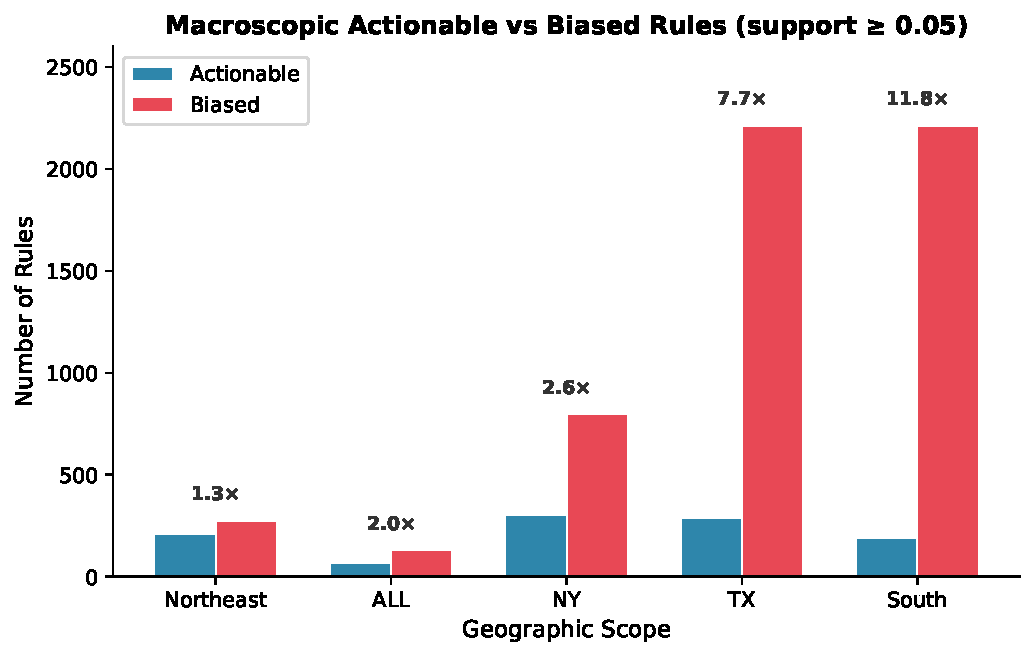
\includegraphics[width=0.85\textwidth]{assets/fig_actionable_vs_biased.pdf}
\caption{Macroscopic actionable and biased rule counts by geographic scope at support $\geq 0.05$. The bias-to-actionable ratio (annotated above each pair) increases from the more affluent benchmarks to those with higher poverty concentration.}
\label{fig:actionable-vs-biased}
\end{figure}

\subsection{Decay of Rules with Increasing Support}

Table~\ref{tab:decay} shows how actionable and biased rules disappear as the support threshold increases. This analysis reveals the relative statistical robustness of the two signals.

\begin{table}[htbp]
\centering
\renewcommand{\arraystretch}{1.2}
\caption{Actionable and biased rule counts at increasing support thresholds (summed across all configurations at the lowest confidence level).}
\label{tab:decay}
\resizebox{\textwidth}{!}{%
\begin{tabular}{>{\raggedright\arraybackslash}p{0.12\textwidth} *{5}{p{0.15\textwidth}}}
  \toprule
  \textbf{Support} & \textbf{ALL} & \textbf{NY} & \textbf{TX} & \textbf{Northeast} & \textbf{South} \\
  \midrule
  $\geq 0.05$ & 67 / 131 & 303 / 796 & 287 / 2213 & 209 / 276 & 187 / 2213 \\
  $\geq 0.07$ & 3 / 0 & 0 / 0 & 36 / 147 & 66 / 1 & 57 / 345 \\
  $\geq 0.10$ & 0 / 0 & 123 / 52 & 157 / 655 & 27 / 0 & 28 / 102 \\
  $\geq 0.15$ & 0 / 0 & 13 / 0 & 40 / 276 & 0 / 0 & 0 / 0 \\
  $\geq 0.20$ & 0 / 0 & 0 / 0 & 0 / 55 & 0 / 0 & 0 / 0 \\
  $\geq 0.25$ & 0 / 0 & 0 / 0 & 0 / 0 & 0 / 0 & 0 / 0 \\
  \bottomrule
\end{tabular}%
}
\renewcommand{\arraystretch}{1.0}
\begin{flushleft}
\small Each cell shows actionable / biased counts. NY values at support $\geq 0.07$ follow the same grid as other states.
\end{flushleft}
\end{table}

The decay patterns reveal two contrasting behaviors. In New York and the Northeast, actionable rules are more persistent than biased rules: they survive at higher support thresholds, indicating that the merit-based signal is statistically stronger than the bias signal. In Texas and the South, the opposite holds: biased rules survive up to support $\geq 0.20$ (Texas) or $\geq 0.10$ (South), while actionable rules disappear earlier. The race-occupation entanglement in these benchmarks is therefore statistically more robust than the merit-based decision patterns. Figure~\ref{fig:decay} visualizes this differential persistence.

\begin{figure}[htbp]
\centering
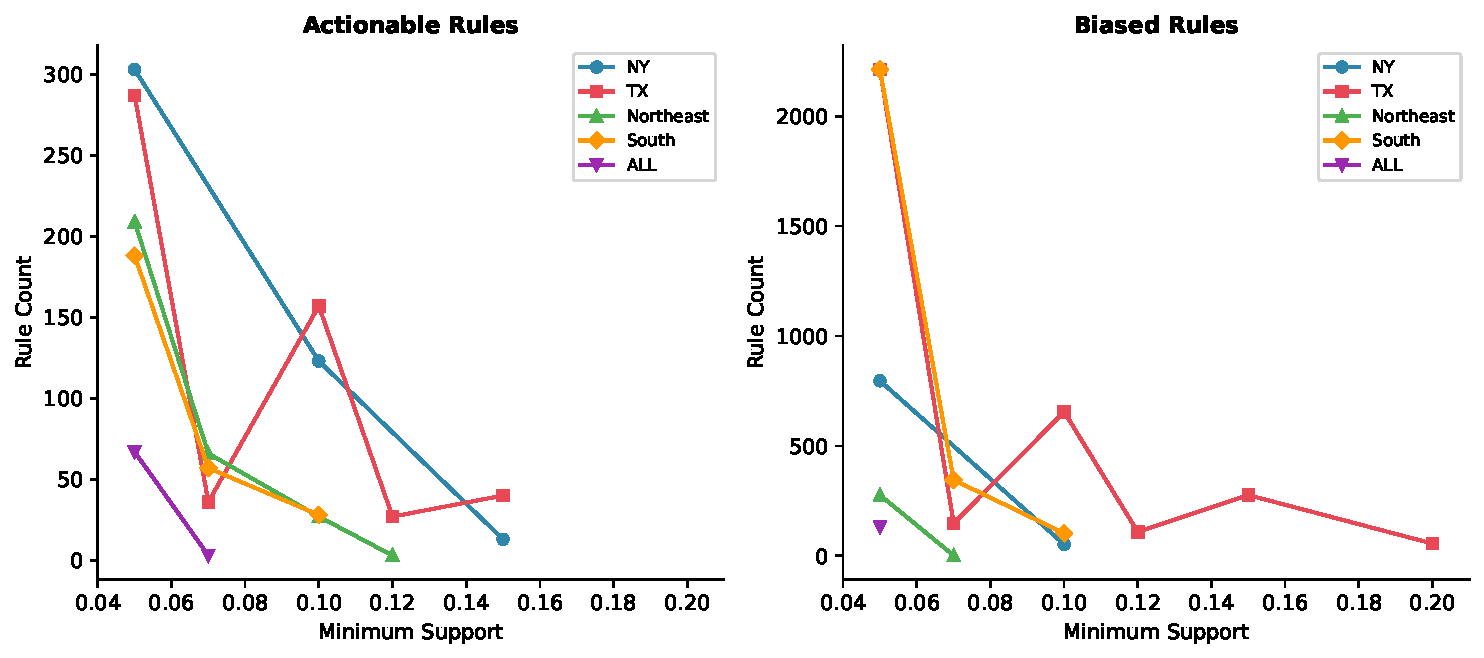
\includegraphics[width=\textwidth]{assets/fig_decay.pdf}
\caption{Decay of actionable (left) and biased (right) rules with increasing minimum support threshold. In New York and the Northeast, actionable rules persist at higher thresholds; in Texas and the South, biased rules are more robust. The ALL benchmark signal vanishes earliest.}
\label{fig:decay}
\end{figure}

\subsection{Class Asymmetry}

A consistent pattern emerges: the strong asymmetry between the two boundary directions.The vast majority of actionable and biased rules belong to class~0, which characterizes the boundary toward lower income (below the region-specific threshold $\theta$ defined in Chapter~\ref{cap:data}).

\begin{table}[htbp]
\centering
\renewcommand{\arraystretch}{1.2}
\caption{Actionable and biased rules by class direction (no support filter).}
\label{tab:class-asymmetry}
\begin{tabular}{>{\raggedright\arraybackslash}p{0.14\textwidth} p{0.18\textwidth} p{0.18\textwidth} p{0.36\textwidth}}
  \toprule
  \textbf{Class} & \textbf{Actionable} & \textbf{Biased} & \textbf{Note} \\
  \midrule
  Class 0 & 1018 & 5584 & All 5 scopes \\
  Class 1 & 36 & 45 & NY only (CatBoost and MLP) \\
  \bottomrule
\end{tabular}
\renewcommand{\arraystretch}{1.0}
\end{table}

Class~1 rules (boundary toward higher income, above $\theta$) are present only in New York, only at $k = 13$ and $k = 15$, and only at very low support ($0.05$--$0.06$). Despite their low support, these rules exhibit remarkably high lift values ($5.0$--$5.8$), indicating that the underlying patterns, while rare, are far from random. The same structural signatures observed for class~0 are also followed by class~1 rules: $\texttt{COW} \Rightarrow \texttt{OCCP}$ for actionable rules and $\texttt{RAC1P} \Rightarrow \texttt{OCCP}$ for biased rules.

This asymmetry suggests that the classifier's decision logic is more structured, and more susceptible to bias, when predicting who falls below the income threshold than when predicting who rises above it. The fact that the only exception occurs in New York, the most affluent and urbanized benchmark, is consistent with the hypothesis that class~1 patterns require a specific demographic structure to emerge.

\subsection{Dominant Macroscopic Patterns}

The actionable and biased rules that survive across multiple thresholds share distinct structural signatures. A deeper analysis of their composition reveals geographic variations in both the type of bias and the specific features involved.

\paragraph{Actionable pattern.} The dominant actionable pattern across all states is $\texttt{COW} \Rightarrow \texttt{OCCP}$ (class of worker predicts occupation), often combined with \texttt{SCHL} (education) and \texttt{WKHP} (working hours). This pattern appears in all five geographical scopes and accounts for the majority of actionable rules. The strongest individual actionable rule, observed in Texas at $k = 15$ and $P = 25\%$, achieves support $0.197$, confidence $0.857$, and lift $1.49$. In New York, the same pattern reaches higher lift values ($3.26$) but lower support ($0.174$).

\paragraph{Biased pattern: race and occupation.} The dominant biased pattern is $\texttt{RAC1P} \Rightarrow \texttt{OCCP}$ (race predicts occupation), often combined with \texttt{SCHL} and \texttt{AGEP}. This pattern appears in all five geographical scopes and is the strongest biased signal in every benchmark except the South. The strongest individual biased rule, observed in Texas, achieves support $0.236$, confidence $0.892$, and lift $1.55$. Rules involving race account for the vast majority of biased rules in every scope: $100\%$ in ALL, $77\%$ in NY, $79\%$ in TX, $67\%$ in the Northeast, and $91\%$ in the South.

\paragraph{Biased pattern: sex and occupation.} Contrary to what might be expected from the high-threshold analysis, sex (\texttt{SEX}) does appear in biased rules at support $\geq 0.05$. The pattern $\texttt{SEX} \Rightarrow \texttt{OCCP}$ emerges in four out of five scopes: NY ($186$ rules), TX ($467$), Northeast ($90$), and South ($190$). Only the ALL benchmark produces no sex-related biased rules. However, the sex signal is consistently weaker than the race signal: SEX rules have lower support (maximum $0.120$ in TX vs. $0.236$ for RAC1P) and lower lift. The Northeast shows the highest relative contribution of SEX, where $33\%$ of biased rules involve sex rather than race.

\paragraph{Geographic variation: the South and place of birth.} The South exhibits a unique biased pattern not observed as dominant in any other benchmark: $\texttt{RAC1P} \Rightarrow \texttt{POBP}$ (race predicts place of birth). This pattern accounts for $1{,}631$ out of $2{,}213$ biased rules in the South ($74\%$), making it the single most frequent biased association in that scope. By contrast, New York produces zero POBP-related biased rules, and in TX the figure is $327$ ($15\%$). This finding suggests that in the South, the classifier's decision boundary entangles race not primarily with occupation but with geographic origin, reflecting the distinct demographic structure of the region.

\paragraph{Independence of RAC1P and SEX.} The two sensitive features operate almost entirely independently in the extracted rules. Only $18$ rules out of $5{,}629$ biased rules ($0.3\%$) contain both \texttt{RAC1P} and \texttt{SEX}, and these appear exclusively in Texas. In all other scopes, no biased rule involves both sensitive attributes simultaneously. This indicates that race-related and sex-related bias, where present, follow separate structural paths in the classifier's decision logic.

The composition of biased rules by sensitive feature is illustrated in Figure~\ref{fig:bias-composition}.

\begin{figure}[htbp]
\centering
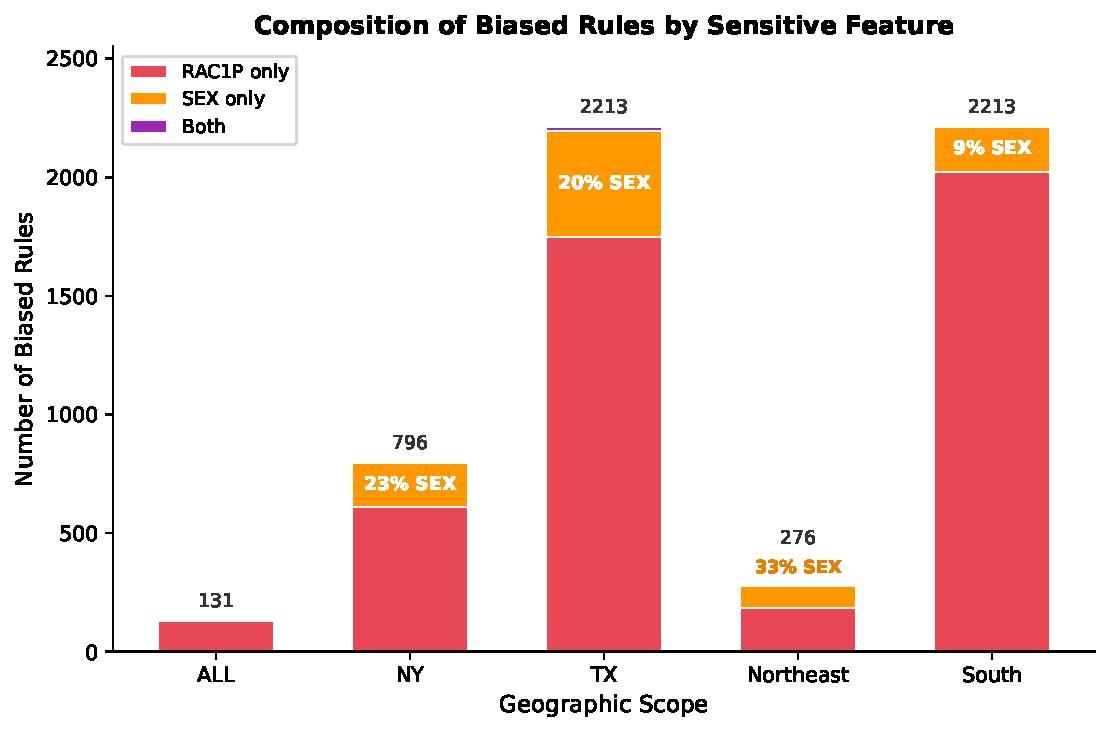
\includegraphics[width=0.85\textwidth]{assets/fig_bias_composition.pdf}
\caption{Composition of biased rules by sensitive feature across geographic scopes. Race (\texttt{RAC1P}) dominates in all benchmarks. Sex (\texttt{SEX}) contributes a secondary signal, most prominently in the Northeast ($33\%$) and New York ($23\%$). The two sensitive features almost never co-occur in the same rule.}
\label{fig:bias-composition}
\end{figure}

\subsection{Effect of Configuration Parameters}

\paragraph{Classifier comparison.} The same structural patterns are identified by both CatBoost and MLP, confirming the model-agnostic property of the pipeline. CatBoost produces more biased rules than MLP, particularly in Texas ($1150$ vs. $1063$ at support $\geq 0.05$). This is consistent with the nature of gradient-boosted trees, whose axis-aligned splits capture interactions between categorical features more readily than the smooth decision surfaces of MLP.

\paragraph{Neighbourhood size and percentile.} Larger values of $k$ (13 and 15) and higher percentiles ($20\%$ and $25\%$) produce more rules. The most informative configurations for surfacing both actionable and biased rules are $k = 15$ with $P = 25\%$. Class~1 rules appear only at $k = 13$ and $k = 15$, indicating that the higher-income boundary patterns require broader counterfactual neighbourhoods to be detected.

\paragraph{Decay with increasing support.} The differential persistence of actionable and biased rules at increasing support thresholds varies by geographic scope. In New York and the Northeast, actionable rules are more persistent; in Texas and the South, biased rules dominate. This asymmetry constitutes one of the main empirical findings documented in the thesis.

\subsection{Microscopic Results}
\label{sec:micro-results}

The macroscopic analysis identifies which features co-occur at the decision boundary; the microscopic analysis reveals the specific category values that materialize those structural dependencies. For each macroscopic rule that survives the support $\geq 0.10$ threshold, the pipeline extracts value-level rules from the filtered transaction subsets. After applying microscopic thresholds (support $\geq 0.03$, confidence $\geq 0.70$, lift $\geq 2.0$), the analysis yields $30{,}252$ actionable and $31{,}353$ biased microscopic rules. Texas dominates both categories, contributing over $99\%$ of the micro rules due to its larger volume of surviving macroscopic mothers.

\subsubsection{Microscopic Actionable Patterns}

The dominant micro-level actionable pattern across all scopes is the association between public-sector employment and the education sector. In Texas, the strongest rule is
\begin{center}
\texttt{COW=Local-Government-Employee} $\Rightarrow$ \texttt{OCCP=Educational-Instruction-And-Library}
\end{center}
with support $0.271$, confidence $0.772$, and lift $2.34$. This means that among boundary instances where class of worker and occupation are jointly relevant for the prediction, $27\%$ involve public employees in education, and $77\%$ of those who are local government employees work in educational occupations. When combined with \texttt{SCHL=Bachelors-Degree}, the confidence rises to $0.888$ and the lift to $2.89$: a bachelor's degree essentially determines the specific occupation within the public sector near the income boundary.

In New York, a different actionable profile emerges: \texttt{COW=Employee-Private-Non-Profit} $\wedge$ \texttt{OCCP=Educational-Instruction-And-Library} $\Rightarrow$ \texttt{SCHL=Masters-Degree} (confidence $0.729$, lift $5.30$). The merit-based signal in New York therefore points to private non-profit education requiring a master's degree, whereas in Texas it points to public education requiring a bachelor's.

In the South, the same structural pattern materializes: \texttt{COW=Local-Government-Employee} $\wedge$ \texttt{SCHL=Bachelors-Degree} $\Rightarrow$ \texttt{OCCP=Educational-Instruction-And-Library} (support $0.052$, lift $3.65$).

\subsubsection{Microscopic Biased Patterns}

The microscopic biased rules reveal the specific demographic profiles entangled with the classifier's decision logic.

\paragraph{Texas: gendered education sector.} Sex is the dominant sensitive feature in Texas microscopic biased rules: \texttt{SEX=Female} appears in $12{,}621$ out of $30{,}729$ biased rules ($41\%$), while \texttt{SEX=Male} appears in only $3$. The strongest gendered pattern is
\begin{center}
\texttt{COW=Local-Government-Employee} $\wedge$ \texttt{SEX=Female} $\Rightarrow$ \texttt{OCCP=Educational-Instruction-And-Library}
\end{center}
with support $0.114$ and confidence $0.787$. This reveals that the same occupation-employer pattern that drives actionable rules becomes biased when it is inseparable from the sex of the worker. In parallel, race enters through a different occupational channel: \texttt{OCCP=Office-And-Administrative-Support} $\wedge$ \texttt{SEX=Female} $\Rightarrow$ \texttt{RAC1P=Two-Or-More-Races} (support $0.073$, confidence $0.820$), and the construction sector is associated with \texttt{RAC1P=White-Alone} ($3{,}385$ rules).

\paragraph{New York: white women in office work.} In New York, the micro biased rules describe a specific demographic profile: white women (\texttt{RAC1P=White-Alone}, \texttt{SEX=Female}) in office-administrative occupations living as dependents in the household (\texttt{RELP=Biological-Son-Or-Daughter}). The highest-lift rule,
\begin{center}
\texttt{RAC1P=White-Alone} $\wedge$ \texttt{SEX=Female} $\wedge$ \texttt{WKHP=Full-Time} $\Rightarrow$ \texttt{OCCP=Office-And-Administrative} $\wedge$ \texttt{RELP=Biological-Son-Or-Daughter}
\end{center}
achieves lift $7.64$, indicating a pattern $7.6$ times more likely than expected under independence. Both sensitive features (race and sex) co-occur in $93$ out of $590$ micro biased rules, a substantially higher rate of co-occurrence than at the macroscopic level.

\paragraph{South: geographic origin and race.} Only one microscopic biased pattern survives the quality thresholds in the South:
\begin{center}
\texttt{POBP=Georgia} $\Rightarrow$ \texttt{RAC1P=Black-Or-African-American-Alone}
\end{center}
with support $0.035$, confidence $0.719$, and lift $2.27$. This is the concrete materialization of the macroscopic pattern $\texttt{RAC1P} \Rightarrow \texttt{POBP}$ that distinguishes the South from all other benchmarks: at the income boundary, being born in Georgia is strongly associated with being Black. The fact that this is the sole surviving micro biased rule in the South underscores the specificity of the regional bias signal.

\subsubsection{Summary of Microscopic Findings}

Table~\ref{tab:micro-summary} summarizes the dominant microscopic patterns by geographic scope and rule type.

\begin{table}[htbp]
\centering
\renewcommand{\arraystretch}{1.2}
\caption{Dominant microscopic patterns by scope and type. Support and lift refer to the strongest instance of each pattern.}
\label{tab:micro-summary}
\begin{tabularx}{\textwidth}{>{\raggedright\arraybackslash}p{0.10\textwidth} >{\raggedright\arraybackslash}p{0.10\textwidth} >{\raggedright\arraybackslash}X >{\centering\arraybackslash}p{0.09\textwidth} >{\centering\arraybackslash}p{0.09\textwidth} >{\centering\arraybackslash}p{0.09\textwidth}}
  \toprule
  \textbf{Scope} & \textbf{Type} & \textbf{Pattern} & \textbf{Supp.} & \textbf{Conf.} & \textbf{Lift} \\
  \midrule
  TX & Action. & Local-Govt-Employee $\Rightarrow$ Educational-Instruction & 0.271 & 0.772 & 2.34 \\
  TX & Biased & Local-Govt-Employee $\wedge$ Female $\Rightarrow$ Educational-Instruction & 0.114 & 0.787 & 3.19 \\
  TX & Biased & Office-Admin $\wedge$ Female $\Rightarrow$ Two-Or-More-Races & 0.073 & 0.820 & 2.08 \\
  NY & Action. & Non-Profit $\wedge$ Educational-Instruction $\Rightarrow$ Masters-Degree & 0.036 & 0.729 & 5.30 \\
  NY & Biased & White-Alone $\wedge$ Female $\wedge$ Full-Time $\Rightarrow$ Office-Admin $\wedge$ Biological-Child & 0.036 & 0.703 & 7.64 \\
  South & Action. & Local-Govt $\wedge$ Bachelors $\Rightarrow$ Educational-Instruction & 0.052 & 0.712 & 3.65 \\
  South & Biased & Born-Georgia $\Rightarrow$ Black-Or-African-American & 0.035 & 0.719 & 2.27 \\
  \bottomrule
\end{tabularx}
\renewcommand{\arraystretch}{1.0}
\end{table}

The microscopic analysis confirms and enriches the macroscopic findings. The structural dependency $\texttt{COW} \Rightarrow \texttt{OCCP}$ materializes as a public-education pattern in every scope where it appears. The structural dependency $\texttt{RAC1P} \Rightarrow \texttt{OCCP}$ reveals that the entanglement is not uniform across races or occupations: in Texas it involves the education sector and female workers, in New York it involves white women in office work, and in the South it takes the form of a geographic-racial association specific to the state of Georgia. These findings demonstrate that the hierarchical macro-to-micro analysis provides explanatory depth that would be inaccessible from either level alone.

\chapter{Conclusions and Future Work}
\label{cap:conclusions}
% !TEX root = ../main.tex

\section{Conclusions}
\label{sec:conclusions-summary}

This work proposed and evaluated a pipeline for extracting global, human-interpretable explanations of tabular classifiers through the combination of boundary-based counterfactual feature importance and hierarchical Association Rule Mining. The pipeline was applied to five geographical benchmarks derived from the 2024 American Community Survey, with two structurally different classifiers and a systematic grid search over support and confidence thresholds.

The empirical evaluation produced several findings that, taken together, support the usefulness of the proposed approach. At the macroscopic level, the pipeline surfaced a consistent structural vocabulary: $\texttt{COW} \Rightarrow \texttt{OCCP}$ for actionable rules and $\texttt{RAC1P} \Rightarrow \texttt{OCCP}$ for biased rules, both present in all five scopes. At the same time, the ratio between actionable and biased rules varied systematically with the socio-economic profile of the benchmark, ranging from $1.3\times$ in the Northeast to $11.8\times$ in the South at support $\geq 0.05$. This geographic asymmetry is one of the most robust signals documented in this work: it persists across thresholds, classifiers, and parameter settings.

The decay analysis refined this picture. Actionable rules are statistically more robust than biased rules in New York and the Northeast, where they survive at higher support thresholds; biased rules are more robust in Texas and the South, where they persist up to support $\geq 0.20$ and $\geq 0.10$ respectively. The national benchmark (ALL) exhibits the weakest signal, confirming that aggregating heterogeneous populations dilutes locally identifiable patterns.

The microscopic analysis provided the semantic depth that macroscopic patterns cannot supply on their own. In Texas, the dominant actionable pattern materializes as public-sector employment in educational occupations (\texttt{COW=Local-Government-Employee} $\Rightarrow$ \texttt{OCCP=Educational-Instruction-And-Library}, support $0.271$); the dominant biased pattern combines the same occupational signature with \texttt{SEX=Female}, producing the profile of the female public-school teacher. In New York, biased rules describe white women in office work living as biological daughters, with lift values up to $7.64$. In the South, only one microscopic biased rule survives the quality filters, $\texttt{POBP=Georgia} \Rightarrow \texttt{RAC1P=Black-Or-African-American-Alone}$, which is the concrete expression of the unique macroscopic pattern $\texttt{RAC1P} \Rightarrow \texttt{POBP}$ distinctive to that benchmark.

A further finding concerns the asymmetry between the two classes. Actionable and biased rules dominate the boundary toward lower income (class~0) in all scopes. Rules on the boundary toward higher income (class~1) are observed only in New York, only at $k \in \{13, 15\}$, and at low support (around $0.05$), but they reach very high lift values ($5.0$ to $5.8$), indicating rare but strongly non-random patterns in the only benchmark where the upper-income regime produces detectable structure.

Overall, the pipeline operationalizes a principled separation between merit-based and demographically-entangled decision patterns, without committing to a single fairness metric and without making causal claims. The hierarchical design proved essential: macroscopic rules identified the structural skeleton, and microscopic rules revealed the specific demographic profiles animating it. Neither level alone would have been sufficient.

\section{Limitations}
\label{sec:conclusions-limitations}

The approach has limitations that should be made explicit.

\paragraph{Descriptive, not causal.} The analysis is purely associational. The labels ``actionable'' and ``biased'' are operational categories defined with respect to feature content, not claims about the causal structure of the classifier or about actual discrimination. Verifying that a biased rule corresponds to a causally discriminatory mechanism would require domain-level assessment by qualified experts and a causal-inference framework outside the scope of the thesis.

\paragraph{Boundary-focused.} The pipeline analyzes only instances close to the decision boundary, selected via a percentile threshold on counterfactual distance. This restriction is methodologically motivated (the boundary is where the classifier exhibits the highest uncertainty and therefore the most informative behavior) but implies that patterns confined to the interior of the class regions are not captured. Instances well inside the class-0 or class-1 region do not contribute to the extracted rules.

\paragraph{Dataset and domain specificity.} The experimental evaluation is limited to the 2024 ACS Income task and to five U.S.\ geographical benchmarks. Other Folktables tasks (public coverage, mobility, employment), other census years, other countries, and other socio-demographic domains have not been tested. The specific patterns documented here (e.g., the $\texttt{RAC1P} \Rightarrow \texttt{POBP}$ pattern in the South) are therefore context-dependent and should not be extrapolated without re-validation.

\paragraph{Classifier families.} The validation relies on two classifier families (CatBoost and MLP). Transformer-based tabular models (for example TabTransformer, FT-Transformer) and other architectures with substantially different inductive biases have not been examined. Although the pipeline is model-agnostic by construction, its behavior on such architectures remains an empirical question.

\paragraph{Information loss from categorization.} Continuous features (age, working hours) are discretized prior to the rule mining stages. This simplifies the combinatorial structure of the transaction database but loses fine-grained information. A finer bin structure, or a direct handling of mixed-type features in the rule mining itself, could in principle surface patterns that the current categorization obscures.

\paragraph{Threshold sensitivity.} The number of surviving rules depends strongly on the support, confidence, and lift thresholds chosen for filtering. The grid search mitigates this dependency by providing a landscape view, but it does not remove it. Reporting patterns that persist across multiple threshold combinations is a partial remedy; a fully threshold-free characterization of rule stability remains open.

\section{Future Work}
\label{sec:conclusions-future}

Several directions extend the work presented here.

\paragraph{Cross-task and cross-country replication.} A natural next step is to apply the pipeline to the other Folktables tasks (\texttt{ACSPublicCoverage}, \texttt{ACSMobility}, \texttt{ACSEmployment}, \texttt{ACSTravelTime}) and to census systems outside the United States where comparable microdata are available. Such replication would test the generality of the geographic asymmetry documented here and establish whether the $\texttt{RAC1P} \Rightarrow \texttt{POBP}$ pattern is specific to the U.S.\ South or emerges in analogous socio-economic settings elsewhere.

\paragraph{Temporal analysis.} Running the pipeline across multiple ACS release years would make it possible to track the evolution of actionable and biased patterns over time, detecting drift in the classifier's decision logic as the underlying population evolves. This is particularly relevant for fairness monitoring in production systems, where retraining introduces new boundary patterns that may differ from those validated at deployment.

\paragraph{Integration with causal inference.} The descriptive rules produced by the pipeline can serve as hypotheses for subsequent causal analysis. Methods such as do-calculus on the feature graph or interventional feature attribution could be applied to the variable interactions surfaced by the biased rules, converting associational findings into causal claims where the data-generating process is sufficiently well understood.

\paragraph{Bias-mitigation strategies guided by the extracted rules.} Once a set of biased rules has been identified, it can serve as a targeted intervention map. Rather than applying a global fairness constraint, one could remove or reweight the specific transaction sub-populations that instantiate the biased rules and retrain the classifier, assessing whether the pipeline no longer surfaces those rules in the retrained model. This would close the loop between explanation and mitigation.

\paragraph{Transformer-based tabular models.} Applying the pipeline to TabTransformer, FT-Transformer, SAINT, or similar architectures would test whether the structural patterns documented here (in particular $\texttt{COW} \Rightarrow \texttt{OCCP}$ and $\texttt{RAC1P} \Rightarrow \texttt{OCCP}$) are properties of the data or artifacts of the specific inductive biases of CatBoost and MLP.

\paragraph{Integration with formal fairness metrics.} The semantic classification of rules is deliberately independent of traditional fairness metrics (demographic parity, equalized odds, predictive parity). Connecting the two perspectives, for example by computing the contribution of each biased rule to a given disparity measure, would provide a quantitative bridge between rule-based and metric-based fairness analysis.

\paragraph{Threshold-free pattern characterization.} An appealing extension is to replace the current support--confidence grid search with a threshold-free ranking of rule stability, for instance by aggregating persistence across the full parameter landscape. This would eliminate the residual dependence on threshold choices and provide a single scalar measure of confidence per rule.

Taken together, these directions suggest that the proposed pipeline is best viewed not as a final artifact but as a reusable methodology: a way of organizing the interpretation of tabular classifiers that can be instantiated in many domains, time periods, and model families, and that produces outputs amenable to both qualitative inspection and quantitative downstream analysis.

\clearpage
\nocite{*}
\printbibliography[
  title={References},
  nottype=online,
  heading=bibintoc
]

\printbibliography[
  title={Web References},
  type=online,
  heading=bibintoc
]

\newpage
\appendix
\titleformat{\chapter}[display]
  {\bfseries\fontsize{16pt}{18pt}\selectfont}
  {}
  {0pt}
  {}
% !TEX root = ../main.tex

\chapter{Pipeline Implementation Details}
\label{app:pipeline-implementation}

\section{Parallelization Strategy}
\label{app:parallelization}

Pipeline scalability is essential, since the national dataset includes over $1.4$ million training instances.
The adopted parallelization strategy uses Python's standard-library module \texttt{concurrent.\allowbreak futures}, combining process pools and thread pools depending on workload type.

\paragraph{Global Interpreter Lock and motivation of the concurrency choice.}
CPython is subject to the Global Interpreter Lock (GIL), which prevents simultaneous execution of Python bytecode by multiple threads in the same process.
For purely \texttt{CPU-bound} operations (e.g., independent processing of different years), independent processes are used (\texttt{ProcessPoolExecutor}), each with its own GIL.
For \texttt{I/O-bound} operations (census-data download, disk writing), threads are used (\texttt{ThreadPoolExecutor}), since system calls release the GIL while waiting.
For numerically intensive stage-2 operations (distance computation, model predictions), \texttt{ThreadPoolExecutor} is also used despite CPU-bound behavior, because underlying libraries (SciPy \texttt{cdist}, CatBoost, scikit-learn) are implemented in C/Cython and release the GIL during native computation, enabling true concurrency among threads.
This choice also avoids using \texttt{fork()} with BLAS libraries such as Apple Accelerate, whose internal state may not survive process duplication, causing non-deterministic deadlocks on macOS.

\paragraph{Memory sharing among workers.}
Where \texttt{ProcessPool\allowbreak Executor} is used (stage~1 multi-year), child processes are created with \texttt{spawn}: the child process is initialized from scratch, re-importing required modules without inheriting parent-process state.
This is the default behavior on macOS and Windows and is explicitly enforced by the pipeline for safety with BLAS libraries, as shown in Listing~\ref{lst:spawn-method}.

\begin{lstlisting}[style=pipeline,caption={Explicit \texttt{spawn} start method enforcement (\texttt{src/main.py}).},label={lst:spawn-method}]
def main() -> None:
    multiprocessing.set_start_method("spawn", force=True)
    parser = build_parser()
    args   = parser.parse_args()
\end{lstlisting}

In stage~2 and stage~4, where sharing concerns large objects and intensive numerical kernels, \texttt{ThreadPoolExecutor} is preferred: threads directly share parent-process heap memory without duplication, serialization, or process-start overhead, and avoid macOS deadlocks potentially induced by forking BLAS/Accelerate internal mutex state.

The number of workers is auto-detected at startup (Listing~\ref{lst:workers}), reserving 2 logical CPUs for the OS and the main process, and capping at 14 to prevent competing internal thread pools (CatBoost, SciPy) from degrading throughput.

\begin{lstlisting}[style=pipeline,caption={Worker count auto-detection (\texttt{src/main.py}).},label={lst:workers}]
# Formula: max(1, min(14, cpu_count - 2)).
# Reserves 2 logical CPUs for the OS and the main process; caps at 14
# to avoid competing CatBoost thread pools degrading throughput.
_DEFAULT_WORKERS = max(1, min(14, (os.cpu_count() or 4) - 2))
\end{lstlisting}

\paragraph{Stage~1 --- Download and preprocessing.}\fussy
Microdata download for each state is executed in parallel via \texttt{ThreadPoolExecutor} (up to 16 threads), leveraging GIL release during network calls.
Listing~\ref{lst:download-parallel} shows the parallel download implementation.

\begin{lstlisting}[style=pipeline,caption={Parallel per-state download via \texttt{ThreadPoolExecutor} (\texttt{src/create\_dataset.py}).},label={lst:download-parallel}]
n_workers = min(_IO_WORKERS, len(states))   # _IO_WORKERS = min(16, cpu_count)

with ThreadPoolExecutor(max_workers=n_workers) as executor:
    future_to_state = {
        executor.submit(
            _download_one_state,
            state, survey_year, horizon, survey, raw_dir,
        ): state
        for state in states
    }
    for future in as_completed(future_to_state):
        state = future_to_state[future]
        try:
            frames[state] = future.result()
        except Exception as exc:
            failures.append(state)

# Concatenate in the original order for reproducibility.
df = pd.concat([frames[s] for s in states if s in frames], ignore_index=True)
\end{lstlisting}

Column categorization uses vectorized NumPy and pandas operations (e.g., \texttt{np.searchsorted}, type casting, and column-wise mapping) that release the GIL in the dominant native kernels, and is parallelized through \texttt{ThreadPoolExecutor} (up to 8 threads).
Each column transform is independent and dispatched as a separate task (Listing~\ref{lst:categorize-parallel}).

\begin{lstlisting}[style=pipeline,caption={Parallel column categorization (\texttt{src/create\_dataset.py}).},label={lst:categorize-parallel}]
def categorize(df: pd.DataFrame) -> pd.DataFrame:
    transforms = [
        (col, fn) for col, fn in _build_column_transforms()
        if col in df.columns
    ]
    results: dict[str, pd.Series] = {}

    def _apply(col, fn, series):
        return col, fn(series)

    with ThreadPoolExecutor(
        max_workers=min(_CAT_WORKERS, len(transforms))  # _CAT_WORKERS = min(8, cpu_count)
    ) as executor:
        futures = {
            executor.submit(_apply, col, fn, df[col].copy()): col
            for col, fn in transforms
        }
        for future in as_completed(futures):
            col, result = future.result()
            results[col] = result

    # Reassemble in the original column order.
    out = df.copy()
    for col in df.columns:
        if col in results:
            out[col] = results[col]
    return out
\end{lstlisting}

The three output CSV files (dataset, train, test) are written concurrently with a 3-thread pool.
In multi-year runs, creation of each yearly dataset is delegated to an independent process via \texttt{ProcessPoolExecutor} (Listing~\ref{lst:multi-year}).

\begin{lstlisting}[style=pipeline,caption={Multi-year parallel execution via \texttt{ProcessPoolExecutor} (\texttt{src/main.py}).},label={lst:multi-year}]
# Multiple years: one process per year (CPU-bound + independent I/O).
workers = min(args.workers, len(args.years))

with ProcessPoolExecutor(max_workers=workers) as executor:
    future_to_year = {
        executor.submit(_process_year, year=y, **common_kwargs): y
        for y in args.years
    }
    for future in as_completed(future_to_year):
        y = future_to_year[future]
        try:
            _, n_train, n_test = future.result()
            completed[y] = (n_train, n_test)
        except Exception as exc:
            failed.append(y)
\end{lstlisting}

\paragraph{Stage~2 --- BoCSoR.}
This is the most computationally expensive stage.
The equivalent global Manhattan formulation introduced in Chapter~\ref{cap:method}
is advantageous here because it makes it possible to compute distances on the
full encoded representation in a single, uniform way. This simplifies the
execution flow and supports the optimization strategies adopted in the
pipeline.
Main optimizations are:

\begin{itemize}
  \item \textbf{Brute-force nearest-neighbor index}: scikit-learn's nearest-neighbor implementation is used with \texttt{algorithm=\textquotesingle brute\textquotesingle} and Manhattan metric.
  At 147 encoded dimensions, this is faster than tree-based methods (BallTree, KDTree), which degrade due to the curse of dimensionality.
  Two distinct indices are built (Listing~\ref{lst:nn-indices}): one with \texttt{n\_jobs=-1} for the initial boundary selection (multi-core via joblib, safe because the loky backend uses spawn-like semantics), and one with \texttt{n\_jobs=1} shared across \texttt{ThreadPoolExecutor} workers for the $k$-NN queries (avoids oversubscription from nested thread pools).

\begin{lstlisting}[style=pipeline,caption={Two NN index configurations for boundary selection and worker queries (\texttt{src/feature\_importance.py}).},label={lst:nn-indices}]
# Boundary selection: multi-core via joblib (loky backend, spawn-safe).
cf_nn_boundary = NearestNeighbors(
    algorithm="brute", metric="manhattan", n_jobs=-1,
)
cf_nn_boundary.fit(X_enc_cf.astype(np.float32))
min_dists, _ = cf_nn_boundary.kneighbors(X_orig_q, n_neighbors=1)
del cf_nn_boundary   # free memory -- no longer needed

# Worker NN index: n_jobs=1 (shared by ThreadPoolExecutor workers).
# Each thread calls kneighbors() concurrently; SciPy cdist (Cython)
# releases the GIL, enabling true thread-level parallelism.
def build_nn_index(X_enc):
    nn = NearestNeighbors(
        algorithm="brute",
        metric="manhattan",
        n_jobs=1,
    )
    nn.fit(X_enc.astype(np.float32))
    return nn
\end{lstlisting}

  \item \textbf{Single encoding pass}: the hybrid-encoded matrix (\textasciitilde560~MB in \texttt{float32} for the national dataset) is built once before the loop over $k$ values and reused for all $k$.
  Listing~\ref{lst:encode-hybrid} shows the pre-allocated encoding strategy.

\begin{lstlisting}[style=pipeline,caption={Pre-allocated hybrid encoding (\texttt{src/feature\_importance.py}).},label={lst:encode-hybrid}]
def encode_hybrid(df, rank_maps, nominal_maps, feature_cols):
    n = len(df)
    total_cols = n_encoded_cols(feature_cols, rank_maps, nominal_maps)
    # Pre-allocate: one contiguous block instead of many small arrays.
    out = np.empty((n, total_cols), dtype=np.float32)
    col_ptr = 0

    for col in feature_cols:
        if col in rank_maps:
            # Ordinal: rank -> min-max normalised to [0, 1]
            rmap     = rank_maps[col]
            max_rank = max(rmap.values())
            denom    = float(max_rank - 1) if max_rank > 1 else 1.0
            norm_map = {cat: (rank - 1) / denom for cat, rank in rmap.items()}
            out[:, col_ptr] = (
                df[col].map(norm_map).fillna(0.5)
                .to_numpy(dtype=np.float32)
            )
            col_ptr += 1
        else:
            # Nominal: one-hot / 2 -> each bit in {0.0, 0.5}
            cats = nominal_maps.get(col, [])
            col_vals = df[col].to_numpy()
            for cat in cats:
                out[:, col_ptr] = (col_vals == cat).astype(np.float32) * 0.5
                col_ptr += 1
    return out
\end{lstlisting}

  \item \textbf{Precomputed $k$-NN query}: the brute-force $k$-NN query is executed once with $k_{\text{query}}$ sized for the maximum $k$ value.
  Because the top-$k_1$ neighbours are always a prefix of the top-$k_2$ results ($k_1 < k_2$), a single query suffices for all $k$ values.
  Each per-$k$ run slices the first $k$ valid neighbours from the same precomputed arrays, eliminating $|\mathcal{K}|-1$ redundant $O(N \times M)$ distance computations (Listing~\ref{lst:nn-precompute}).

\begin{lstlisting}[style=pipeline,caption={Single $k$-NN precomputation reused across all $k$ values (\texttt{src/feature\_importance.py}).},label={lst:nn-precompute}]
max_k = max(k_values)
k_query_global = min(max(max_k * 50, 200), n_cf)

shared_nn: list[tuple[np.ndarray, np.ndarray]] = []
for chunk in shared_chunks:
    chunk_q = X_enc[chunk].astype(np.float32)
    dists_c, tops_c = cf_nn.kneighbors(chunk_q, n_neighbors=k_query_global)
    shared_nn.append((dists_c, tops_c))
# Reused across all k values -- no redundant O(N*M) computations.
\end{lstlisting}

  \item \textbf{Batch prediction}: for each boundary instance, all modified instances (one per counterfactual-feature pair, across all $k$ counterfactuals) are concatenated into a single pre-allocated NumPy array and passed to \texttt{model.predict()} in one call (Listing~\ref{lst:batch-predict}), eliminating per-feature Python round-trip overhead.

\begin{lstlisting}[style=pipeline,caption={Batched relevance check --- Algorithm~2 of BoCSoR (\texttt{src/feature\_importance.py}).},label={lst:batch-predict}]
# Build one modified instance per (counterfactual, differing_feature) pair.
batch_meta: list[tuple[int, int]] = []    # (cf_idx, feature_index)
for cf_idx in cf_idxs:
    cf_vals = X_train_values[cf_idx]
    for fi in range(n_features):
        if cf_vals[fi] != instance_vals[fi]:
            batch_meta.append((cf_idx, fi))

# Pre-allocate the batch array.
batch_array = np.empty((len(batch_meta), n_features), dtype=object)
for i, (cf_idx, fi) in enumerate(batch_meta):
    row = X_train_values[cf_idx].copy()
    row[fi] = instance_vals[fi]      # swap back to original value
    batch_array[i] = row

# Single predict call for all (counterfactual, feature) pairs.
preds = model.predict(batch_array, thread_count=1).ravel()
\end{lstlisting}

  \item \textbf{Thread-based chunk parallelism}: boundary instances are split into chunks and distributed through \texttt{ThreadPoolExecutor}.
  Since SciPy \texttt{cdist} and CatBoost release the GIL during native computation, true concurrency is achieved.
  Each worker uses \texttt{thread\_count=1} for CatBoost predictions to avoid internal oversubscription (Listing~\ref{lst:bocsor-threads}).

\begin{lstlisting}[style=pipeline,caption={Thread-based chunk parallelism for BoCSoR (\texttt{src/feature\_importance.py}).},label={lst:bocsor-threads}]
# ThreadPoolExecutor instead of ProcessPoolExecutor: CatBoost.predict()
# and MLPClassifier.predict() are implemented in C++/Cython and release
# the GIL, enabling true thread-level concurrency.  ProcessPoolExecutor
# with fork causes deadlocks on macOS because Apple Accelerate's internal
# mutex state is duplicated in an inconsistent state by fork().
with ThreadPoolExecutor(max_workers=n_chunks) as executor:
    futures = {}
    for ci, chunk in enumerate(chunks):
        pc_dists, pc_tops = (precomputed_nn[ci]
                             if precomputed_nn is not None
                             else (None, None))
        futures[executor.submit(
            _process_boundary_chunk,
            chunk, X_enc, X_enc_cf, cf_indices,
            X_train_values, feature_cols, model,
            k, original_class, cf_nn,
            pc_dists, pc_tops,
        )] = chunk
    for future in as_completed(futures):
        imp_c, rows_c, dist_c, lab_c, val_c, ncf_c = future.result()
        # ... aggregate results across chunks ...
\end{lstlisting}

\end{itemize}

\paragraph{Stage~3 --- Macroscopic ARM.}
The computational cost of FP-Growth is mitigated by three optimizations:
\begin{itemize}
  \item \textbf{Support-level cache}: FP-Growth is executed once per support level in the grid search and reused across confidence levels (Listing~\ref{lst:fpgrowth-cache}).
  Early termination exploits the anti-monotonicity property: if a support level yields no frequent itemset, all higher support levels are short-circuited.

\begin{lstlisting}[style=pipeline,caption={FP-Growth cache with anti-monotone early termination (\texttt{src/macroscopic\_data\_mining.py}).},label={lst:fpgrowth-cache}]
freq_cache: dict[float, pd.DataFrame] = {}
for sup in unique_supports:
    freq_cache[sup] = _mine_frequent_itemsets(bool_df, min_support=sup)
    # Monotonicity: if support S yields 0 frequent itemsets, all S' > S
    # will too.  Short-circuit the remaining (higher) support levels.
    if freq_cache[sup].empty:
        for sup2 in unique_supports:
            if sup2 > sup and sup2 not in freq_cache:
                freq_cache[sup2] = pd.DataFrame(columns=["support", "itemsets"])
        break
\end{lstlisting}

  \item \textbf{Adaptive strategy}: for sparse grids ($\le 500$ rules), a vectorized NumPy-mask approach is used; for denser grids, a \texttt{ThreadPoolExecutor} is used.
  The crossover threshold is determined empirically by probing the actual rule volume at the lowest support level before starting the grid (Listing~\ref{lst:adaptive-strategy}).

\begin{lstlisting}[style=pipeline,caption={Adaptive strategy selection based on rule volume probing (\texttt{src/macroscopic\_data\_mining.py}).},label={lst:adaptive-strategy}]
_VECTOR_RULE_THRESHOLD = 500   # rules per support level

# Probe: generate rules at the lowest support and lowest confidence.
probe_freq = freq_cache[unique_supports[0]]
if not probe_freq.empty:
    _probe = association_rules(probe_freq, metric="confidence",
                               min_threshold=min_confidence)
    probe_rules_count = len(_probe)

use_vectorised = probe_rules_count <= _VECTOR_RULE_THRESHOLD
# Vectorised path: association_rules() called once per support level,
#   per-cell filtering is a single NumPy boolean mask.
# Parallel path: ThreadPoolExecutor evaluates each (support, confidence)
#   grid cell concurrently.
\end{lstlisting}

\end{itemize}

\paragraph{Stage~4 --- Microscopic ARM.}
The loop over macroscopic rules is parallelized through \texttt{ThreadPoolExecutor}.
Each macroscopic rule generates an independent filtered transaction set and an independent full grid search.
This choice is intentional on macOS: it avoids potential deadlocks caused by process forking after BLAS/Apple Accelerate initialization, while still enabling effective concurrency because NumPy, pandas, and \texttt{mlxtend} release the GIL in the dominant native kernels.
Listing~\ref{lst:micro-parallel} shows the per-rule dispatch with worker budget control.

\begin{lstlisting}[style=pipeline,caption={Parallel per-macro-rule dispatch with oversubscription control (\texttt{src/microscopic\_data\_mining.py}).},label={lst:micro-parallel}]
n_rules    = len(macro_rules)
n_parallel = min(n_workers, n_rules)
inner_workers = max(1, n_workers // max(n_parallel, 1))

with ThreadPoolExecutor(max_workers=n_parallel) as executor:
    futures = {
        executor.submit(
            _run_micro_for_macro_rule,
            macro_rule=macro_rows[i],
            label_set=label_sets[i],
            exploded_tokens=exploded_tokens,   # shared read-only
            min_support=min_support, max_support=max_support,
            support_step=support_step,
            min_confidence=min_confidence, max_confidence=max_confidence,
            confidence_step=confidence_step,
            lift_independence_low=lift_independence_low,
            lift_independence_high=lift_independence_high,
            n_workers=inner_workers,           # reduced to avoid oversubscription
        ): i
        for i in range(n_rules)
    }
    for future in as_completed(futures):
        rules_i, summary_i = future.result()
        if not rules_i.empty:
            all_rules_list.append(rules_i)
\end{lstlisting}

The numbers of parallel workers ($n_{\mathrm{parallel}}$) and inner threads ($n_{\mathrm{inner}}$) are set to avoid oversubscription:
\[
  n_{\mathrm{parallel}} \times n_{\mathrm{inner}} \le \texttt{cpu\_count}.
\]
Macroscopic rules filtering fewer than 2 transactions are skipped.

\chapter{Pipeline Configuration and Execution}
\label{app:pipeline-configuration}

\section{Command-Line Interface and Configurations}
\label{app:cli}

The pipeline is fully configurable through command-line arguments exposed by the module \texttt{src/main.py}.
For reproducibility and source completeness, all experiments in this thesis use ACS year \texttt{2024}, i.e., the latest release with the full set of required sources available.
Table~\ref{tab:cli-parameters} summarizes the main parameter groups, default values, and meanings.

\begin{table}[htbp]
\centering
\renewcommand{\arraystretch}{1.2}
\caption{Main CLI parameters of the pipeline with default values.}
\label{tab:cli-parameters}
\begin{tabular}{>{\raggedright\arraybackslash}p{0.26\textwidth} >{\raggedright\arraybackslash}p{0.14\textwidth} >{\raggedright\arraybackslash}p{0.50\textwidth}}
  \toprule
  \textbf{Parameter} & \textbf{Default} & \textbf{Description} \\
  \midrule
  \multicolumn{3}{l}{\textit{ACS data (stage 1)}} \\
  \texttt{--years}      & \texttt{2024}     & Survey year(s) (2014--2024); multi-year runs are parallelized \\
  \texttt{--states}     & \texttt{ALL}      & State codes, regional group (e.g., \texttt{northeast}), or \texttt{ALL} \\
  \texttt{--horizon}    & \texttt{1-Year}   & Survey horizon (\texttt{1-Year} or \texttt{5-Year}) \\
  \texttt{--survey}     & \texttt{person}   & Analysis unit (\texttt{person} or \texttt{household}) \\
  \texttt{--columns}    & \texttt{ALL}      & Features to keep; optional subset \\
  \texttt{--threshold}  & auto              & Income threshold in \$; auto-selected from Pew if omitted \\
  \texttt{--seed}       & \texttt{42}       & Seed for train/test split and classifier \\
  \midrule
  \multicolumn{3}{l}{\textit{BoCSoR (stage 2)}} \\
  \texttt{--k}          & \texttt{11}       & Maximum $k$; auto-expanded to odd values up to $k$ \\
  \texttt{--percentile} & \texttt{20}       & Percentile for boundary-instance selection \\
  \texttt{--classifier} & \texttt{catboost} & Classifier (\texttt{catboost} or \texttt{mlp}) \\
  \texttt{--cb-iterations} & \texttt{500}  & Training iterations \\
  \texttt{--cb-lr}      & \texttt{0.05}     & Learning rate \\
  \texttt{--cb-depth}   & \texttt{6}        & Tree depth / hidden-layer exponent for MLP \\
  \texttt{--workers}    & auto              & Workers for multi-year processing \\
  \midrule
  \multicolumn{3}{l}{\textit{ARM (stage 3--4)}} \\
  \texttt{--arm-min-sup\-port}  & \texttt{0.05} & Minimum support for macroscopic FP-Growth (stage 3) \\
  \texttt{--arm-min-\allowbreak confidence} & \texttt{0.50} & Minimum confidence for macroscopic ARM (stage 3) \\
  \texttt{--arm-lift-low}       & \texttt{0.75} & Lower threshold of the lift-independence interval \\
  \texttt{--arm-lift-high}      & \texttt{1.25} & Upper threshold of the lift-independence interval \\
  \texttt{--arm-sup\-port-step} & auto          & Support-grid step (auto: $\sim$40 levels) \\
  \shortstack[l]{\texttt{--arm-confidence-}\\\texttt{step}} & auto & Confidence-grid step (auto: $\sim$40 levels) \\
  \bottomrule
\end{tabular}
\renewcommand{\arraystretch}{1.0}
\end{table}

The default configuration (i.e., execution without explicit arguments) corresponds to:
\begin{itemize}
  \item ACS 1-Year 2024 dataset over all 49 states (\texttt{ALL});
  \item all features (\texttt{ALL});
  \item auto-selected income threshold (\$94,200 for the national scope);
  \item CatBoost classifier with 500 iterations, learning rate 0.05, depth 6;
  \item BoCSoR with $k=11$ (auto-expanded to $\{1,3,5,7,9,11\}$) and percentile 20\%;
  \item ARM with macroscopic thresholds support/confidence = 5\%/50\% (stage 3), microscopic thresholds = 1\%/30\% (stage 4), and lift interval $[0.75,\allowbreak\;1.25]$.
\end{itemize}

\section{Standalone Execution of Individual Stages}
\label{app:standalone}

Each module is designed as an independent unit.
Stages 1 and 2 expose their own CLI and can be executed in standalone mode without using the main module:

\begin{itemize}
  \item \textbf{Stage~1} (\texttt{python -m src.create\_dataset}): downloads and prepares the dataset independently from subsequent analysis; useful for pre-caching and preprocessing isolation.
  \item \textbf{Stage~2} (\texttt{python -m src.feature\_importance}): accepts train/test CSV files produced by stage~1 via \texttt{--train} and \texttt{--test} (recommended), or a single unsplit file via \texttt{--dataset} (not recommended, because the split is done internally).
  This enables rerunning BoCSoR with different parameters without re-downloading data.
  \item \textbf{Stage~3 and Stage~4} are not standalone: their input paths depend on full pipeline configuration (states, years, columns, threshold, percentile, classifier) and are always invoked by the main module.
\end{itemize}

\section{Idempotency and Skip-If-Exists Mechanism}
\label{app:skip-if-exists}

The pipeline is designed to be idempotent: at startup, each stage checks whether its output files already exist in the target directory.
If so, the stage is fully skipped without recomputation.
This behavior applies to all four stages:

\begin{itemize}
  \item \textbf{Stage~1}: if \texttt{dataset\_*.csv}, \texttt{train\_*.csv}, and \texttt{test\_*.csv} exist, download and preprocessing are skipped and files are loaded directly.
  \item \textbf{Stage~2}: if \texttt{feature\_importance\_class\{0,1\}.csv} exists for one class, that class is skipped while the other is still processed.
  \item \textbf{Stage~3}: if rule files or sentinel files (\texttt{.arm[suffix]\_done}, created when a $k$ value yields zero rules) exist for a given $k$, that $k$ is skipped.
  \item \textbf{Stage~4}: if \texttt{micro[suffix]\_rules.csv} exists for a given $k$, that $k$ is skipped.
\end{itemize}

This mechanism enables restart-safe execution and allows rerunning only stages with changed parameters by deleting the corresponding outputs.

\chapter{Output Artifacts and Reproducibility}
\label{app:output-artifacts}

\section{Output Structure and Generated Artifacts}
\label{app:output-structure}

The output layout is designed to guarantee full traceability, modularity, and reproducibility of experiments.
Instead of emitting a single monolithic file, the pipeline distributes artifacts across a hierarchical directory tree keyed by configuration parameters (e.g., state group, year, income threshold, classifier):

\begin{center}
\path{results/<states>/<years>/cols<columns>/thr<threshold>/pct<percentile>/<classifier>/}
\end{center}

In addition to log files (\texttt{pipeline.log}), which track execution timing and accuracy metrics, generated artifacts are organized into three logical categories:

\begin{itemize}
  \item \textbf{Bridge transactional databases (Itemsets):} itemset CSV files generated in stage~2 act as the bridge between local XAI and global data mining.
  Relevant features extracted per boundary instance are encoded as textual tokens (e.g., \texttt{SCHL=Bachelors}) and grouped into transactions; these files are then used as direct input for downstream pattern-mining algorithms.
  \item \textbf{Association metrics and rules:} \path{arm_rules.csv} (stage~3) and \path{micro_rules.csv} (stage~4) are the core analytical outputs.
  Each row is an extracted rule annotated with formal validation metrics (support, confidence, lift, leverage, conviction) and independence-filter metadata.
  \path{grid_summary.csv} files track method sensitivity by recording how many rules are discovered in each grid-search cell.
  \item \textbf{Visual analytics (plots \& heatmaps):} the pipeline automatically generates visual supports for interpretation.
  Stage~2 produces histograms of decision-boundary distance distributions by rank.
  Stages~3 and~4 produce heatmaps mapping rule density against grid-search thresholds and lift bins, highlighting the discarded statistical-independence window.
\end{itemize}

Table~\ref{tab:output-files} summarizes the main files produced at the end of a full run.

\begin{table}[H]
\centering
\renewcommand{\arraystretch}{1.2}
\caption{Pipeline output files by stage and logical category.}
\label{tab:output-files}
\begin{tabular}{>{\raggedright\arraybackslash}p{0.08\textwidth} >{\raggedright\arraybackslash}p{0.40\textwidth} >{\raggedright\arraybackslash}p{0.42\textwidth}}
  \toprule
  \textbf{Stage} & \textbf{File / Path} & \textbf{Content / Description} \\
  \midrule
  2 & \path{bocsor_label_importance.csv}        & Aggregated BoCSoR index by feature (macro level). \\
  2 & \path{bocsor_value_importance.csv}        & Aggregated BoCSoR index by category (micro level). \\
  2 & \path{feature_importance_itemsets.csv}    & Transactions aggregated across all $k$ values (ARM input). \\
  2 & \path{feature_importance_itemsets_k{N}.csv} & Transactional database for a specific neighborhood $k$. \\
  2 & \path{bocsor_distances.csv}                & Instance-counterfactual distances by rank. \\
  2 & \path{plots/bocsor_distance_histograms_per_rank.png} & Distance-histogram grid by rank. \\
  2 & \path{bocsor_summary.md}                   & Textual summary report (local XAI). \\
  \midrule
  3 & \path{association_rules/k{N}/arm_rules.csv}         & Macroscopic ARM rules for neighborhood $k$. \\
  3 & \path{association_rules/k{N}/arm_grid_summary.csv} & Macroscopic grid-search statistics. \\
  3 & \path{association_rules/k{N}/heatmaps/*.png}         & Macroscopic heatmaps (support, confidence, lift). \\
  3 & \path{association_rules/all_k/arm_rules_all_k.csv} & Macroscopic rules aggregated across all $k$. \\
  \midrule
  4 & \path{association_rules/k{N}/micro/micro_rules.csv} & Microscopic ARM rules anchored to macro rules. \\
  4 & \path{association_rules/k{N}/micro/micro_grid_summary.csv} & Microscopic grid-search statistics. \\
  4 & \path{association_rules/k{N}/micro/heatmaps/*.png}   & Microscopic heatmaps (support, confidence, lift). \\
  4 & \path{association_rules/all_k/micro/micro_rules_all_k.csv} & Microscopic rules aggregated across all $k$. \\
  \bottomrule
\end{tabular}
\renewcommand{\arraystretch}{1.0}
\end{table}

\chapter{Software Stack and Scalability}
\label{app:software-stack}

\section{Libraries, Frameworks and Implementation Choices}
\label{app:libraries-frameworks}

The software implementation relies on a consolidated ecosystem of open-source libraries for data analysis and scientific computing in Python~3.10.
Framework selection is driven by the need to process efficiently datasets with over one million instances.

Beyond standard data-manipulation (\texttt{pandas}, \texttt{numpy}) and visualization stacks (\texttt{matplotlib}, \texttt{seaborn}), the system uses \texttt{folktables} for standardized extraction of ACS census microdata and \texttt{mlxtend} for efficient FP-Growth execution in pattern mining.
For classification and counterfactual-neighborhood analysis, the framework integrates \texttt{scikit-learn} (including Manhattan kNN distance computation via \texttt{scipy.spatial.distance.cdist}) and \texttt{catboost}, optimized for tabular learning with categorical variables.

A critical implementation aspect is the parallelization strategy, designed to mitigate CPython's Global Interpreter Lock (GIL).
To achieve this, a hybrid parallelization strategy is adopted:
\begin{itemize}
  \item \textbf{ThreadPoolExecutor:} used extensively not only for I/O-bound tasks (e.g., data download in stage~1), but also for compute-heavy kernels. This is possible because libraries such as NumPy, pandas, and mlxtend release the GIL while executing C/Cython-native code. Stage~1 uses this executor to parallelize variable categorization; stage~4 uses it to iterate concurrently over macroscopic rules. Using threads in stage~4 is essential on macOS to prevent deadlocks caused by system-mutex duplication (Apple Accelerate/BLAS) in multiprocess \texttt{fork()} scenarios.
  \item \textbf{ProcessPoolExecutor (with \texttt{spawn} start method):} reserved for purely isolated CPU-bound tasks, such as parallel processing of different census years in stage~1, where independent Python interpreter instances are required without shared memory.
\end{itemize}

Table~\ref{tab:libraries} summarizes the main dependencies and their scope across pipeline stages.
\begin{table}[H]
\centering
\renewcommand{\arraystretch}{1.2}
\caption{Libraries and frameworks used in the pipeline.}
\label{tab:libraries}
\begin{tabular}{>{\raggedright\arraybackslash}p{0.24\textwidth} p{0.50\textwidth} p{0.16\textwidth}}
  \toprule
  \textbf{Library} & \textbf{Primary Use} & \textbf{Stage} \\
  \midrule
  \texttt{folktables}         & ACS microdata download and supervised-task definition. & 1 \\
  \texttt{pandas}             & Vectorized tabular processing and CSV I/O.            & 1, 2, 3, 4 \\
  \texttt{numpy}              & Hybrid encoding, boolean matrices, vectorized masks.  & 1, 2, 3, 4 \\
  \texttt{scipy}              & Manhattan \texttt{cdist} (fast brute-force kNN backend). & 2 \\
  \texttt{scikit-learn}       & \texttt{NearestNeighbors}, \texttt{MLPClassifier}, data split. & 2 \\
  \texttt{catboost}           & Gradient-boosting classifier for tabular data.        & 2 \\
  \texttt{mlxtend}            & FP-Growth and association-rule generation (ARM).      & 3, 4 \\
  \texttt{matplotlib} \& \texttt{seaborn} & Distance histograms and grid-search heatmaps. & 2, 3, 4 \\
  \texttt{concurrent.\allowbreak futures} & \texttt{ThreadPoolExecutor} for GIL-releasing kernels and macOS deadlock prevention. & 1, 2, 3, 4 \\
  \texttt{multiprocessing}    & \texttt{spawn} start-method configuration for \texttt{ProcessPoolExecutor}. & 1 \\
  \bottomrule
\end{tabular}
\renewcommand{\arraystretch}{1.0}
\end{table}

\section{Parallelism Summary by Stage}
\label{app:parallelism-summary}

Table~\ref{tab:parallelism} summarizes the type of parallelism adopted for each pipeline component.
\begin{table}[htbp]
\centering
\renewcommand{\arraystretch}{1.2}
\caption{Parallelization mechanisms by stage.}
\label{tab:parallelism}
\begin{tabular}{>{\raggedright\arraybackslash}p{0.24\textwidth} p{0.31\textwidth} p{0.35\textwidth}}
  \toprule
  \textbf{Component} & \textbf{Mechanism} & \textbf{Motivation} \\
  \midrule
  State download          & \texttt{ThreadPoolExecutor}   & I/O-bound (network) \\
  Column categorization   & \texttt{ThreadPoolExecutor}   & NumPy/pandas release GIL \\
  CSV write               & \texttt{ThreadPoolExecutor}   & I/O-bound (3 threads) \\
  Multi-year              & \texttt{ProcessPoolExecutor}  & CPU-bound (\texttt{spawn}) \\
  BoCSoR boundary sel.    & \texttt{NearestNeighbors}     & Multi-core via joblib (\texttt{n\_jobs=-1}) \\
  BoCSoR chunks           & \texttt{ThreadPoolExecutor}   & GIL released by SciPy/CatBoost \\
  ARM macro (grid search) & \texttt{ThreadPoolExecutor}   & Adaptive; \texttt{mlxtend} releases GIL \\
  ARM macro (per-$k$)     & \texttt{ThreadPoolExecutor}   & Independent per-$k$ workloads \\
  ARM micro (per-rule)    & \texttt{ThreadPoolExecutor}   & Avoids macOS fork/BLAS deadlocks \\
  ARM micro (per-$k$)     & \texttt{ThreadPoolExecutor}   & Independent per-$k$ workloads \\
  \bottomrule
\end{tabular}
\renewcommand{\arraystretch}{1.0}
\end{table}

\section{Scalability and Hardware Requirements}
\label{app:scalability}

The pipeline is designed to be portable and hardware-agnostic.
The number of workers is auto-detected (default: $\texttt{cpu\_count}-2$, capped at 14), and the only requirement is enough RAM to hold the encoded matrix and nearest-neighbor index.
For the national dataset ($\sim\!1.4$M instances $\times$ 147 encoded columns), observed peak memory usage is about 6~GB (measured on Apple M1 Ultra with the national dataset), which is compatible with systems equipped with 8~GB RAM or more, although 16~GB is recommended to ensure operational headroom.
\chapter{Experimental Data and Classifier Performance}
\label{app:experimental-data}

\section{Classifier Accuracy}
\label{app:classifier-accuracy}

Table~\ref{tab:classifier-accuracy} reports the accuracy achieved by both classifiers on each of the five benchmark datasets. The values correspond to the configurations used throughout the experimental evaluation (default hyperparameters, percentile $P = 20\%$). CatBoost consistently outperforms MLP by approximately two to three percentage points, confirming its suitability for categorical tabular data. Both classifiers achieve accuracy above $80\%$ on all benchmarks, which validates that the decision boundaries being analyzed by the pipeline correspond to a reasonably well-performing predictor.

\begin{table}[htbp]
\centering
\renewcommand{\arraystretch}{1.2}
\caption{Classifier accuracy on the five benchmark datasets (train / test).}
\label{tab:classifier-accuracy}
\begin{tabular}{>{\raggedright\arraybackslash}p{0.20\textwidth} p{0.16\textwidth} p{0.16\textwidth} p{0.16\textwidth} p{0.16\textwidth}}
  \toprule
  \textbf{Scope} & \multicolumn{2}{c}{\textbf{CatBoost}} & \multicolumn{2}{c}{\textbf{MLP}} \\
  \cmidrule(lr){2-3} \cmidrule(lr){4-5}
  & Train & Test & Train & Test \\
  \midrule
  ALL       & 0.849 & 0.849 & 0.826 & 0.826 \\
  NY        & 0.841 & 0.834 & 0.814 & 0.814 \\
  TX        & 0.858 & 0.851 & 0.836 & 0.833 \\
  Northeast & 0.857 & 0.852 & 0.835 & 0.834 \\
  South     & 0.847 & 0.844 & 0.824 & 0.825 \\
  \bottomrule
\end{tabular}
\renewcommand{\arraystretch}{1.0}
\end{table}

The small gap between training and test accuracy in all cases (less than one percentage point) indicates that neither classifier exhibits significant overfitting. This is important for the validity of the BoCSoR analysis, which operates on the training set to explain the learned decision boundary: a severely overfitting model would produce boundary patterns that do not generalize to unseen data.

\section{Dataset Statistics after Preprocessing}
\label{app:dataset-stats}

Table~\ref{tab:dataset-stats} reports the composition of the ALL benchmark after the $80\%/20\%$ train--test split. Class~0 (below-threshold income) constitutes approximately $76\%$ of the training instances, reflecting the natural class imbalance in the ACS income distribution. The boundary instances selected at percentile $P = 25\%$ represent the fraction of each class closest to the decision boundary; as expected, the class~0 boundary pool is larger in absolute terms due to the underlying class imbalance.

\begin{table}[htbp]
\centering
\renewcommand{\arraystretch}{1.2}
\caption{Composition of the ALL benchmark dataset (ACS 2024, threshold \$94,200).}
\label{tab:dataset-stats}
\begin{tabular}{>{\raggedright\arraybackslash}p{0.50\textwidth} p{0.20\textwidth}}
  \toprule
  \textbf{Metric} & \textbf{Value} \\
  \midrule
  Total records (after task filter) & 1,753,048 \\
  Training set & 1,402,438 \\
  Test set & 350,610 \\
  Features & 10 \\
  Income threshold & \$94,200 \\
  \midrule
  Class~0 (correctly classified, train) & 1,014,983 \\
  Class~1 (correctly classified, train) & 316,571 \\
  Class ratio (class~0 / class~1) & $\sim$3.2\,:\,1 \\
  \midrule
  Boundary instances, class~0 ($P = 25\%$) & 255,388 \\
  Boundary instances, class~1 ($P = 25\%$) & 69,403 \\
  \bottomrule
\end{tabular}
\renewcommand{\arraystretch}{1.0}
\end{table}

\section{Example of Pipeline Output}
\label{app:example-output}

To illustrate the concrete output of the pipeline, this section presents one example of a BoCSoR transaction and its downstream association-rule interpretation.

\paragraph{Example transaction.} Consider boundary instance $\tilde{\mathbf{x}}_{8332}$ (class~0, Texas, CatBoost, $k = 15$). After the substitution test across all $15$ counterfactuals, the union of relevant feature-category pairs yields the following transaction:

\[
\mathcal{L}_{8332} = \left\{ \begin{array}{l}
\texttt{AGEP=Experienced},\; \texttt{RAC1P=Two-Or-\allowbreak More-Races},\\
\texttt{SCHL=GED-Or-Alt-Credential},\; \texttt{WKHP=Over-Full-Time}
\end{array} \right\}
\]

This transaction indicates that, for this particular boundary instance, the classifier's prediction of below-threshold income depends on the joint presence of these four category values: mid-to-late career age, multiracial identity, GED-level education, and extended working hours. Changing any one of these values in the counterfactual is sufficient to flip the prediction.

\paragraph{Macroscopic projection.} At the macroscopic level, the transaction $\mathcal{L}_{8332}$ is projected to the feature-name set $\mathcal{M}_{8332} = \{\texttt{AGEP}, \texttt{RAC1P}, \texttt{SCHL}, \texttt{WKHP}\}$. This set participates in multiple macroscopic rules, including $\texttt{RAC1P} \Rightarrow \texttt{OCCP}$ (biased) and $\texttt{SCHL} \Rightarrow \texttt{WKHP}$ (other). The fact that \texttt{RAC1P} appears in this transaction contributes to the support count of the biased macroscopic rules.

\paragraph{Microscopic expansion.} For a macroscopic biased rule such as $\texttt{RAC1P} \Rightarrow \texttt{OCCP}$, the microscopic analysis would filter all transactions containing both a \texttt{RAC1P=*} token and an \texttt{OCCP=*} token, and would then mine value-level rules within that subset. Transaction $\mathcal{L}_{8332}$ would contribute to this analysis because it contains \texttt{RAC1P=Two-Or-\allowbreak More-Races}. However, it would not directly contribute to the specific micro rule
\[
\texttt{OCCP=Office-And-Administrative-Support} \Rightarrow \texttt{RAC1P=Two-Or-More-Races}
\]
unless its OCCP value matched.


\chapter*{Acknowledgements}
\addcontentsline{toc}{chapter}{Acknowledgements}
% !TEX root = ../main.tex

Ho scritto tante cose in questa tesi, ma niente è stato più difficile dei ringraziamenti. All'inizio non volevo nemmeno scriverli: un po' perché non sono bravo con le parole in queste occasioni, un po' per evitare il momento sentimentale, ma soprattutto perché mi imbarazzano da morire. Parlo molto, lo sapete tutti, ma non sono fatto per queste cose. Nonostante tutto, mi sono convinto a dedicare un po' di spazio a chi mi ha accompagnato in questo percorso e mi ha aiutato a crescere.

Ai miei genitori, \textbf{mamma} e \textbf{papà}: se c'è qualcuno più felice di me per questo traguardo sono loro, per motivazioni diverse ma ugualmente importanti.

\textbf{Mamma}, mi hai sopportato tanto e non è stato per niente facile. In questi anni mi hai accompagnato ovunque e hai svuotato molti borsoni; sebbene la cucina chiudesse alle 20:00, hai fatto gli straordinari per farmi mangiare dopo le partite e i miei allenamenti assurdi. Ti ho fatto mille storie sulla dieta e su cosa mangiare e tu, nel bene o nel male, hai cercato di accontentarmi anche quando non eri d'accordo. Ogni giorno me ne uscivo con una nuova, ma se non altro non ti ho fatta annoiare. A volte ti ho dato pensieri e preoccupazioni, ma sei quella che mi conosce più a fondo. Solo tu riesci a capire cosa provo in ogni momento e intuisci subito se qualcosa non va. Mi vuoi bene più di ogni altra cosa e, quando sono triste, sei la prima a rimanerci male, assorbendo le mie emozioni. L'unica cosa che vuoi è vedermi felice e realizzato. Mi hai sempre incoraggiato a sorridere, consigliandomi spesso di staccare la spina da ciò che mi faceva stare male. Mi hai ricordato che nella vita c'è tanto altro e di non buttarmi mai giù, perché in cuor tuo mi hai sempre definito una \textit{“potenza”}. Non so quante volte tu mi abbia detto che mi seguirai ovunque andrò, ma dentro di me so che sei sempre al mio fianco. Adesso che sono un po' più libero e sta arrivando l'estate, possiamo tornare a prenderci un gelato appena torni da scuola, come facevamo ai tempi del liceo, e ti prometto che cercherò di sbattere meno il pugno sul tavolo. Ti voglio bene mamma, grazie di tutto.

\textbf{Papà}, io e te siamo molto diversi, ma anche tanto simili. Io odio fare la spesa e svegliarmi presto al mattino, mentre tu sei il primo ad alzarti e a pensare a cosa comprare per riempire dispensa e frigo. Spesso ti lamenti del fatto che io sia disordinato e smemorato; dici che ho preso da mamma, anche se lei sostiene il contrario. Hai un gusto discutibile nel vestire, ma ogni tanto cerchi di migliorare il tuo guardaroba trafugando nel mio. Nonostante tutto, sei sempre stato un esempio e, a volte senza nemmeno rendermene conto, prendo spunto dalle tue azioni e dai tuoi comportamenti per cercare la soluzione giusta ai problemi più difficili. In questi mesi ti ho costretto ad ascoltarmi mentre ripetevo per gli esami, e anche stavolta ti ho fatto leggere la tesi e sorbire la presentazione, nonostante tornassi stanco dal lavoro. Anche tu mi hai sempre spronato e incoraggiato, ricordandomi che questa è solo una fase della vita e che le soddisfazioni arriveranno poi. Speri sempre che l'unica persona al mondo a superarti sia io, e che possa raggiungere traguardi sempre più alti. Anche se non ci apriamo molto, ti voglio bene papà, grazie di tutto.

\textbf{Carry}, quante volte hai dormito mentre lavoravo e quante volte ti sei piazzata davanti allo schermo durante una videochiamata? Qualcuno potrebbe pensare che sia pigrizia o voglia di stare al centro dell'attenzione, ma in realtà stavi solo cercando di spiegarmi che il riposo è importante e volevi darmi supporto morale durante i colloqui. Ti definiscono una gattina antipatica e per niente affettuosa, ma ogni sera ti accoccoli sulle mie gambe, soprattutto quando sono giù di corda. Grazie anche a te.

Non potevo chiedere una famiglia migliore.

Oltre ai miei familiari, ci sono tante altre persone che meritano un posto in questi ringraziamenti. La prima è la ragione per cui ho deciso di scriverli (giuro, senza alcuna pressione).

\textbf{Giusy}, non sono mai andato d'accordo con le insegnanti e non ho mai avuto una grande opinione delle maestre. E infatti, non a caso, ho scelto un'insegnante, per di più una maestra, come fidanzata. Sarà deformazione professionale, ma mi hai insegnato tantissime cose: grazie a te ho scoperto che per una vita intera ho sbagliato a chiamare “asilo” ed “elementari” la scuola dell'infanzia e la primaria. Ho imparato che il gelato alla nocciola costa di più e che i gelatai ne mettono sempre di meno proprio per questo motivo (o almeno così dicono in giro). Grazie a te sono stato al concerto più bello della mia vita (lascio a voi indovinare quale sia). Avevo sempre immaginato le streghe come donne brutte e cattive; mi hai fatto ricredere: sono solo cattive. Ma ho anche scoperto che sanno mostrare tantissimo affetto e dolcezza quando conta, e che in fondo non sono così antipatiche: è solo il loro modo di dimostrare amore. Spesso mi dai del bambino, ma è grazie a te se sono cresciuto sotto tanti punti di vista: ho sempre voluto fare quello “forte” della coppia, ma in realtà, guardandoti affrontare la vita e superare le difficoltà, mi hai fatto tu da esempio su come si affronta il mondo.
Siamo diversi in tante cose: tu sei più romantica, io devo sforzarmi per esserlo; tu sei creativa, io sono più pratico; tu sei delicata, io sono “materiale”. A me piacciono film e serie TV belle e interessanti, tu guardi solo monnezza; io ascolto cantanti e musica che hanno fatto la storia, tu purtroppo hai bisogno di farti una cultura musicale... e potrei continuare all'infinito. Ma più che differenze, le definirei come il completamento l'uno dell'altra. In realtà abbiamo anche tante cose in comune, ma mi fa più ridere pensare a quelle su cui siamo diversi. Tuttavia, proprio il ridere è una cosa su cui siamo profondamente simili: quando siamo insieme, anche nei momenti più difficili, troviamo sempre qualcosa su cui sorridere. Ti rubo giusto una frase, perché credo riassuma alla perfezione quello che siamo: \textit{“Sempre quello di cui ho bisogno”}.

Ai miei \textbf{zii} e \textbf{cugini}: i primi sono come altri genitori per me, i secondi sono i fratelli e le sorelle che non ho mai avuto. Sono passati gli anni ma ci vogliamo sempre un gran bene, e sarà così fino alla fine. Anche se siamo sparpagliati per l'Italia, non vediamo l'ora di rivederci e di passare del tempo insieme, perché la cosa che ci lega è l'affetto e non il vivere nello stesso posto. Molti di voi mi hanno visto letteralmente crescere e hanno assistito alle tappe più importanti della mia vita, orgogliosi di quello che sono diventato. Magari non lo do a vedere, ma al solo pensiero mi si riempie il cuore di gioia ogni volta. Anche se i nonni non ci sono più, ogni volta che metto piede in casa loro ritorno con la mente a quando ero piccolo e ricordo tutti i bei momenti passati insieme. Un giorno, quando forse vivrò da un'altra parte, so che mi mancherà tanto fare la spesa con \textbf{zia Sofia}, aggiustare il telefono a \textbf{zio Ciccio}, sentire \textbf{Gerardo} e \textbf{Rachele} che predicano e tutto ciò che ha reso la mia infanzia e la mia adolescenza così speciali. Grazie a tutti voi.

A \textbf{Ciccio, Secco, Spritz, Andrea, Giacomo e Deggy, Carlo e Angelo}: in queste ultime settimane mi sono fatto sentire poco, spesso non ho risposto a chiamate e messaggi e probabilmente mi avete trovato più rintronato del solito. Non vi preoccupate, da adesso si torna alla normalità, \textit{“o show insomma”}. È anche grazie a voi e ai momenti passati insieme se non sono impazzito del tutto e sono riuscito a superare questo periodo. Mi avete sopportato quando ero stressato e in paranoia, ricaricandomi a ogni uscita. Non continuerò con i sentimentalismi perché non fanno per noi. Sarete per sempre \textit{“a storj”}.

A \textbf{Martina}: abbiamo affrontato tanti calvari insieme, da Pepper alla tesi, ma mi basta dire una sola cosa per spiegare tutto: \textit{“Mia sorella, di nome e di fatto”}.

A \textbf{Simone, Fabio e Aniello}: vi ringrazio per aver sopportato un brontolone che passava le ore a lamentarsi di tutto ogni volta che passavate per il laboratorio di Ciaramella. Nessuno lo sa, ma in realtà siete quelli che, insieme a me, conoscono il mio progetto di tesi meglio di chiunque altro, dato che ogni volta che mettete piede nel laboratorio ve lo rispiegavo alla lavagna. Mi avete dato un grande aiuto con i vostri consigli e facendomi scoprire nuovi “strumenti” che mi hanno aiutato in questo lavoro. Questa tesi è anche vostra.

A \textbf{Marco, Stefano, Renato e Vincenzo}: con voi (e non solo) abbiamo seguito i corsi, ci siamo fatti paranoie per le lezioni, ci siamo lamentati all'inverosimile e abbiamo bevuto litri di caffè. Siete state le prime vittime dei miei lamenti all'università, ma anche quelli che mi hanno sempre aiutato a superare gli esami dandomi consigli, tranquillizzandomi e, a volte, facendomi da supporto morale. In bocca al lupo per qualsiasi cosa facciate.

A \textbf{Max e Denny}: vi dedico uno spazio separato perché per me la \textbf{“Task Force”} è stata il team di lavoro più efficiente e, allo stesso tempo, bello in cui abbia mai lavorato. Voi eravate due macchine, io invece mi occupavo di rendere il clima più leggero. Anche se non lavoriamo più insieme da anni, l'affetto e la stima che proviamo gli uni per gli altri rimangono intatti. In questi mesi ci siamo sentiti e ci siamo fatti un sacco di risate come ai vecchi tempi. So che forse non lavoreremo più insieme, ma spero di continuare a far uscire Max dal laboratorio in cui si rintana e di andare, un giorno, a trovare Denny in Germania.

Ai ragazzi del gruppo \textbf{“Stas\ae r”}: è da un po' che non ci vediamo, ma vi voglio un gran bene e so che la cosa è reciproca. Si sono riuniti i Co'Sang, si sono riuniti i Club Dogo... penso sia venuto il momento di una reunion anche per noi.

Ai ragazzi del gruppo \textbf{“Ruote di scorta di Cristian”}: ultimamente siamo stati un po' distanti, ognuno preso dai propri impegni, ma quando ci rivediamo torniamo sempre ai tempi del liceo come se non fossimo mai cresciuti. In fondo, nessuno di noi è cambiato davvero. Saremo per sempre la \textbf{5\textsuperscript{a}F}, e per me sarete sempre tra i miei più cari amici.

Al professore \textbf{Maratea}: lo ringrazio per avermi dato l'opportunità di lavorare con lui e per aver dedicato tanto tempo e attenzione al mio lavoro. Un grazie va anche a tutti i professori che ho incontrato durante il mio percorso universitario, perché ognuno di loro mi ha lasciato qualcosa di importante, e all'\textbf{Università Parthenope} in generale.

Infine, riservo una parte per parlare a me stesso. Non voglio ringraziarti per essere arrivato fin qui (in fondo si viene al mondo per vivere al meglio, credo), e non voglio fare troppa filosofia, quindi ti parlerò di musica. Diceva Caparezza: \textit{“Il secondo disco è sempre il più difficile”}. Effettivamente la seconda laurea per te è stata più difficile della prima, e in questi anni ti sei ripetuto più di una volta \textit{“Jodellavitanonhocapitouncazzo”}, come diceva sempre il buon Michele Salvemini. Magari dici così perché non sei in grado di premiarti per i tuoi traguardi, ma la verità è che siamo diventati grandi, siamo ancora io e te, e poteva andare peggio. Non sono parole mie, ma di un altro artista che apprezziamo tanto, quindi ti lascerò con quest'ultima sua barra, che dovrai ricordare per sempre: \textit{“Sii grato”}.

\end{document}